\documentclass{article}
\usepackage[utf8]{inputenc}
\usepackage{pifont}
\usepackage{fullpage}
\usepackage{graphicx}
\usepackage{subcaption}
\usepackage{color}
\usepackage{todonotes}
\usepackage{amsmath}
\usepackage{amssymb}
\usepackage[final]{microtype} % better folding
\usepackage[backend=biber, sorting=none]{biblatex}
\addbibresource{migration-paper.bib}

\newcommand{\SMC}{{\tt smcsmc }}

\title{Genomic Evidence for Prehistoric Migrations to Africa and Population Structure in the Paleolithic}
\author{}
\date{}

\begin{document}
\maketitle

\begin{abstract}
	Characterising human evolutionary history requires an understanding of genetic diversity in Africa, however demographic inference in the ancient past is difficult. Here, we develop a method called SMCSMC which is able to estimate the ancestral recombination graph. We use this method to find evidence for substantial migration from the ancestors of modern Eurasians into African groups between 50 and 70 thousand years ago (kya), accounting for previously unexplained genetic diversity in the ancestral African population approximately 100kya.
	%Ancient population structure and gene flow is difficult to disentangle from changes in population size. Here, we develop a new method called SMCSMC which is able to estimate the ancestral recombination graph and infer directional migration rates. We find evidence for substantial migration from the ancestors of modern Eurasians into African groups between 50 and 70kya. Accounting for this migration accounts for previously unexplained genetic diversity in the ancestral African population approximately 100kya. We query the pieces of the African genome which are inferred to have migrated from Eurasia during this time period and find no increased allele sharing with any sequenced Neanderthal sample. These results support a large Eurasian backflow in the Mid to Late Paleolithic. 

	%African population structure prior to the expansion of agricultural and pastoral groups in the Holocene is largely unknown. Recently, several studies have attributed previously unexplained patterns in genetic variation to anciently diverged, unsampled populations. Using a novel particle filter method to estimate effective population size and directional migration rates over time in the Simons Genome Diversity Panel and the Human Genome Diversity Project, we find that over the last 100ky, approximately 50-60\% of the ancestors of modern day Niger-Kordofanian and Nilo-Saharan populations were replaced by a migration from a group more related to Han Chinese and French than to Papuans. South and Central African hunter gatherer populations show lower levels of migration, though both groups have a consistent peak of inferred migration between 50 and 70kya. We show that this migration has inflated previous estimates of population size and that by accounting for it, we recover a more recent split-time between African and non-African populations. This analysis consolidates suggestive evidence from many previous studies in support of a large-scale contribution to the ancestors of Western Africans from a ghost population related to the Out of Africa migrants.
\end{abstract}

\section{Introduction}

Understanding global patterns of genetic variation requires a firm characterisation of their origins in Africa. Our knowledge of prehistory in Africa is limited, at least in part due to the complexity of inferring demographic models over long periods of time. Trees along the genome, collectively known as the ancestral recombination graph (ARG), represent a high-dimensional data structure whose inference is confounded by, to name a few, background selection, population substructure, and gene flow. Recent methods for inferring the ARG focus on estimating changes in population size and selective pressure, but do not deal with the effects of migration \cite{Speidel2019, Kelleher2019}. In this article we introduce SMCSMC, a particle filter which is able to efficiently infer the ARG of up to four diploid samples and simultaneously estimate demographic parameters leading to the observed trees.  We apply SMCSMC to the Simons Genome Diversity Panel (SGDP) and the Human Genome Diversity Panel (HGDP) and demonstrate complex interactions between modern populations in the ancient past.


\section{Results}

\paragraph{Directional Migration Explains Excess African Diversity 100kya} Inference of African effective population size in the ancient past has consistently reported an increase immediately subsequent to the divergence of Eurasian populations \cite{Schiffels2014, Li2011}. We use SMCSMC to infer the ARG in one individual from each African population in the SGDP along with three seperate partner Eurasian populations (Han Chinese, French European, and Papua New Guinean) and repeated the analysis three times to estimate error (all inference shown in \ref{sgdp_ne}). Our inference identifies significantly lower African effective population size than MSMC, with the populations decreasing together until a later split time (Figure \ref{neplot}). We then asked if these observations were due to systematic differences between the inference methods. To do this, we modelled the effective population size of one single African genome in SMCSMC. In this scenario, the $N_e$ inference was comparable between the single-genome SMCSMC and MSMC, with a higher $N_e$ and temporary increase around the population divergences (green in Figure \ref{neplot}). The differences between the two SMCSMC analyses are due to the incorporation of Eurasian migration. We asked if we could recreate this difference artificially, and used {\tt scrm} to simulate one gigabase of sequence from demographic scenarios involving several levels of gene flow between Africa and Eurasia in either and both directions. We analysed the simulated data together, inferring $N_e$ and migration together, and for each of the diploid genomes separately, inferring only $N_e$. We found that inference in a single genome where migration back to Africa was simulated significantly inflated $N_e$ is a similar period to real data. This includes scenarios with bidirectional migration, which we cannot conclusively rule out. Migration from Africans to Eurasians showed no inflation in the single genome analysis. We next asked if this difference in inference could be replicated in a different data set, and used MSMC and SMCSMC to infer effective population size in a physically phased subset of the Human Genome Diversity Panel. We find comparable results to the SGDP, with the incorporation of migration leading to a more recent split time and smaller African $N_e$. We do not expect that errors made during statistical phasing would have any systematic impact on the inferences made by either MSMC or SMCSMC, however this replication in a physically phased dataset suggests that our intuition is correct. From this we conclude that previous inferences of African $N_e$ have been biased by undetected directional migration. 

\paragraph{SMCSMC Infers Gene Flow from Eurasian Ancestors to Africans 50-70kya} SMCSMC infers high rates of migration from Eurasians to Africans in the ancient past, consistently several times higher than gene flow from Africa to Eurasia (Figure \ref{migrationplot}). The peak of the migration is slightly different between the individual SGDP population analysed. However, in Niger-Kordofanian and Nilo-Saharan populations, the peak migration either occurs in the epoch ranging approximately 35-45kya, 45-55kya, or 55-70kya (integrated migration proportions in \ref{sgdp_heatmap}, all inference in \ref{sgdp_mig}). We asked if SMCSMC was well powered to detect migration in this time period, and used {\tt scrm} to simulate a variety of demographic models involving migration in either direction and both. We integrate the recovered migration over the last 100ky, and find that SMCSMC has more power to detect recent migrations than more ancient ones (Figure \ref{sim}). In addition, we see that in order to recover a migration of a similar magnitude of that which we see in real data, a migration in excess of 50\% replacement must be simulated. SMCSMC is better powered to detect migration from Eurasia to Africa than the reverse, as both forwrd and bidirectional migration recovers less of the true signal than the backwards case (bottom two rows of \ref{sim}). Again, we sought to understand the effect of phasing errors and replicated the analysis in the physically phased HGDP. We found comparable magnitudes of migration in both datasets.

\paragraph{Enriched Affinity to Eurasians in Portions of the Genome Predicted to Migrate} We asked whether we could find evidence for enriched allele sharing with Eurasians in the portions of the genome inferred to have a migration event 50-70kya. We used the inferred ARG to select these segments, and filtered the Reich Human Origins genotype dataset into two sets (details in Supplementary Section \ref{dstats_section}). We isolate segments in one African, and make sets contains all markers available, and only those variants which fall within our predicted segments. Using a Yoruban as a representative of Western African populations, we find evidence for admixture with negative $f_3(\text{Comparison African}, \text{Eurasian}, \text{Test African})$ in the subset of markers falling in segments ($|Z| > 3$), but not in the whole panel ($|Z|<3$). We also find that the individual is closer to Out of African groups than a comparable Yoruban ($D < 0, |Z|>3$, Table \ref{dstats:a1}). Reversing the direction of gene flow, we can see that OoA groups have contributed more to test individual than another Yoruban ($|Z|>3$, Table \ref{dstats:a4}). We then asked if, in general, Africans were more related to Eurasians than another representative of their population and computed $D(\text{Test African}, \text{Comparable African}; \text{Eurasian Population}, \text{Chimpanzee})$ for all African populations in the SGDP and all Eurasian populations in the Reich Human Origins variant dataset \ref{dstats}. We find that $D$ statistics are systematically inflated in the identified segments.  \todo{Something about f3 statistics?}

\paragraph{Less Gene Flow to Central and South African Hunter Gatherers} Though there is substantial migration inferred in all African groups, the integrated proportion of the available KhoeSan (SAHG) groups is significantly lower than any other language family (P $<$ 0.05 for all donor populations, two tailed $T$ test, Table \ref{average_sgdp_migration_table}). We ask if this difference could be seen in MSMC, and calculate the relative cross-coalescent rate (xcoal) for eight donating Eurasian populations (right side of Figure \ref{migrationplot}). We see evidence for contrasting migration histories in the MSMC inferred xcoal as well in the SMCSMC inference (all xcoal rates in Figure \ref{sgdp_mig}, and for additional donating populations in \ref{fig:hgdp_sgdp_mig}). We find different xcoal curves for the KhoeSan and the Yoruban, indicating different histories of migration in the ancient past. KhoeSan groups are inferred to have been replaced at approximately half the rate of Nilo-Saharan and Niger-Kordofanian groups (Figure \ref{averages_of_sgdp}). The Mbuti and Biaka, both South African Hunter Gatherer populations, are inferred to have the lowest degree of population replacement outside of KhoeSan. The Biaka have a higher integrated migration proportion, potentially inherited from known extensive recent gene flow from Bantu speaking ancestors, than the Mbuti, who had less interaction with Bantu speaking groups \cite{Patin2017}. Migration in the KhoeSan and Mbuti amounts to between 25-35\%, whereas the Biaka integrate to between 42-50\% replacement.  

\paragraph{Less Gene Flow from Papuans than Han Chinese or French Europeans} We compare the inferred proportions of replacement between the three different Eurasian populations acting as donors and find that, on average, Papuans contribute approximately 5\% less than do French or Han (Figure \ref{averages_of_sgdp}). 

\paragraph{No Evidence for Excess Neanderthal Ancestry} Previous studies have proposed that a backflow from Eurasia may have brought Neanderthal ancestry \cite{Chen2020}. To evaluate these claims, we once again isolate the segments of the African genome with a migration event 50-70kya. Isolating segments from a representative Yoruban, we find no evidence for gene flow with a Vindija Neanderthal on the Mbuti baseline, or when compared to a different Yoruban ($|Z|<3$, Table \ref{dstats:a5}). We additionally find no evidence for increased affinity to the Vindija Neanderthal when compared to the Altai, as would be expected if the material were descended from admixing Eurasians ($|Z|<3$, Table \ref{dstats:a6}). In general, we find no differences in affinity to Neanderthals or Denisovans between the variants which fall in segments and the whole genome (Figure \ref{dstats}). 
\section{Discussion V2}

{\bf This is a summary paragraph, I'm basing the structure off of the Akey paper} \\
We developed a novel approach for estimating the Ancestral Recombination Graph (ARG) from whole genome sequence data. SMCSMC provides a framework for estimating demographic parameters such as effective population size and directional migration, with the ability to be extended to any parameter which may be simulated along the sequence. We use this method to investigate ancient migration, and find evidence for a substantial backfrom from Eurasia in the Late Middle Pleistocene. We study population substructure during this era, and identify differential rates of replacement in Central and South African populations. 


{\bf This paragraph talks about the SOURCE of the migration} \\
Applying SMCSMC to whole genome sequencing datasets revealed unexpected patterns of migration in the ancient past. We found that a population related to modern day Eurasians replaced upwards of half of the ancestral African population. There is no difference between French Europeans and Han Chinese migration, therefore the replacing population must have split from the OoA migrants before the East/West Eurasian divergence. This implies a lowerbound on the timing of the migration of approximately 40kya. We also see some evidence that the migrating population was more like French and Chinese populations than like Papuans. The most likely interpretation of this observation involves the sequential divergence from the OoA lineage of the Papuans, our replacing population, and the East/West Eurasian split, in that order. Another involves the dilution of ``migrant-like'' genetic diversity in Oceanian populations due to established high levels of admixture with archaic humans. However, this explaination is less convincing, as incorporating high ($<$20\%) levels of archaic admixture was not sufficient to resolve distinct cross-coalescence curves indicating a migration involving the ancestors of Eurasians and Yorubans, but not Papuans or San \cite{Malaspinas2016}. 

{\bf This paragraph is about the SINK of the migration} \\
We found that populations in Africa did not share the same migration history. While the ancestors of Niger-Kordofanian and Nilo-Saharan populations experienced generally consistent replacement, the ancestors of Central and South African Hunter Gatherer populations did not. We additionally believe that the history of the Afroasiatic populations has been confounded by extensive recent admixture from Eurasian populations during the Holocene. In CAHG and SAHGs, the amount of estimated replacement is approximately half of the other groups, between 25\% and 35\%. The Biaka show a higher level of replacement, though a likely explanation is the extensive documented admixture from Western African groups not shared with the Mbuti \cite{Chen2020, Batini2011}. The lower levels of replacement imply at least partial diversification of these populations at the time of the migration, placing an upper bound on the timing. The date of genetic diversification of both the KhoeSan and CAHGs is contested, though another candidate upper bound comes from our simulations, which indicate that if the migration occured more than 70kya, SMC2 would have little power to detect it. 

{\bf This paragraph is about the Ne artifact} \\
This migration has biased previous inference of the African population size. We show that incorporating directional migration resolves unexplained African genetic diversity approximately 100kya. As $N_e$ is traditionally estimated as the scaled inverse coalescent rate, inference can be biased in the presence of population substructure and migration \cite{Chikhi2018, Li2011}. We show with real data and simulation that backflow would delay coalescences, causing an increase in estimated $N_e$. Incorporating directional migration allows us to recover a more recent split time between the two populations. 

{\bf This paragraph is about ARCHAICS} \\
It has been previously reported that Eurasian backflow may be responsible for putatively introgressed Neanderthal material in the African genome; however, we find no evidence for Neanderthal-like enrichment in putatively Eurasian-derived segments of the genome \cite{Chen2020}. There are several potential explanations for this observation. Firstly, the replacing population may have diversified from the OoA group prior to admixture from Neanderthals. However, this calls into question the proposed timeline with the Papuans, who are thought to have experienced the same introgression as Eurasians. Secondly, {\color{red} talk to Gerton about the Neanderthal results here becuase they show something different\dots}  

{\bf Historical recap and conclusion}
Here we present evidence for complex population structure during and after the Out of Africa migration. Evidence has been mounting for multiple migrations into the Eurasian continent, possibly mediated by climatic drivers \cite{Timmermann2016, Chen2020, Pagani2016}. Recent Eurasian backflow during the Holocene has been well established \cite{Lopez2015, GallegoLlorente2015}, however earlier migrations have been proposed due to the spatial distribution of certain haplogroups \cite{Altheide1997, Hammer1998, Cruciani2002, Chandrasekar2007, Cabrera2018, Hervella2016, Haber2019, Chen2020}. At the same time, evidence has been mounting for extreme heterogeneity in the history of sub-Saharan Africans, with several unsampled population theorised to contribute at various points in the past \cite{Lipson2019}. Inference of the coalescent intensity function shows distinct Eurasian histories in sub-Saharan African groups, supporting both an early split between the groups and a substantial replacement of genetic material between 50-70kya \cite{Albers2019}. In light of these recent studies, the observations in this paper echo a body of evidence for complex population structure and migration surrounding the Out of Africa event with a substantial replacement of the African population in the Late Middle Paleolithic.  



\section{Discussion}

As a geographically complex region with the longest history of continuous AMH occupation, patterns of genetic variation within the African continent contain a wealth of information about evolutionary history. Here, we analyse individuals from two global datasets and study ancient directional migration. Our analysis suggests that the ancestral African population was structured, with at least two distinct groups recieving substantially different amounts of migrants from Eurasia between 50 and 70kya. The San peoples, who are known to have branched from the ancestral population prior to the split of Out of Africa populations, received a small amount of migration from Eurasian sources, while the remainder of populations show a high degree of migrations from an unsampled population closer to modern day Han Chinese and French individuals than to modern day Papuans. 

Analysing the effective population size of the African population with MSMC shows a temporarily deflated coalescent rate in African populations immediately prior (as in, more ancient) to the inferred migration event. This same inference was made by the Pairwise Sequentially Markovian Coalescent (PSMC) model, where Li and Durbin theorised that this ``bump'' in the African $N_e$ was not a historical event but rather a consequence of substructure within the ancestral African population. While population substructure may play a role, we expect that delaying coalescences within a population would not result in a directional increase in cross-population coalescences such as we observe with {\tt smcsmc}. We are able to replicate this temporary $N_e$ inflation in a single population analysis, though when we simultaneously fit parameters for directional migration over time, the artifact is resolved in all populations. This effect is not driven by errors in statistical phasing, as analysis in a physically phased subset of the HGDP behaves in the same manner. Several simulated demographic scenarios involving directional migration also support this conclusion. From this we conclude that migration in the history of African populations may cause the inverse instantaneous coalescent rate (IICR) to deviate from the true population size, a known result in structured populations \cite{Chikhi2018}.

Languages in Africa may be broadly classified, with the exception of the Austronesian group in Madagascar, into four families which broadly align with the phylogeny of the continent \cite{Blench2007, Fan2019}. Niger-Kordofanian and Nilo-Saharan groups show the highest levels of migration from this ``ghost'' population, between 50 and 60 percent replacement, while we strongly believe that inference in Afroasiatic populations such as the Mozabite may be confounded by established recent admixture in the Holocene \cite{Busby2016}. The Khoesan, a representative of South African Hunter Gatherers (SAHG), show the lowest levels of inferred migration, amounting to approximately 30\% replacement over the last 100ky. Though the specifics of population divergences are contested, recent evidence strongly supports an early divergence and distinct geographical distribution of SAHGs with limited interaction with the majority of other African groups \cite{Excoffier2013, Behar2008a, Batini2011, Shi2010, Schlebusch2012}. The Mbuti, and to a lesser degree the Biaka, show the lowest non-Khoesan rates. Recent evidence places the divergence times of Central African Hunter Gatherers between 200-250kya; though yet to be resolved, this would be consistent with our results \cite{Lipson2019}. In this study, the Biaka were found to have a much higher Bantu-related component than the Mbuti, consistent with previous evidence of Bantu gene flow to Eastern CAHG, but not Western \cite{Quintana-Murci2008}. Interestingly, the next lowest migration magnitude is found in Bantu speakers in Botswana, known to have high levels of gene flow from the Khoesan \cite{Patterson2012}. Simulations show that {\tt smcsmc} has weak power to detect the actual magnitude of ancient migrations, so we suggest that care is taken in the interpretation of these values. An admixture event into the common ancestor of non-Khoesan, non-CAHG groups with some historical gene flow would be a parsimonious explanation for the observed migration. 

For several decades, evidence for an ancient directional migration ``back to Africa'' has been mounting. A recent pulse of admixture c.3kya has been well supported by ancient DNA \cite{Lopez2015, GallegoLlorente2015}. However, a much earlier migration during the Paleolithic period has been suggested to explain the spatial distribution of several haplogroups, such as E-M96, L3, M1, U6*, and DE*, proposed to have a Eurasian origin and subsequent back-flow variously dated to between 40 and 75kya \cite{Altheide1997, Hammer1998, Cruciani2002, Chandrasekar2007, Cabrera2018, Hervella2016, Haber2019}. A separate body of evidence supports a highly divergent lineage contributing to the ancestors of Western Africans \cite{Lipson2019, Skoglund2017, Speidel2019}. Evidence also comes from studies on whole genome sequencing data, where a clean split between African and OoA groups is inconsistent with MSMC X-Coal curves \cite{Schiffels2014}, and supports gene flow between the ancestors of Niger-Kordofanian groups and Eurasians, but not Papuans \cite{Malaspinas2016}.   We find lower levels of overall migration in the Papuans than Han Chinese and French, broadly supporting this assertion. In addition, we use the posterior ancestral recombination graph (ARG) generated by the {\tt smcsmc} particle filter to isolate segments of the African genome with a migration event in this period. These segments do not show more drift with Neanderthals or Denisovans, consistent either with a scenario where the admixing population either has not yet seen the introgression event from Neanderthals, or where this material was donated but subsequently selected against. It is currently unclear whether the inferred migration events may be confounded by super-archaic introgression \cite{Durvasula2019, Lachance2012} from populations not represented in the fossil record.  

With the relative scarcity of ancient DNA in Africa, it is difficult to explain the historical situation leading to a directional migration. Because we know that the ghost population is more genetically similar to modern day Eurasians than modern day Africans, we can be fairly certain that it was not the result of a failed earlier migration OoA as has been previously suggested. Instead we suggest that the source may be related to a group splintering off of the main OoA population (known as a ``ghost'' population in \cite{Malaspinas2016}) after its divergence with the group who would eventually inhabit Sahul. Periodic changes in the climate created a vegetated migration path between Eurasia and Africa, providing the requisite periods of isolation and genetic differentiation followed by migration \cite{Timmermann2016}. A more parsimonious explanation for the ghost population from \cite{Malaspinas2016} may be a retreat back to Africa during one of these green periods, causing an effective directional migration of Eurasian-like genetic material into the African gene pool.

Our results imply that a portion of sub-Saharan African ancestry derives from a group related to the main OoA migration. We identify directional migration in two large databases, extensively verify its plausibility through simulation, and improve the estimation of population divergence times by explaining artificially low intra-population coalescence rates. This work calls for a more nuanced investigation of gene flow in the ancient past, and reinforces the importance of fully parameterizing demographic inference models. Additional genome sequences from unsampled groups, both ancient and modern, may help to resolve the circumstances leading to a migration Back to Africa.

\section{Methods}


\paragraph{A Particle Filter for Demographic Inference} Details of the Sequential Monte Carlo for the Sequentially Markovian Coalescent (\SMC) algorithm have been previously published \cite{Henderson2018} (see the URLs for an implementation). Briefly, \SMC builds an approximation of the posterior distribution of genealogical trees along the genome using sequential Monte Carlo, also known as a particle filter. It does so by simulating a number of sequences of genealogical trees (particles) under a fixed set of demographic parameters $\theta$. Simulated recombination events may change the local trees along the sequence. Particles are then weighted according to their conditional likelihood given observed polymorphisms.  To avoid sample depletion, the set of particles is regularly resampled, which tends to remove and duplicate particles with low and high weight respectively.  To further increase the efficiency of the procedure, the
resampling procedure targets not the partial posterior distribution that includes polymorhpisms up to the current location,
but also includes a "lookahead likelihood" term that approximates a particle's likelihood's dependence on subsequent polymorphisms,
while ensuring that the estimate of the posterior tree distribution remains asymptotically exact.  From an approximate sample
of trees from the posterior, Variational Bayes (VB) or Stochastic Expectation Maximization (SEM) is used to update the estimates of demographic parameters $\theta$. This is repeated over a given number of iterations, or until the demographic parameters $\theta$ have converged.

We use \SMC to infer effective population sizes and migration matrices in pairs of unrelated individuals from the phased release of the Simons Global Diversity Panel. We set a uniform recombination rate of $3\times10^{-9}$ and a neutral mutation rate of $1.25\times10^{-8}$, both in units of events per nucleotide per generation; previous results indicate that modeling recombination
hotspots minimally affects results \cite{Li2011}. %\todo{Better reference here} 
We seed the model with an initial constant symmetric  migration rate of 0.0092 ($M_{i,j}$; proportion per generation of the sink population replaced by migrants from the source backwards in time).

\paragraph{Coalescent Simulation} Coalescent simulations were performed under the sequential coalescent with recombination model (SCRM) \cite{Staab2015}. 1 gigabase (Gb) of sequence was simulated.  In addition to branches in local
genealogical trees, SCRM retains non-local
branches in the ancestral recombination
graph (ARG) within a user-specified sliding
window.  In the limit of a chromosome-sized
windows SCRM is equivalent to the CwR, while
for a zero-length window it is equivalent to
the sequentially Markovian coalescent (SMC')
\cite{McVean2005,Marjoram2006}; we use a
100 kilobase (kb) sliding window to approximate the CwR and improve accuracy over SMC' while retaining tractable inference. We simulated a model of exponentially decreasing migration into Eurasia from Africa between 200 and 100 thousand years ago (kya).

We modelled migration back to Africa as an epoch  with a constant migration rate, parameterized by the total proportion migrated (0.4, 0.55, and 0.7), 
the total duration of the migration event (10000, 30000, or 50000 years), and the midpoint of the migration (50kya, 60kya, or 70kya). The proportions simulated are unrealistically high, in order to obtain estimates of migration that resemble observations from real data.  We then used \SMC to infer the demographic parameters using 10000 particles and 30 iterations of the VB procedure. We started inference at a reasonable approximation of human demographic history to aid in convergence, and set 31 logarithmically spaced epochs from 133 to 133016 generations in the past. We use a generation
time of 29 years throughout %\cite{??}. 
%\todo{Generation time citation... why do we use 29 yrs}  
For computational reasons, individual genomes were split into 120 chunks and processed in parallel, with sufficient statistics collected and
processed together in the VB steps.



\paragraph{Isolating Anciently Admixed Segments} We sampled genealogical trees with migration events from the posterior distribution estimated by the particle filter under the final, converged, demographic parameters. We scan along the sequence and identified trees with migration events from the source (Eurasian) population to the sink (African) population (forward in time) within the desired time period along with the beginning and end position of that tree in the genome sequence. In this process, we ignore recombination event that alter a tree in such a way that the migration event is retained.  

 
\paragraph{Expectation of tract length} Under the Markovian model of the SMC', the length of admixed tracts $L$ is an exponential process with scale factor $2N (1 - m ) \left( 1 - e^{-T / 2N} \right)$, with a proportion $m$ of the sink population being replaced with the source $T$ generations in the past and an effective population size of $N$ \cite{Marjoram2006,Liang953}. This gives an approximate mean length $\left[ (1 -m)r(T-1) \right]^{-1}$ with recombination rate $r$ in units of Morgans, which is well approximated
by  $(rT)^{-1}$ \cite{Racimo2015}; we use this approximation to derive expected distribution of fragment sizes. When analysing populations with \SMC, we fix the recombination rate at $3 \times 10^{-9}$ uniformly across the genome, in line with that used by MSMC in simulations \cite[Supp.\ section 7]{Schiffels2014a}.
This value is a conservative underestimate, accounting for the presence of recombination hotspots and \SMC's inability to deconvolve recombinations in these areas, effectively underestimating the true $r$.  For estimates of ancestral tract lengths, we use the more universally accepted value of $1 \times 10^{-8}$, equivalent to a one percent chance of a cross-over per megabase and per generation \cite{Dumont2008}. 
%\todo{better reference for recombination rate value}

\paragraph{Sequence Data and Preparation}

We download whole genome sequence (WGS) data from the phased release of the Simons Genome Diversity Panel and convert it to seg file format using a utility provided by the {\tt smcsmc} software implementation ({\tt smcsmc.vcf\_to\_seg}). We apply two masks to the data. Firstly, we mask the data with the strict accesibility mask provided by the 1000 genomes project (see URLs). Secondly, we mask any sites absent chimpanzee ancestry, due to a known issue in calling which resulted in artificially long runs of homozygosity. We develop a {\tt snakemake} pipeline for efficiently analysing sequence data with both {\tt smcsmc} and MSMC, available at the project's github page (see URLs). We assume a mutation rate of $1.25\times10^{-8}$ and a recombination rate of $3\times10^{-9}$, in line with recent literature. Two parameters must be set on a run-by-run basis. As the inference portion of {\tt smcsmc} uses a variational Bayesian approach, a number of maximum epochs must be set. Additionally, the number of particles to be used must be specified. Unless otherwise noted, the names of individuals used in this paper are the first in their population (i.e. an individual named Yoruban is {\tt S\_Yoruba-1} in the SGDP nomenclature). 


\paragraph{Formal Statistics} Patterson's formal statistics were calculated with ADMIXTOOLS \cite{Patterson2012} and the {\tt admixr} package \cite{Petr2019} in {\tt R}. We converted the above sequence data to Eigenstrat format with {\tt vcf2eigenstrat} %\url{https://github.com/bodkan/vcf2eigenstrat} 
formerly distributed with {\tt admixr}. We merged SGDP and archaic Eigenstrat datasets with {\tt convertf} and {\tt mergeit} implemented in {\tt ADMIXTOOLS}. 


\paragraph{Integrating Migration Rates over Time}
We wish to find the total fraction of a particular population replaced during a particular time period. We track the probability that a particular individual has not migrated after time $T$ (in generations). Let $\rho(t)$ be the instantaneous rate of migration per unit of time. In this formulation, $\frac{d}{dt} F(t) = - \rho(t) F(t)$, whose solution is $F(t) = e^{- \int_{t=0}^T \rho(t) dt}$; this gives a total migration probability in a range of epochs $E$ of  $1-F(T) = 1 - e^{\sum_{i \in E} r_i}$. 

\begin{figure}
	\centering
	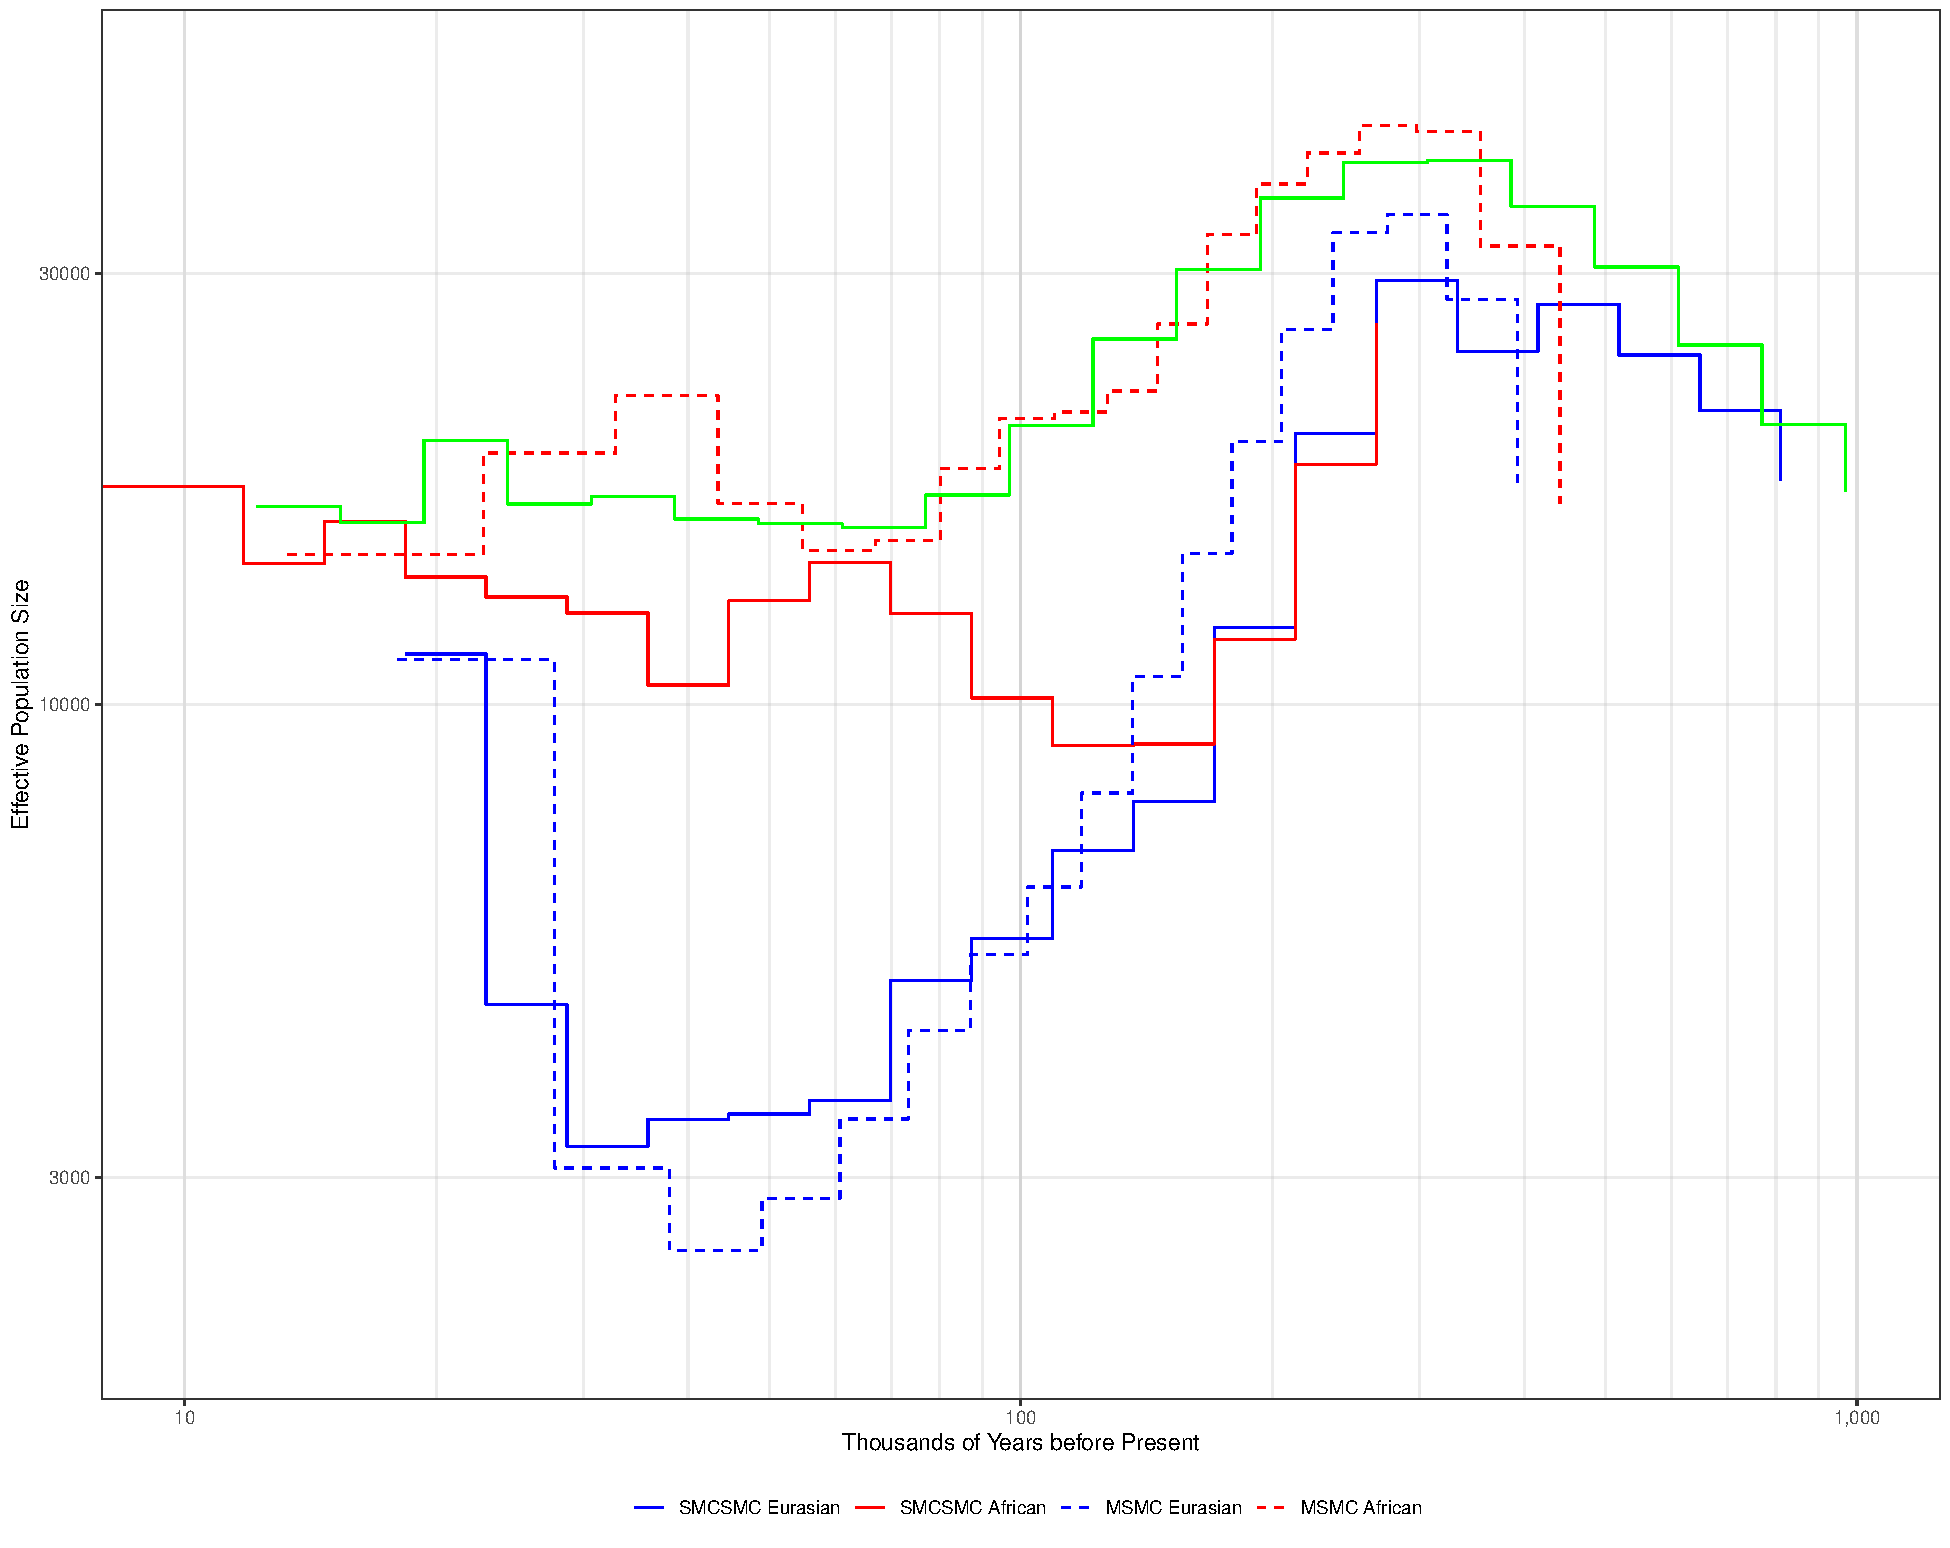
\includegraphics[width=\textwidth]{../plot/ne/figure.pdf}
	\caption{Inferred effective population size using {\tt smcsmc} and MSMC from real and simulated whole genome sequence data. A. Inferred $N_e$ of Han Chinese and Yoruban individuals from the SGDP in both MSMC and {\tt smcsmc}. B. $N_e$ of Han Chinese and Yoruban individuals from the physically phased subset of the HGDP. C, D, and E simulate demographic histories with a 33\%, 42.5\%, and 50\% total replacement 60kya, over the span of 10ky, in {\tt scrm} and reinfer the $N_e$ with {\tt smcsmc}. We replicate a PSMC-like analysis by analysing one diploid Yoruban with {\tt smcsmc} (PSMC$^2$).}
	\label{neplot}
\end{figure}

%In the populations with this trend, {\tt smcsmc} infers directional migration from Eurasian populations to African ones. Specifically, we select a representative from each African population in the Simons Genome Diversity and model migration to a French, Han, and Papuan individual in different analyses. We initialise the inference with a symmetrical migration equal to 1.00 4$N_0$ proportion replaced per generation (henceforth, we assume an $N_0=14312$ {\bf CITE?}), a choice we justify through simulation in Supplemental Simulation \ref{minit}. A comparable magnitude of migration is found in Niger-Kordofanian and Nilo-Saharan populations, while analysis with Afroasiatic populations shows a sustained history of bidirectional migration consistent with the literature. San groups show a lower degree of migration, which is seen to a lesser degree in Mbuti populations. 

\begin{figure}
	\centering
	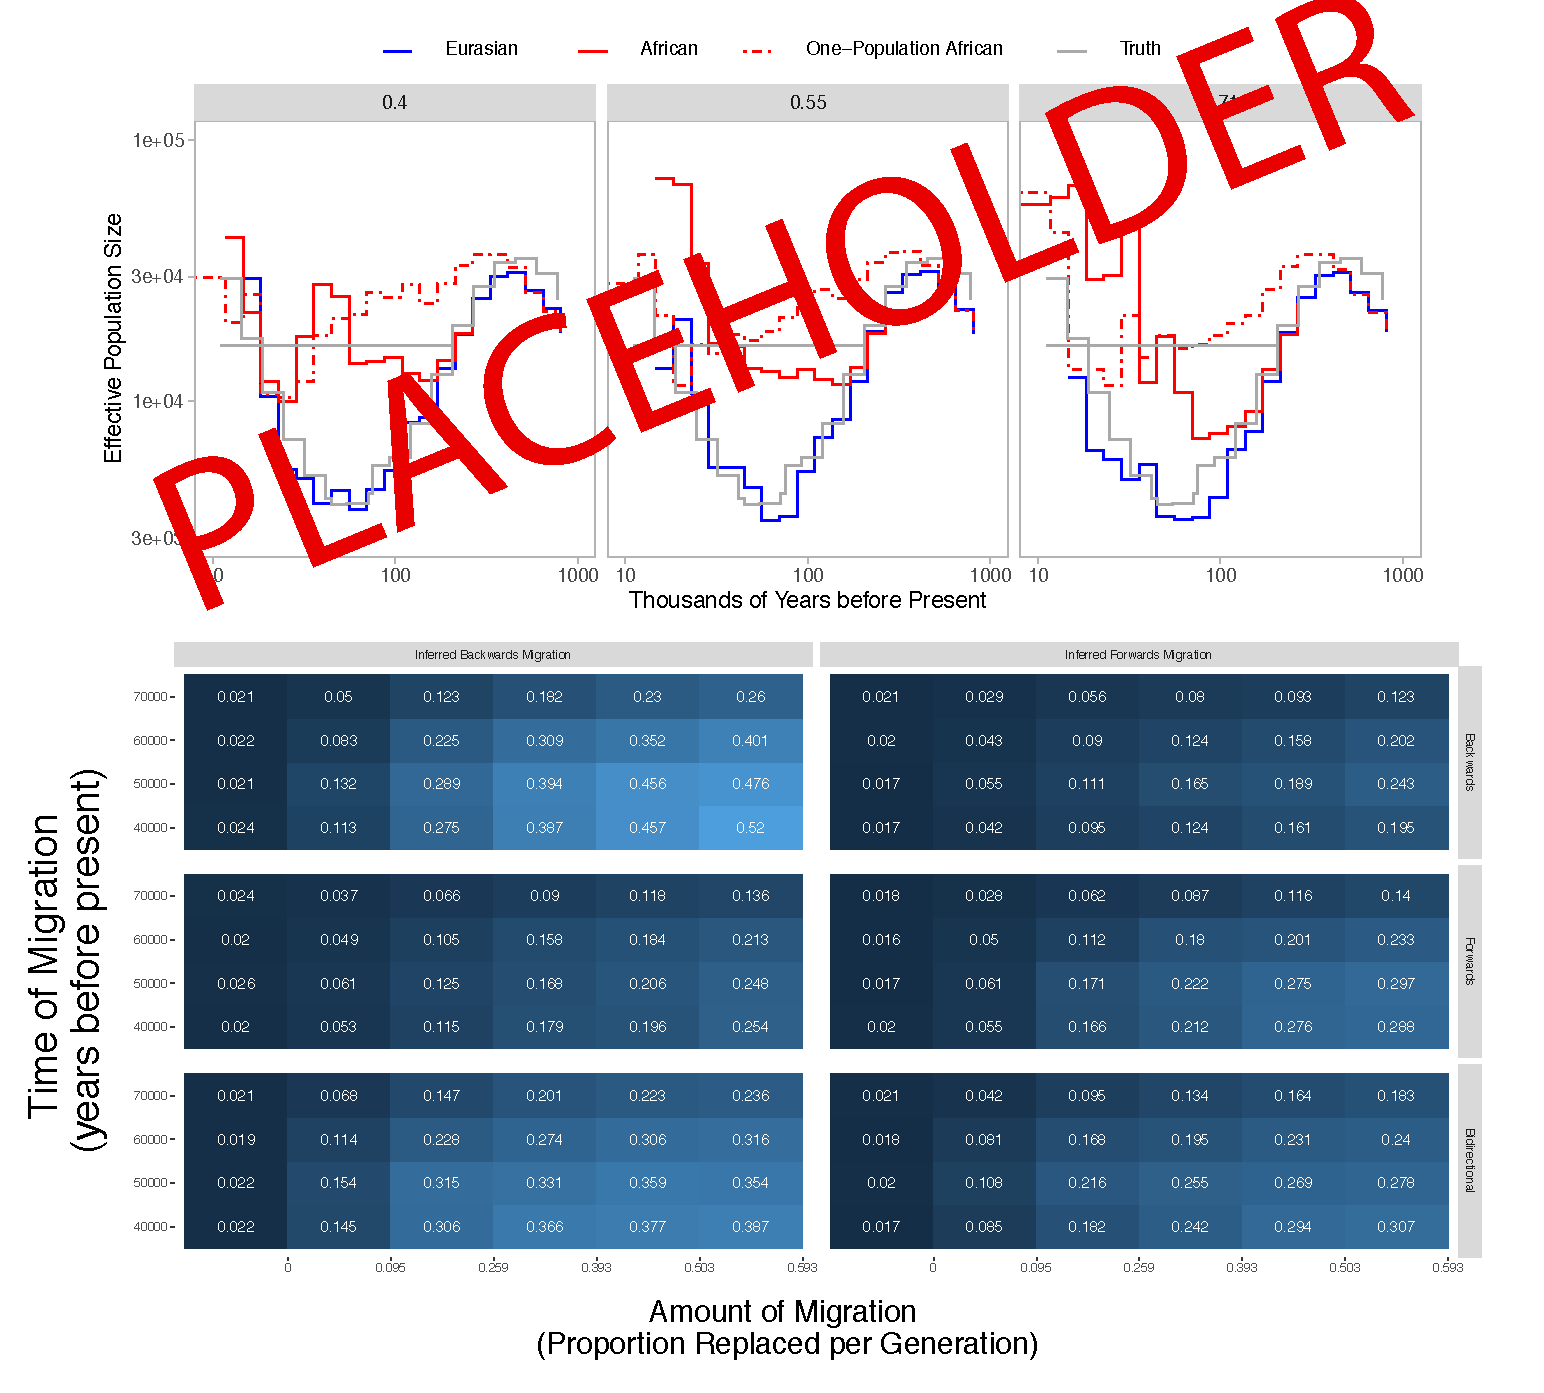
\includegraphics[width=\textwidth]{../plot/ne/PLACEHOLDER_sims.pdf}
	\caption{Simulation study concludes that {\tt smcsmc} has power to detect a back-migration. Top: One gigabase of sequence was simulated by {\tt scrm} under models with increasing migration from an ``African'' population to a ``Eurasian'' population. The magnitude of the population replaced by the migration is indicated in the grey ribbon. In Figure S we additionally vary the timing and duration of the migration, which for this figure are fixed at 60kya and 10ky respectively. Dotted line indicates a single diploid ``African'' genome which was analysed in a one-population model. Grey indicates the true population size simulated. Bottom: Under three different scenarios (migration ``backwards'' from Eurasia to Africa, migration ``forwards'' from Africa to Eurasia, and ``bidirectional'' migration, all forward in time), {\tt scrm} was used to simulate one gigabase of sequence and 5 iterations of {\tt smcsmc} with 5000 particles were used to infer migration. The axis of each heatmap shows increasing simulated proportion replaced over 100,000 while the Y shows the midpoint of the migration simulated. The full migration and population size inference over time along with a more substantial set of simulations is available in Supplemental Section \ref{simproc}.}
	\label{sim}
\end{figure}

\begin{figure}
	\centering
	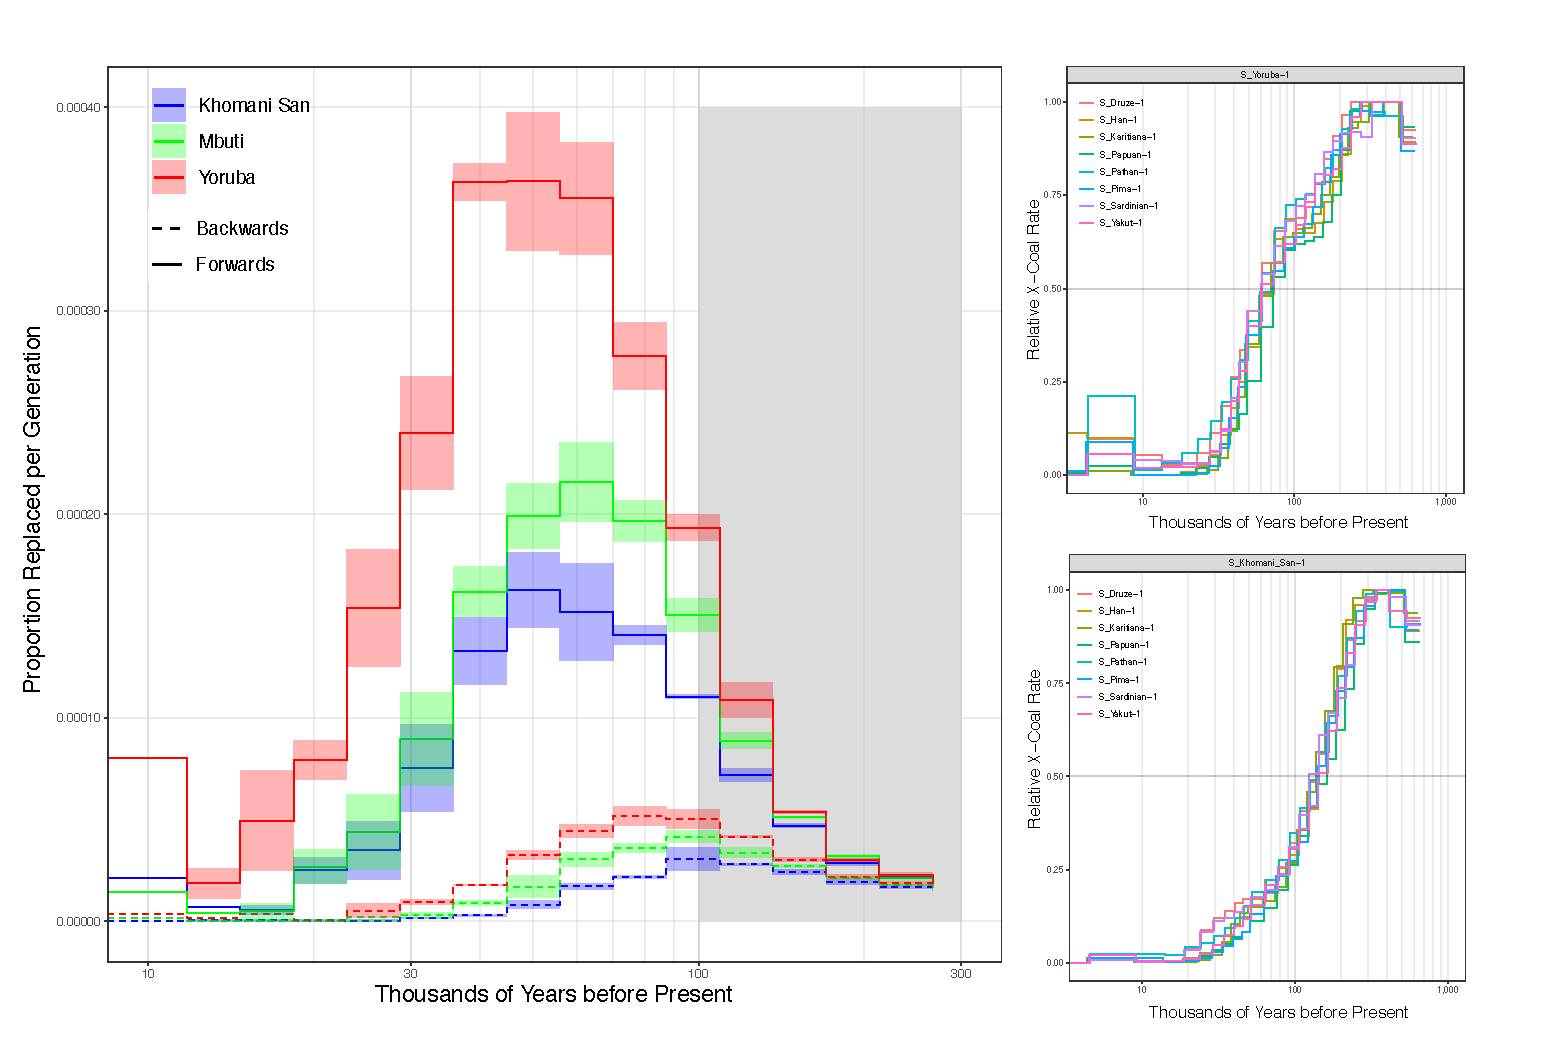
\includegraphics[width=\textwidth]{../plot/mig/mig.pdf}
	\caption{Migration estimates from the Simons Genome Diversity Panel. A. shows three replicates of {\tt smcsmc} inferred migration to with a Han Chinese individual in three contrasting populations representing Niger-Kordofanian and San populations, with the Mbuti a unique intermediate. Analysis used 10000 particles and 25 iterations of variation Bayesian inference to converge. Trend line represents the mean of the replications, while the shaded regions denote the standard deviation. B. and C. show relative cross-coalescent (x-coal) curves for the Yoruban and San individuals modelled with a panel of Out of Africa OoA populations showing contrasting migration histories.}
	\label{migrationplot}
\end{figure}

\begin{figure}
	\centering
	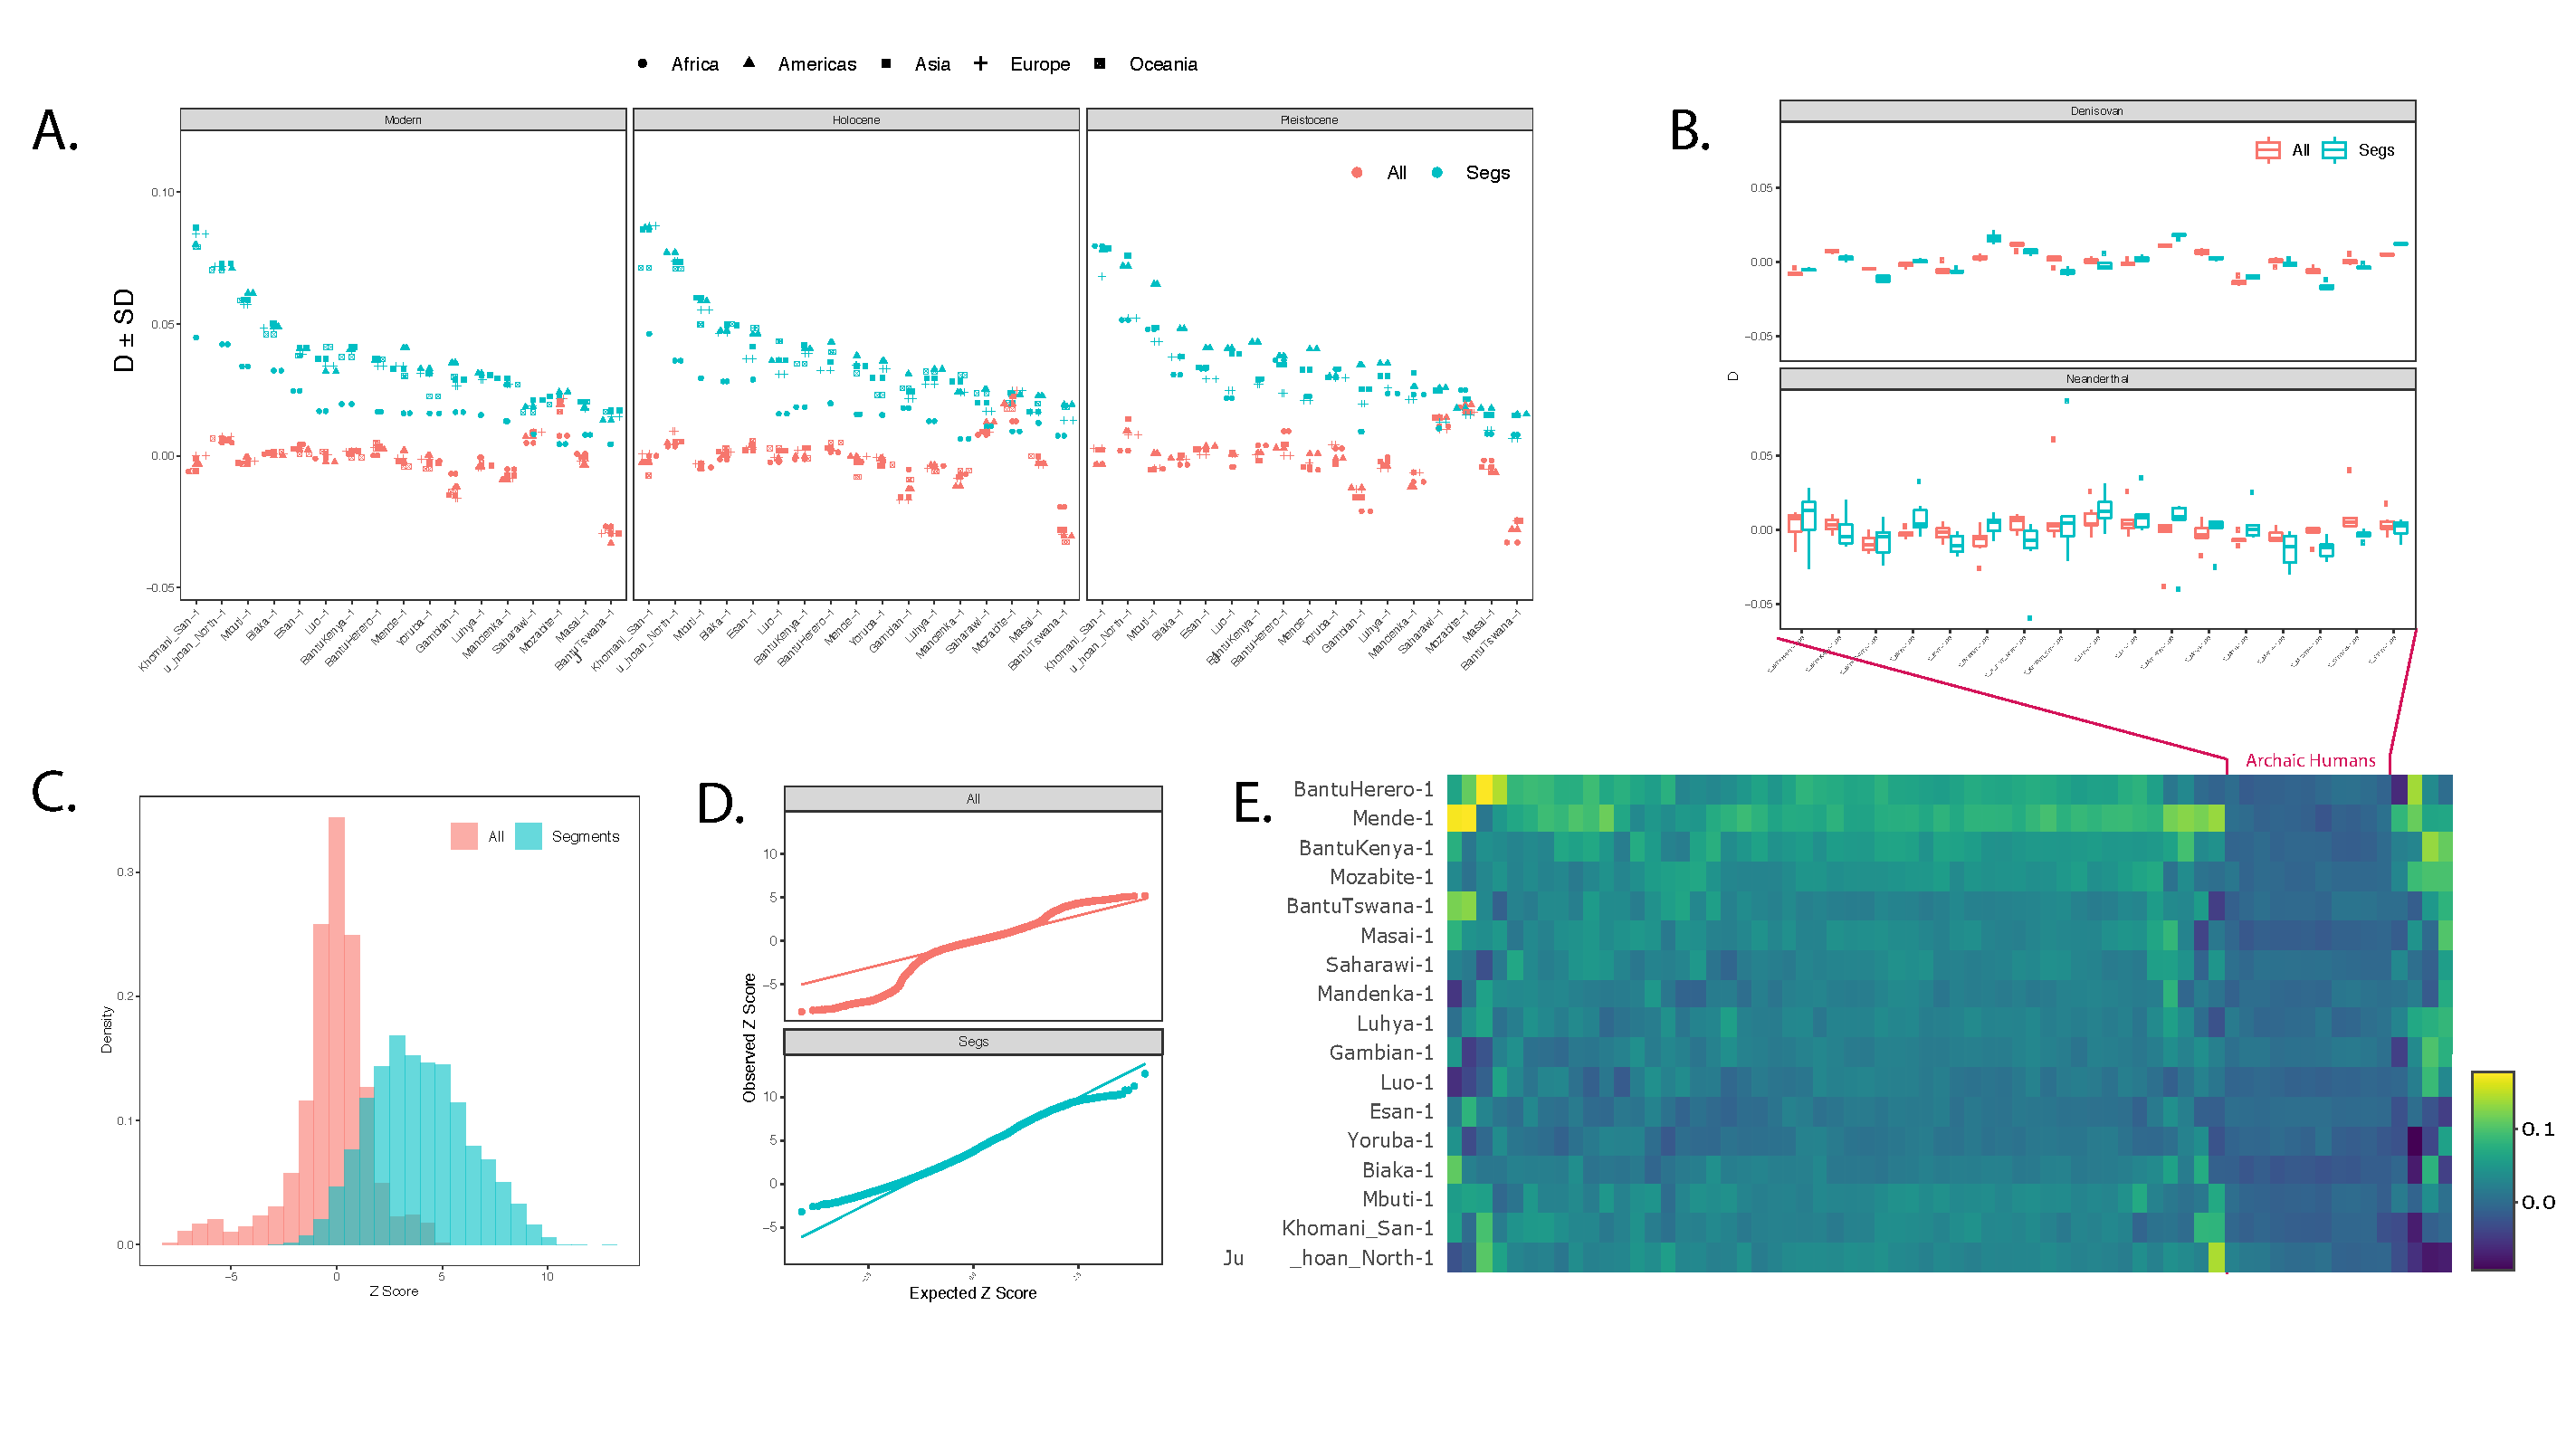
\includegraphics[width=\textwidth]{../plot/dstats.pdf}
	\caption{Analysis of $D(A, A_p, Y, Chimp)$ statistics for all analysed African populations $A$ paired with a partner from the same population $A_p$ and analysed for gene flow with a global population $Y$ from the Reich Lab genotype database. A. compares average $D$ statistic by continent in different African populations, calculated for both all available markers and for the portion of the genome whose tree contains a back-migration event. This is stratified by the age of the comparison sample, either Modern (Present - 1kya), Holocene (1kya - 11.7kya), or Pleistocene ($>11.7$kya). B. displays the distribution of $D$ statistics for both sections, while C. gives a QQ plot of their Z statistics. D. shows a heatmap of D statistics for all of the Pleistocene samples, with E. being a blow-out of the Denisovan and Neanderthal statistics.}
	\label{dstats}
\end{figure}


\begin{figure}
	\centering
	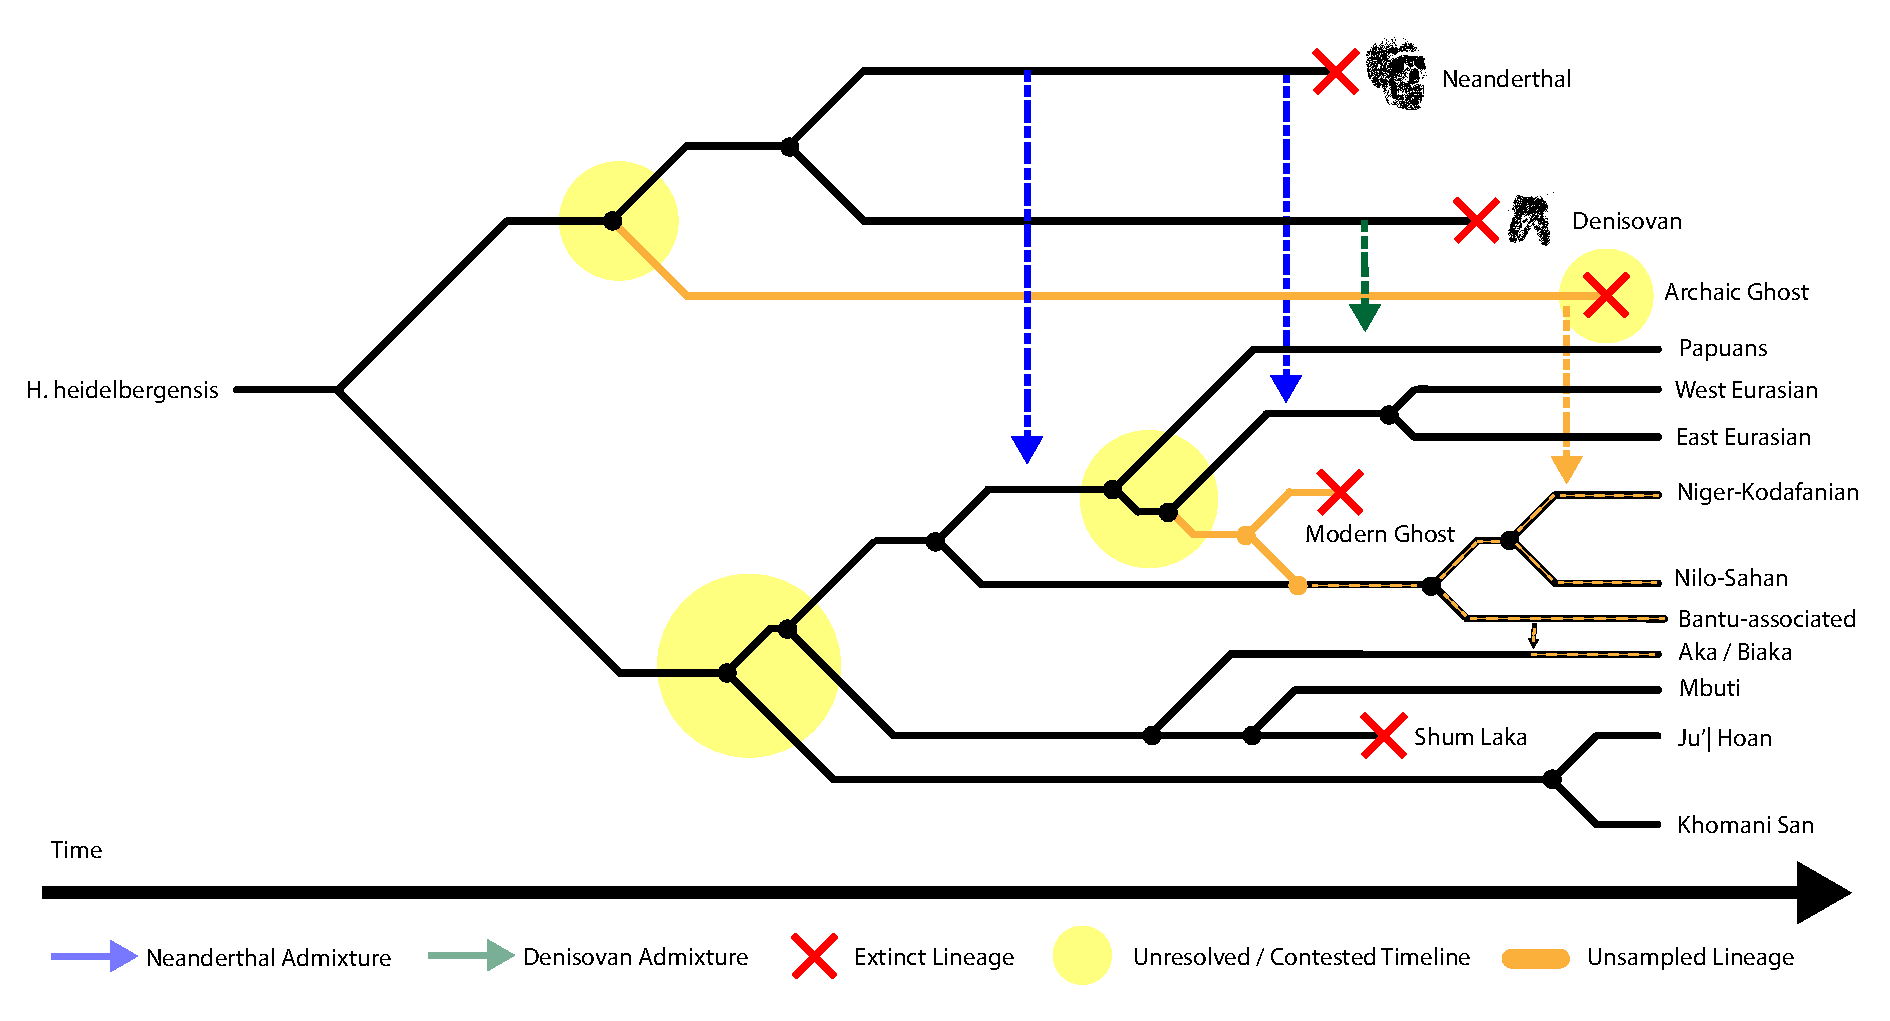
\includegraphics[width=\textwidth]{../plot/dem2.pdf}
	\caption{Proposed Demographic Model. Population splits coloured in yellow are contested. The existance of an archaic ghost lineage which has contributed to Western African populations has been broadly supported in the literature, but the time and order of divergences relative to Neanderthals and Denisovans remains an open question. Until recently, the San peoples were considered to be the most anciently diverged group in Africa, though recent evidence places Central African Hunter Gatherers on a similar timespan, with the addition of a modern ghost population. This existance of this population is additionally supported in the literature and in this article, though the order of divergence is contested. In this article we posit that the ghost diverged from the common ancestor of Eurasians after Papuans had diverged, similar to that suggested in \cite{Malaspinas2016}.}
	\label{fig_dem}
\end{figure}

%\subsection*{URLs}
%\paragraph{Simons Genome Diversity Panel Phased Release} \url{https://sharehost.hms.harvard.edu/genetics/reich_lab/sgdp/phased_data/}
%\paragraph{Human Genome Diversity Panel} \url{ftp://ngs.sanger.ac.uk/production/hgdp/hgdp_wgs.20190516/}
%\paragraph{Ancient DNA} \url{http://cdna.eva.mpg.de/neandertal/}
%\paragraph{Strict 1000 Genomes Accessibility Mask} \url{ftp://ftp.1000genomes.ebi.ac.uk/vol1/ftp/release/20130502/supporting/accessible_genome_masks/}
%\paragraph{SMCSMC Implementation} \url{https://github.com/luntergroup/smcsmc}
%\paragraph{vcf2eigenstrat} \url{https://github.com/bodkan/vcf2eigenstrat}
%\paragraph{ADMIXTOOLS} \url{https://github.com/DReichLab/AdmixTools}
%\paragraph{admixr} \url{https://github.com/bodkan/admixr}

\missingfigure[]{Table for important D statistics like in Prufer 2011}

\newpage
\emergencystretch=1em
\printbibliography

\newpage
\setcounter{section}{0}
\renewcommand{\thesection}{S\arabic{section}}%
\setcounter{table}{0}
\renewcommand{\thetable}{S\arabic{table}}%
\setcounter{figure}{0}
\renewcommand{\thefigure}{S\arabic{figure}}%


\section{Details of Data Analysis}

\subsection{Inferring population size and migration rates in the Simons Genome Diversity Panel}

This section describes analysis of the Simons Genome Diversity Panel with both {\tt smcsmc} and MSMC. {\tt smcsmc} version 1.0.1 was installed from the conda package manager (also found at \url{https://github.com/luntergroup/smcsmc/releases/tag/v1.0.1}), MSMC version 1.1.0 was installed from Github (found at \url{https://github.com/stschiff/msmc/releases/tag/v1.1.0}) and all analyses were performed on the Oxford Biomedical Research Computation cluster.

We download prephased sequencing data from \url{https://sharehost.hms.harvard.edu/genetics/reich_lab/sgdp/phased_data/} and mask for the strict accessibility mask from the 1000 genomes project. We additionally mask for any sites absent Chimpanzee ancestry due to a known issue with the phasing algorithm. We do this masking in {\tt vcftools}. We use {\tt smcsmc} to convert the sequence data from VCF to seg file format, a format very similar to MSMC format. We provide a script to convert from seg file format to MSMC file format as well. Unless otherwise noted, the names of individuals used in this paper are the first in their population (i.e. an individual named Yoruban is {\tt S\_Yoruba-1} in the SGDP nomenclature). We select two diploid individuals from each population in Africa  and infer piecewise constant population size and directional migration rates. Specifically, we use the following options for {\tt smcsmc}:

\begin{verbatim}
smc2 -c -chunks 100 -no_infer_recomb -nsam 4 -I 2 2 2
-mu 1.25e-8 -rho 3e-9 -calibrate_lag 1.0 -EM {EM} 
-tmax 3.5 -alpha 0.0 -apf 2 -N0 14312 -Np {Np} -VB 
${DEMOGRAPHIC_MODEL} -P 133 133016 31*1 
-arg -o ${OUTPUT} -segs ${SEGS}
\end{verbatim}

In order, we invoke the use of a QSUB cluster with {\tt -c} and split our analysis into 100 chunk. We do not infer recombination sites along with the demographic model in order to reduce runtime. Four haploid samples, two from each population, are analysed with a mutation rate of 1.25 $\times 10^{-8}$, a recombination rate of 3 $\times 10^{-9}$, and accumulating events for one unit of survival time along the sequence. We use a given number of epochs for parameter units, and bound the upper limits of the trees at 3.5 times the effective population size (set to 14312). We use the lookahead likelihood to guide the resampling process for a given number of particles {\tt Np} and use variational Bayes in place of the default stochastic expectation maximization algorithm. Parameters are inferred over 31 equally spaced intervals from 133 to 133016 generations in the past, and the sampled posterior ARGs are reported. 

We seed the particle filter with a demographic model of population size and uniform symmetric migration rate, given by the following {\tt scrm} command:

\begin{verbatim}
-ej 0.2324 2 1 -eM 0 1 -eN 0.0 6 -eN 0.0037 4.4 -eN 0.0046 3 
-eN 0.0058 2 -eN 0.0073 1.4 -eN 0.0092 0.85 -eN 0.093 1.2 
-eN 0.12 1.7 -eN 0.15 2.2 -eN 0.19 2.5 -eN 0.24 2.4 -eN 0.30 2.0 
-eN 0.37 1.7 -eN 0.47 1.4 -eN 0.59 1.2 -eN 0.74 1.0 
-eN 0.93 0.91 -eN 1.2 1.6
\end{verbatim}

We visualise this demographic model in the POPdemog package in Figure \ref{smc2demog}.

\begin{figure}
	\centering
	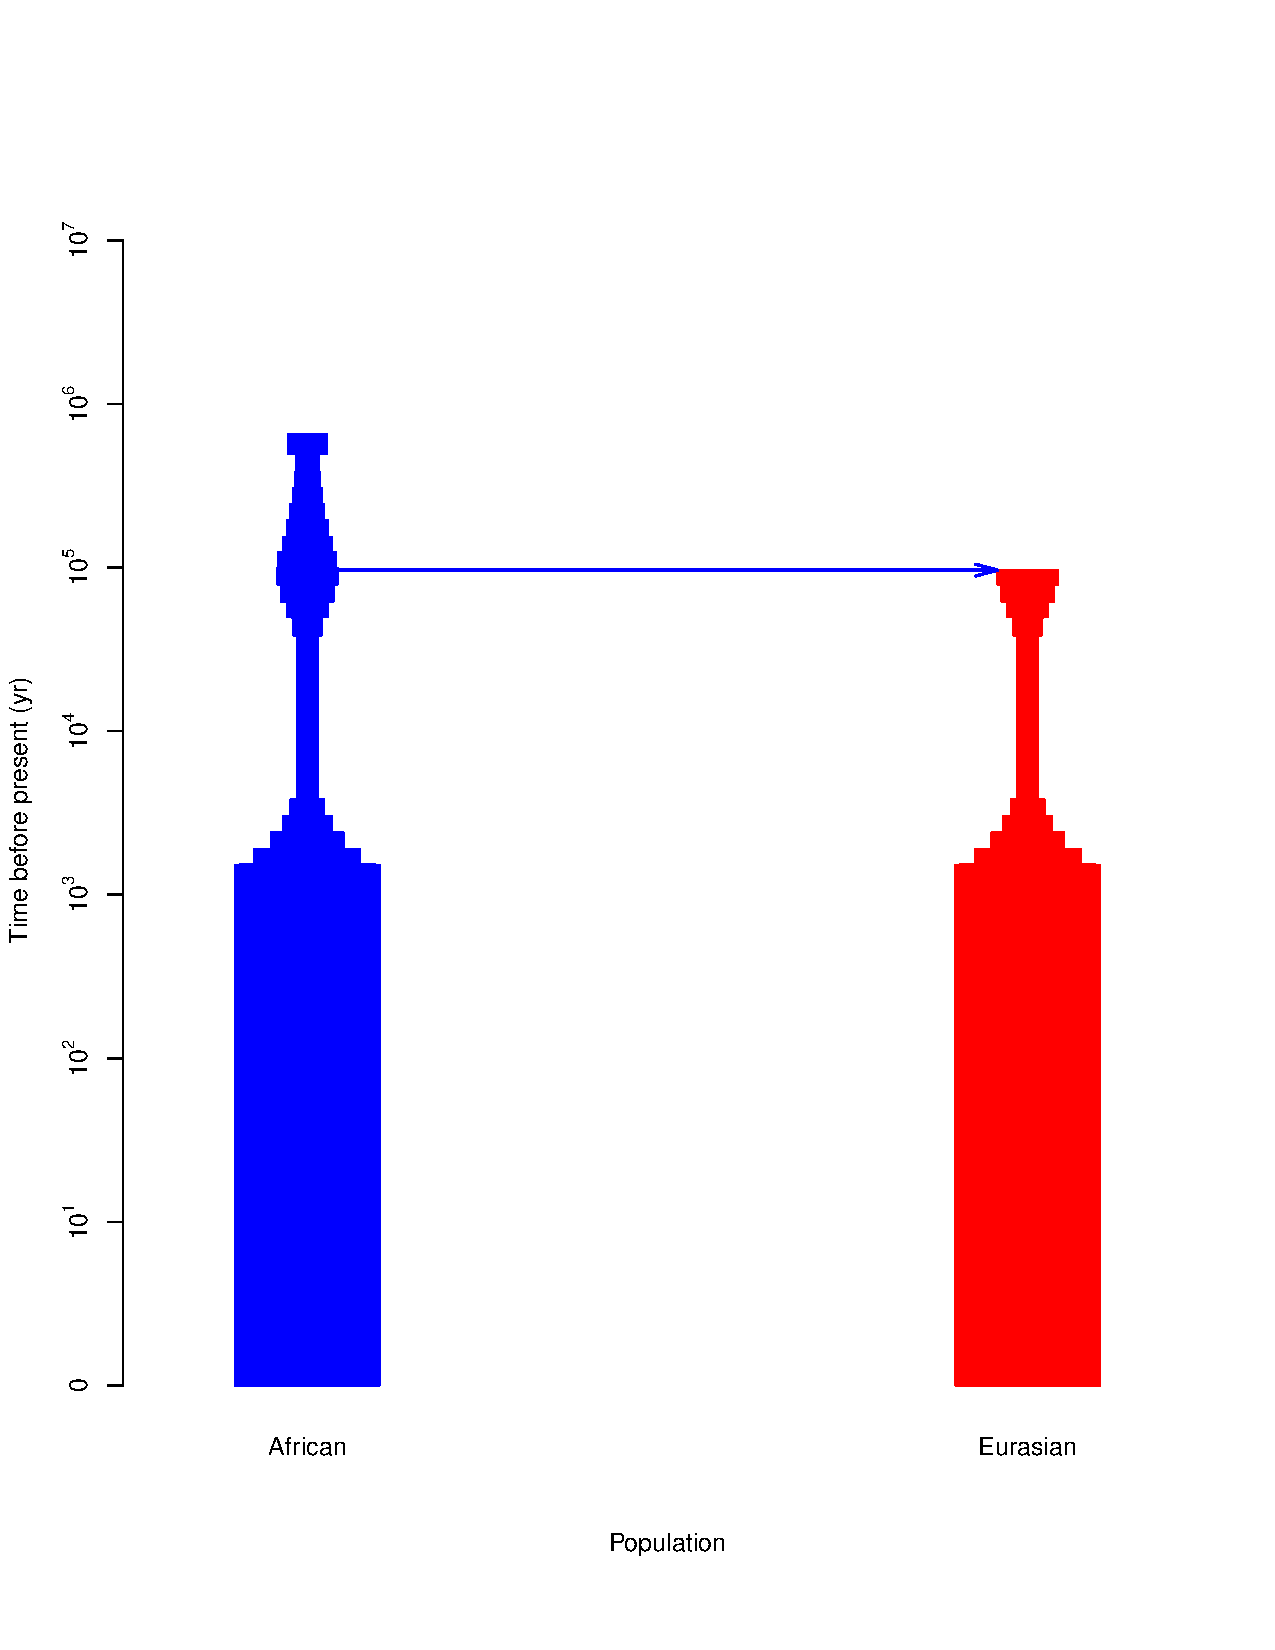
\includegraphics[width=0.25\textwidth]{../plot/dem_smc2.pdf}
	\caption{Demographic model used as a seed for SMC2 analysis}
	\label{smc2demog}
\end{figure}

Each {\tt smcsmc} analysis gives a final output file detailing migration and coalescent events, their rates, and their opportunities which denote the total opportunity for an event to occur during a particular epoch. Output files are trimmed to only visualise the final epoch of variational Bayes inference and assessed for convergence. Times and rates are interpreted differently than {\tt scrm} output. Rates are in units of $4N_0$ per generation, while times are given in generations. 

We implement the above in an open source {\tt Snakemake} pipeline at \url{SNAKEM} which also implements a default analysis of MSMC with forty iterations to converge. Sample size and relative cross-coalescent rates are transformed as described in the documentation using the same parameter values for mutation rate and generation time used for {\tt smcsmc} analysis. Effective population size and migration estimates for the populations analysed in the SGDP are given in Figures \ref{sgdp_ne} and \ref{sgdp_mig}. MSMC appears to consistently find a higher African $N_e$ in the ancient past until the average estimates across populations stabalises approximately 100kya (Figure \ref{averages}). We expand on a possible rational behind this effect in the main text of this article.

\begin{figure}
	\centering
	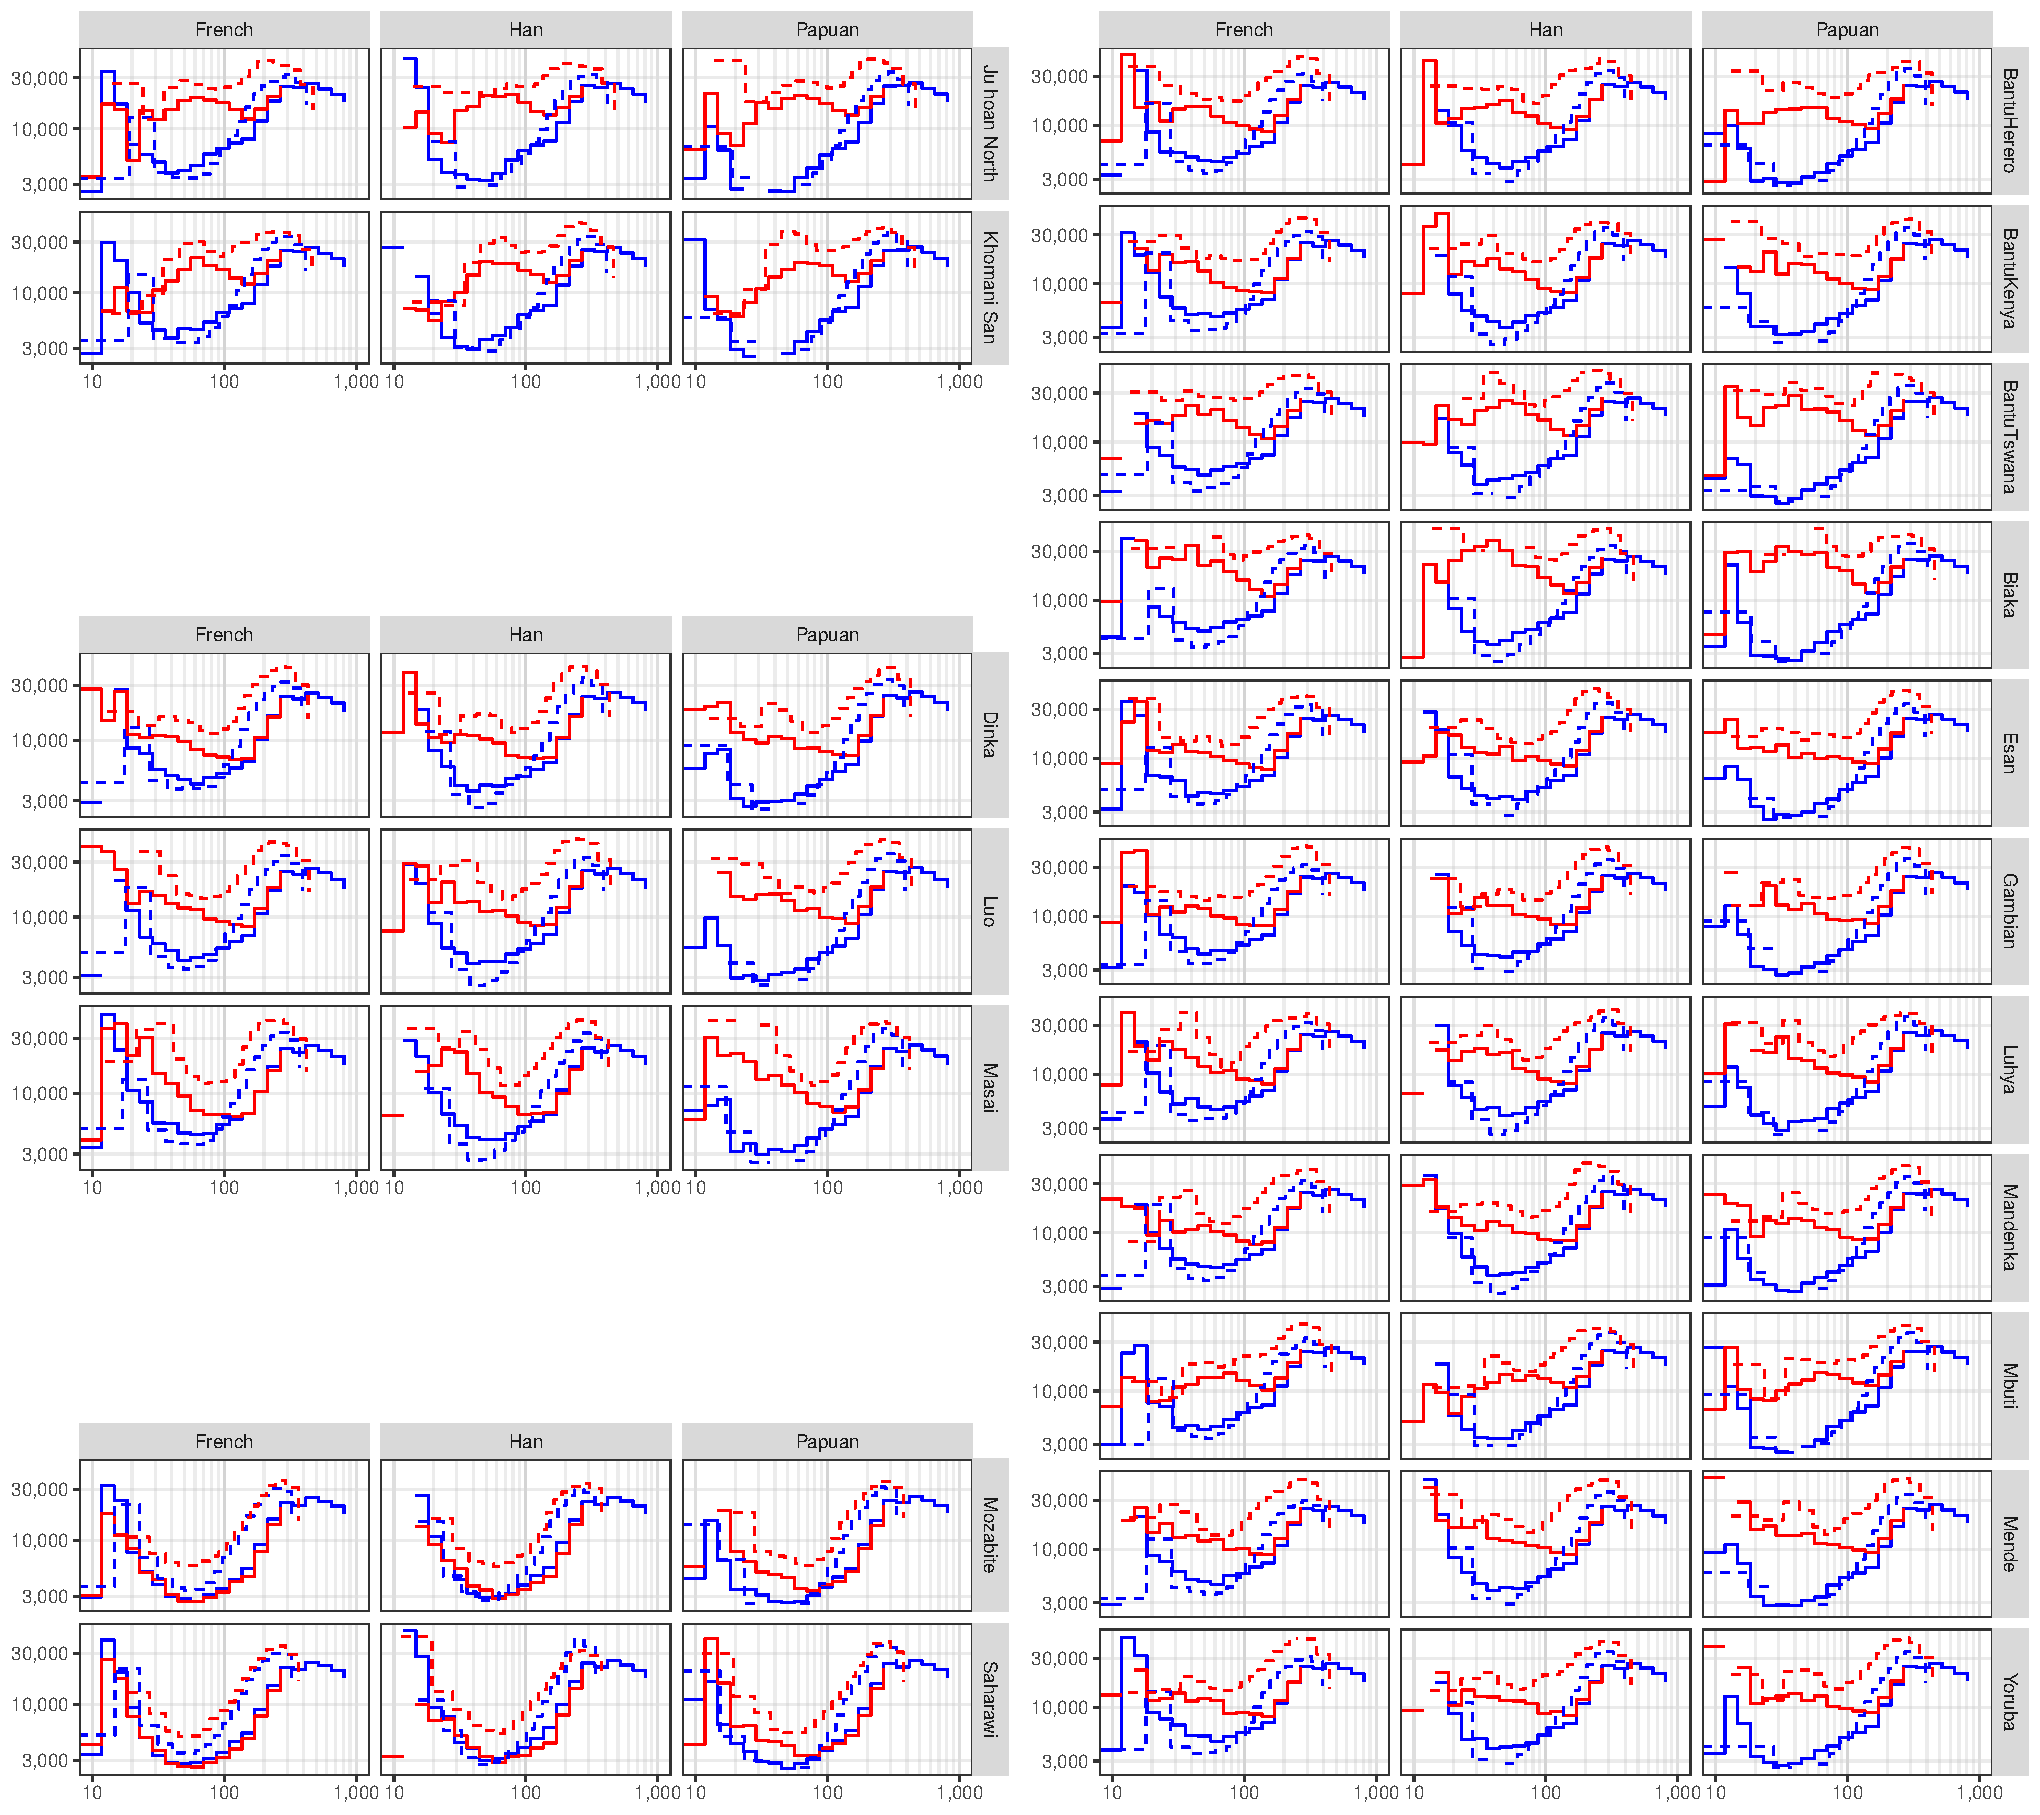
\includegraphics[width=0.75\linewidth]{../plot/sgdp_ne.pdf}
	\caption{Estimated effective population size in different African and Eurasian groups with {\tt smcsmc}. Left: From top to bottom, inferred $N_e$ in Khoesan, Nilo-Saharan, and Afroasiatic populations. Right: Inferred $N_e$ in Niger-Kordofanian populations. 5000 particles and 10 variational Bayes interations were used to achieve convergence.}	
	\label{sgdp_ne}
\end{figure}

\begin{figure}
	\centering
	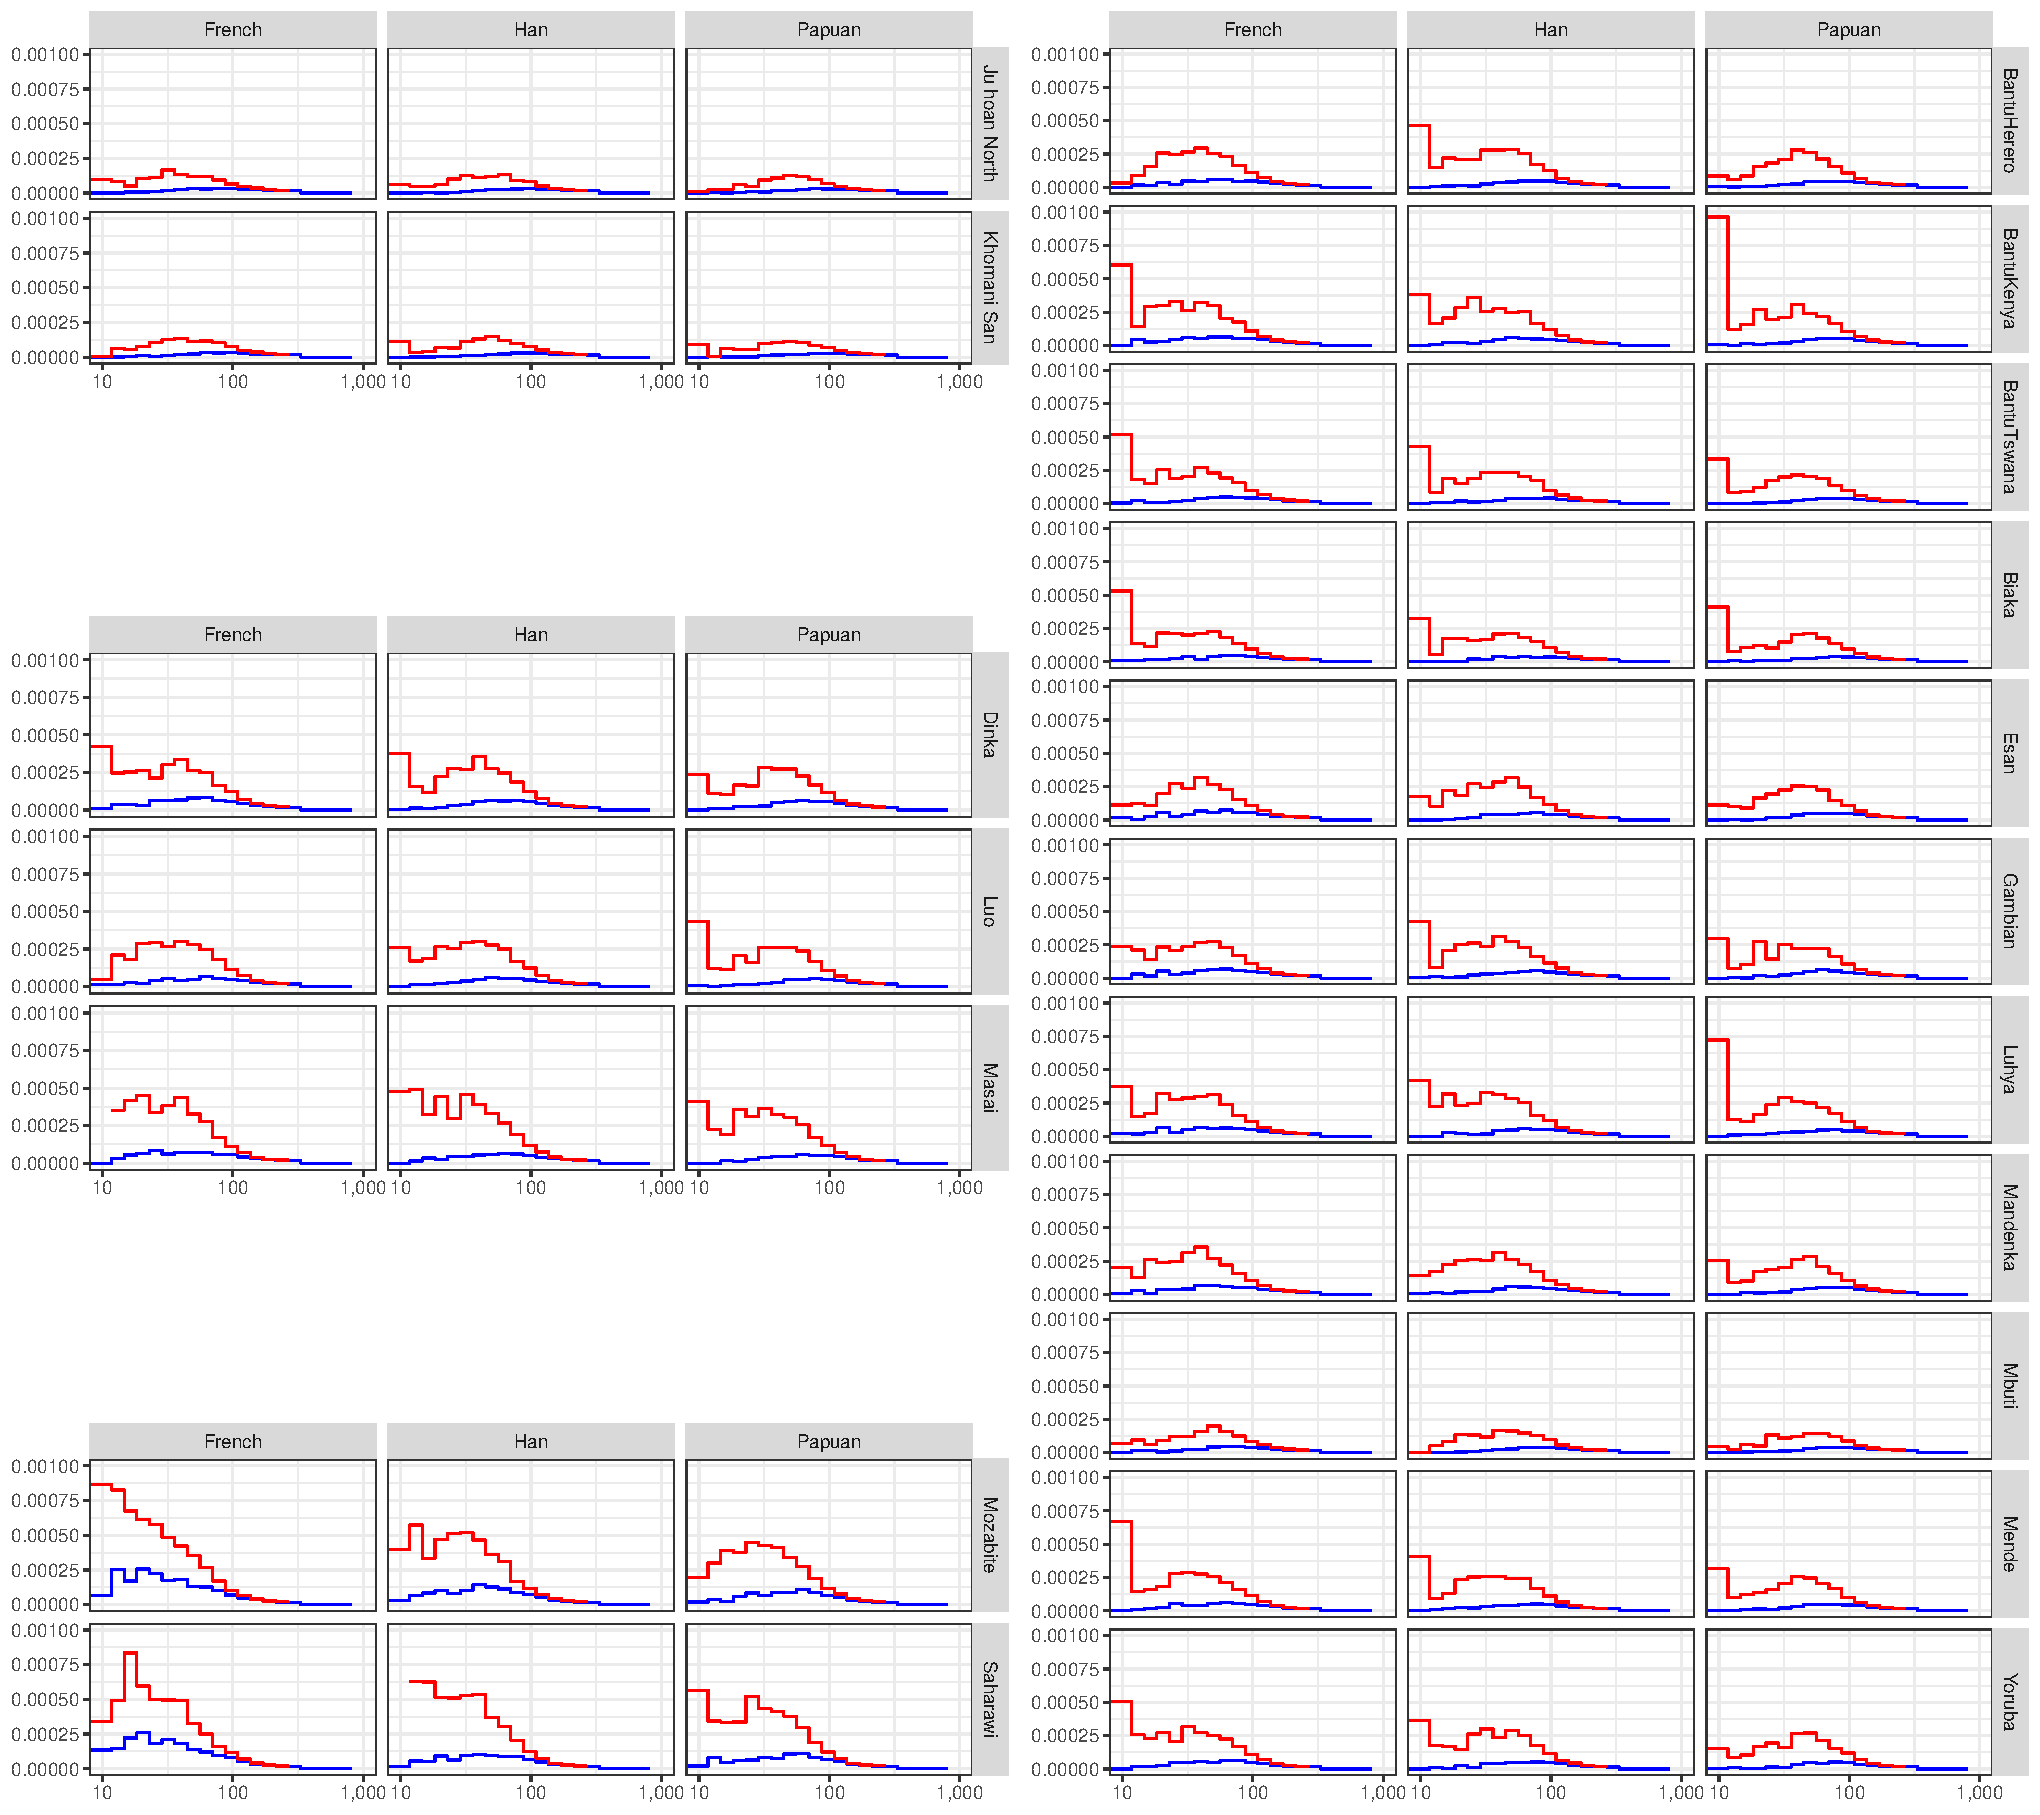
\includegraphics[width=0.75\linewidth]{../plot/sgdp_mig.pdf}
	\caption{Estimated directional migration between African and Eurasian groups in the SGDP with {\tt smcsmc}. Left: From top to bottom, inferred migration in Khoesan, Nilo-Saharan, and Afroasiatic populations. Right: Inferred migration in Niger-Kordofanian populations. 5000 particles and 10 variational Bayes interations were used to achieve convergence.}	
	\label{sgdp_mig}
\end{figure}

\begin{figure}
	\centering
	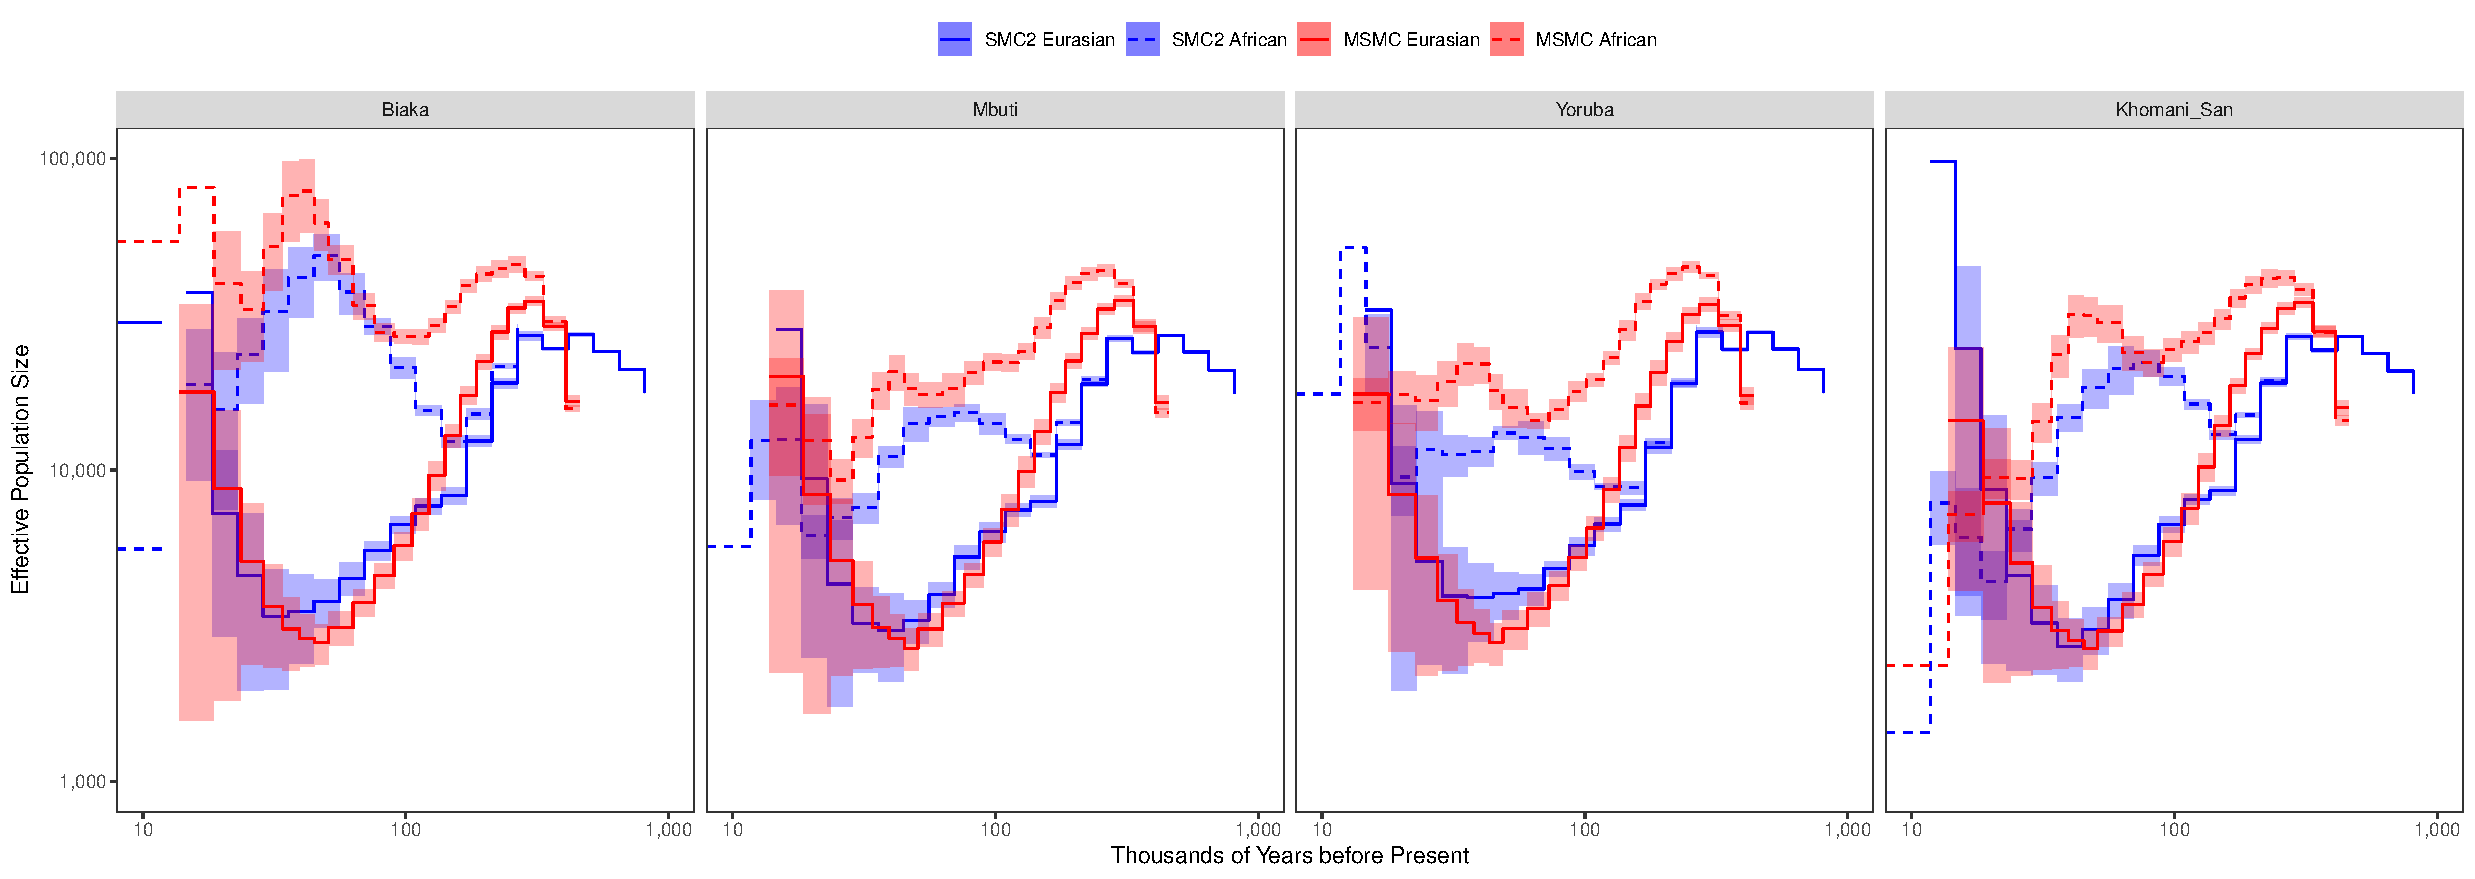
\includegraphics[width=\textwidth]{../plot/ne/average_ne_subset.pdf}
	\caption{Average $N_e$ estimate across four populations in the subset of SGDP used to compare with HGDP inference. Inference of population size is averaged over eight Eurasian populations, with the bars representing standard deviation. For MSMC, the time indexes were averaged to have consistent start and stop times for the steps.}
	\label{averages}
\end{figure}

Migration during the last 100ky is integrated to observe overall trends (Figure \ref{sgdp_heatmap}). We use two methods to integrate migration, the first presented in the main text given by $F(t) = e^{- \int_{t=0}^T \rho(t) dt}$. Alternatively, consider $p$ proportion of the population are replaced every generation. Start with 0 individuals from the source $N_{source}$ population in the sink population $N_{sink}$, each generation replace $p$ proportion of the sink population with the source. We track the proportion of the population which are replaced by the source $P$.  

$$ \begin{aligned} P_0 &= 0 \\ P_1 &= pN_{sink} \\ P_2 &= pN_{sink} + p(N_{sink} - pN_{sink}) \\ &= pN_{sink} + pN_{sink}(1-p) \\ P_3 &= pN_{sink} + pN_{sink}(1-p) + p((N_{sink}-pN_{sink}) - p(N_{sink}-pN_{sink})) \\ &= pN_{sink} + pN_{sink}(1-p)+p(N_{sink}(1-p)-pN_{sink}(1-p)) \\ &= pN_{sink}+pN_{sink}(1-p)+pN_{sink}(1-p)(1-p) \\ &\dots \\ P_n &=N_{sink}p(1-p)^n \end{aligned} $$

In practice, both methods give essentially identical proportions for all considered questions. Inferred migration varies across language groups (Figure \ref{averages_of_sgdp}. Afroasiatic groups show high migration from Han and French populations, with a lower proportion deriving from Papuans. Niger-Kordofanian and Nilo-Saharan groups show an intermediate magnitude, between 50 and 60 percent replacement, though also significantly (P < 0.05, two-tailed paired $T$ test) closer to French and Han sources than Papuans. The Khoesan show the lowest migration, consistent with their early diversification from the remainder of African groups and the relative lack of gene-flow from Western African populations \cite{Lipson2019}. This is contrasted with the Mbuti and Biaka, Central African Hunter Gatherer populations who have historically recieved substantial amounts of gene flow from Western African sources. Both of these populations show the lowest migration in their language group (Table \ref{average_sgdp_migration_table}). 

\begin{figure}
	\centering
	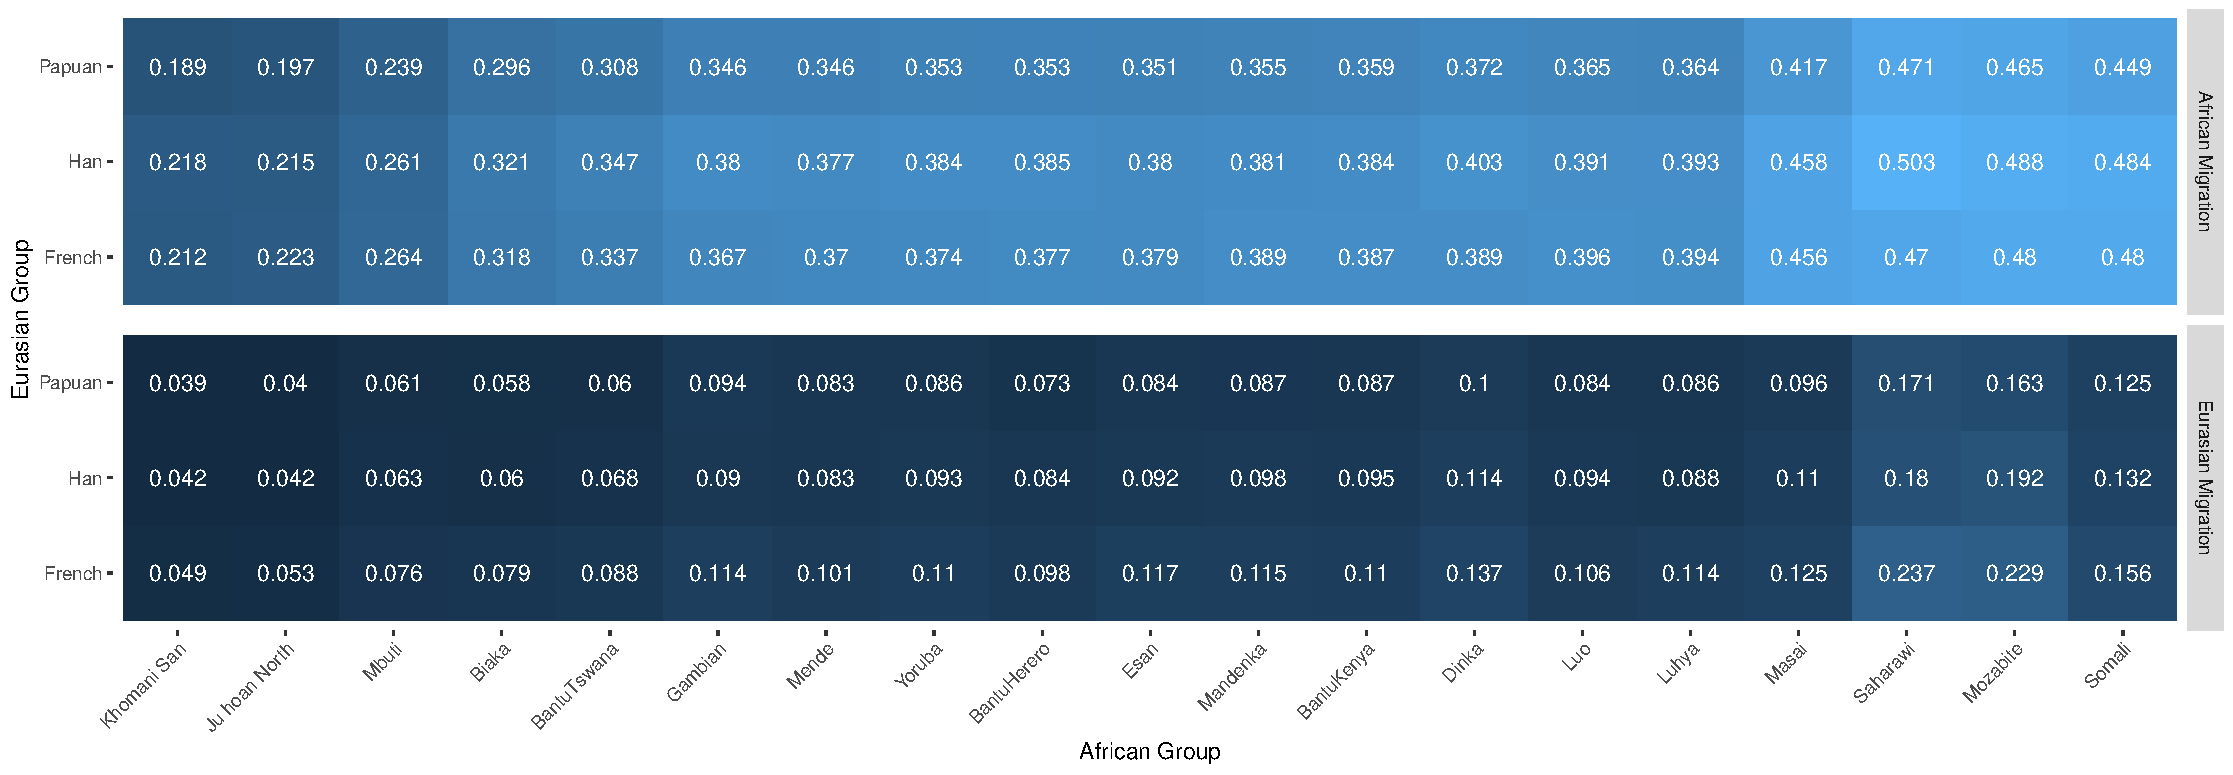
\includegraphics[width=\textwidth]{../plot/mig/integrated_sgdp.pdf}
	\caption{Integrated migration proportion in {\tt smcsmc} analysed SGDP populations.}
	\label{sgdp_heatmap}
\end{figure}

\begin{figure}
	\centering
	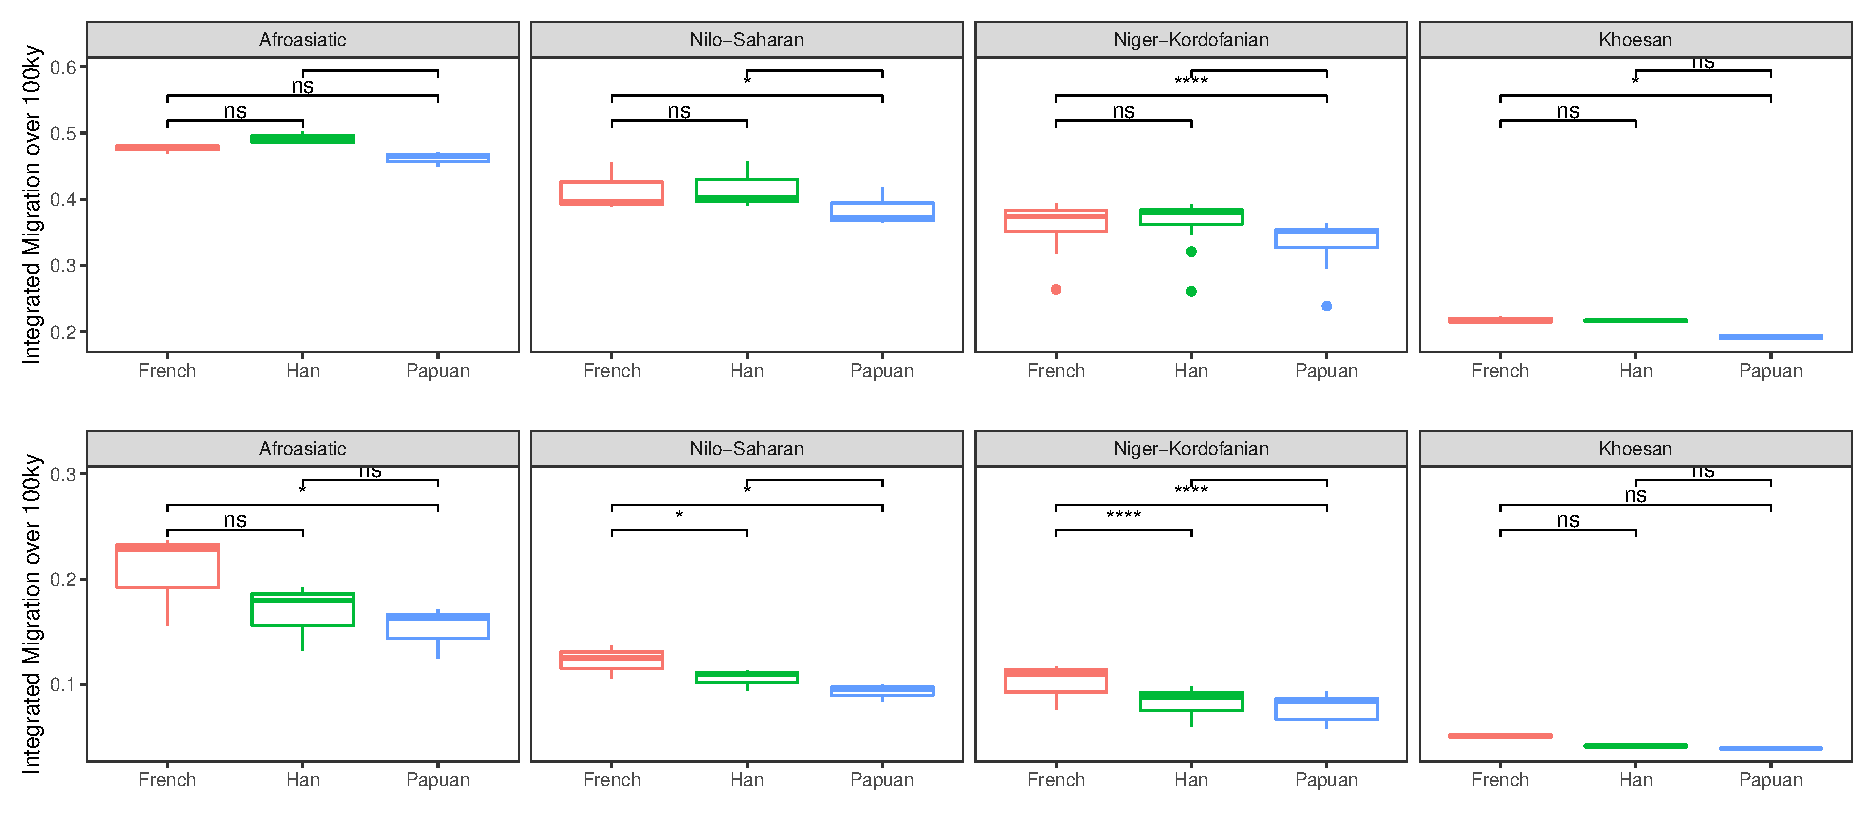
\includegraphics[width=\textwidth]{../plot/mig/sgdp_averages.pdf}
	\caption{Integrated migration proportion over the last 100 thousand years (ky) between language families by comparison population. Papuans contributed significantly less to African populations across all populations in a two tailed paired T test. ns = Not Significant, * = $P<0.05$, ** = $P<0.01$, *** = $P<0.001$, **** = $P<0.0001$.}
	\label{averages_of_sgdp}
\end{figure}

% latex table generated in R 3.5.3 by xtable 1.8-3 package
% Wed Jan 22 11:49:06 2020
\begin{table}[ht]
	\centering
	\begin{tabular}{llll}
		\hline
		African & Eurasian & $M_{E, A}$ (SD) & $M_{A, E}$ (SD) \\ 
		\hline
		Afroasiatic & French & 0.722(0.014) & 0.351(0.092) \\ 
		Afroasiatic & Han & 0.721(0.029) & 0.241(0.055) \\ 
		Afroasiatic & Papuan & 0.642(0.018) & 0.218(0.043) \\ 
		Khoesan & French & 0.304(0.005) & 0.079(0.006) \\ 
		Khoesan & Han & 0.292(0.002) & 0.065(0.004) \\ 
		Khoesan & Papuan & 0.257(0.001) & 0.063(0.004) \\ 
		Niger-Kordofanian & French & 0.514(0.059) & 0.151(0.024) \\ 
		Niger-Kordofanian & Han & 0.513(0.061) & 0.121(0.016) \\ 
		Niger-Kordofanian & Papuan & 0.462(0.059) & 0.114(0.016) \\ 
		Nilo-Saharan & French & 0.595(0.079) & 0.186(0.028) \\ 
		Nilo-Saharan & Han & 0.581(0.055) & 0.152(0.012) \\ 
		Nilo-Saharan & Papuan & 0.525(0.048) & 0.134(0.014) \\ 
		\hline
	\end{tabular}
	\caption{Average plus or minus standard deviation integrated directional migration from Eurasian to African populations in the last 100 thousand years (ky)} 
	\label{average_sgdp_migration_table}
\end{table}

\subsection{Validation in a physically phased subset of the Human Genome Diversity Panel (HGDP)} \label{hgdp_section}

For the {\tt smcsmc} algorithm, the use of phased data is not necessary but does help convergence. It additionally helps the lookahead-likelihood to better guide the resampling procedure. Therefore, we do not expect errors made during statistical phasing to significantly impact the inferred parameters. However, to test this, we replicate the above analysis in a physically phased subset of the HGDP downlaoded from \url{ftp://ngs.sanger.ac.uk/production/hgdp/hgdp_wgs.20190516/}. The same {\tt snakemake} pipeline is used as in the analysis of the SGDP data. Data is additionally masked for the filters provided. We plot the effective population size and migration rates in Figures BLAH and BLAH.

{\color{red} All of these (with the exception of one) are complete, but do not have MSMC runs, so there's no use in making all the figures twice.}


\subsection{Patterns in population size and migration fully replicate in an equivalent subset of the SGDP}
To directly compare these results to those obtained in the SGDP, we select the closest matching samples to those in the physically phased HGDP dataset and analyse these with MSMC and {\tt smcmsc} using 10k particles and 25 iterations to achieve convergence (Figure \ref{hgdp_sgdp_ne}). The effective sample size around the OoA migration is similarly inflated in MSMC analyses, while the estimation of the Eurasian population size remains largely consistent.  

\begin{figure}
    \centering
    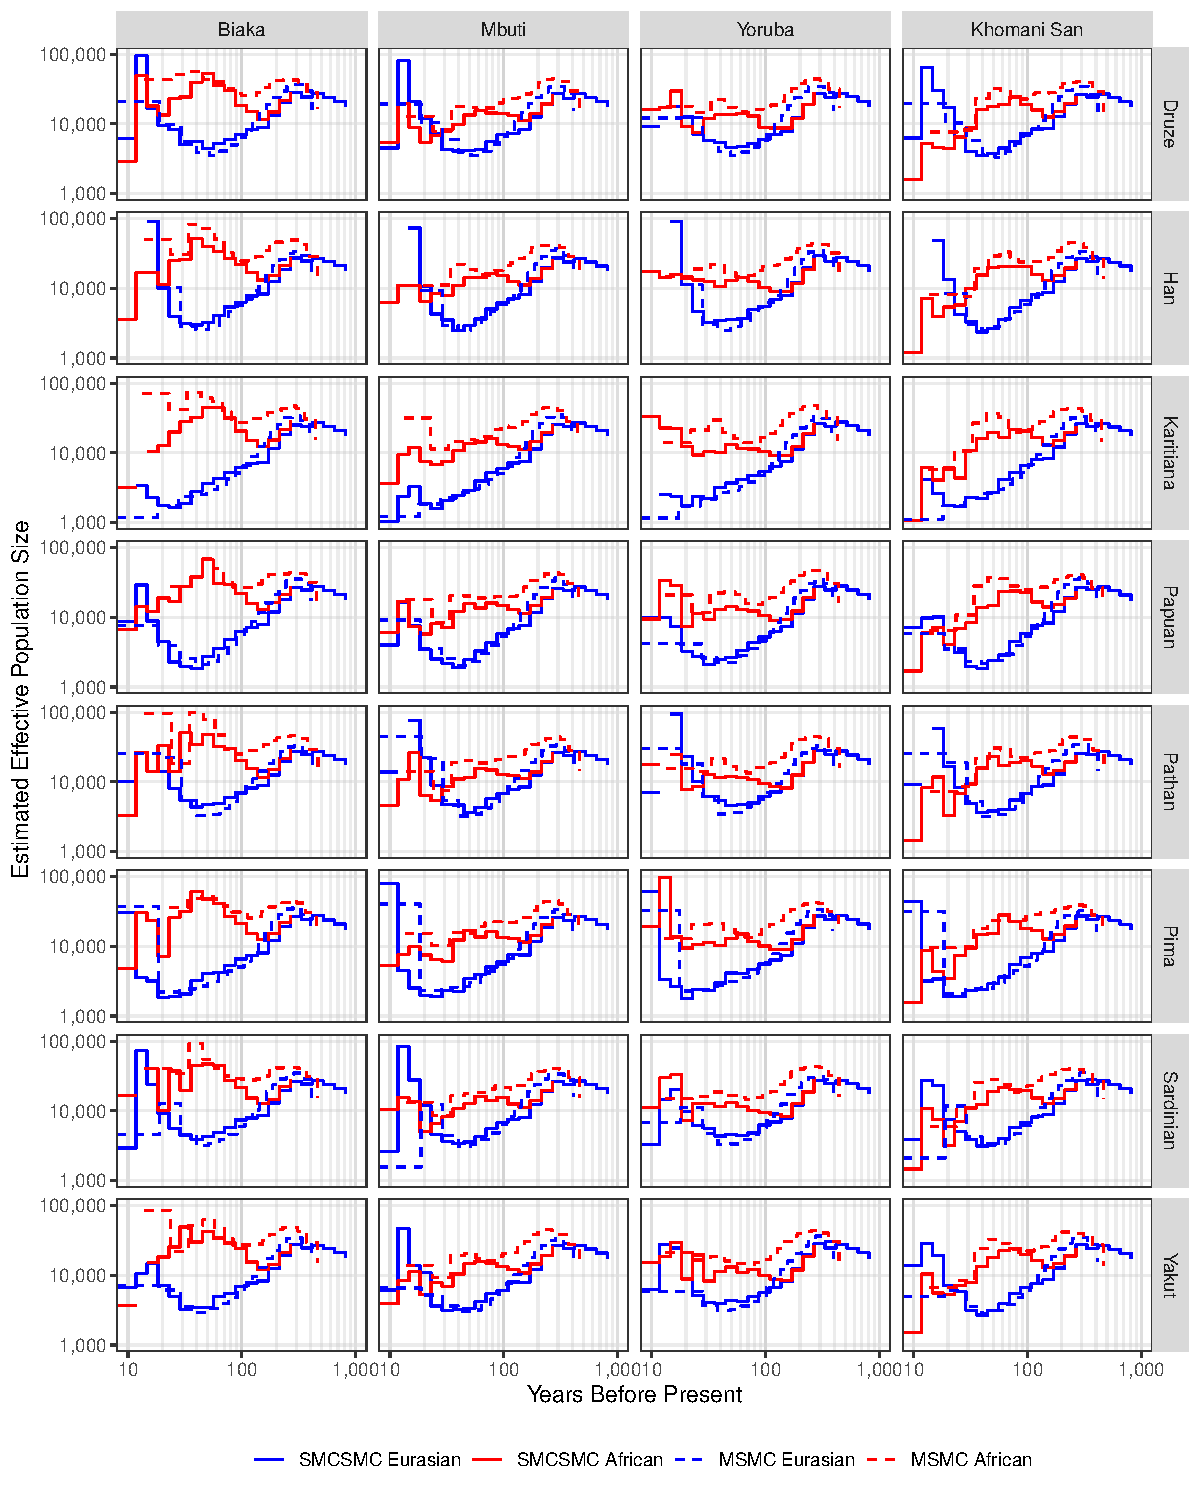
\includegraphics[width=0.9\textwidth]{../plot/sgdp_subet_ne.pdf}
    \caption{{\tt smcsmc} and MSMC inferred effective population size of several populations in the Simons Genome Diversity Panel. These samples were selected to match, as closely as possible, those in the physically phased subet of the Human Genome Diversity Project panel. 10,000 particles and 25 iterations were used for {\tt smcsmc} and 40 iterations for MSMC.}
    \label{hgdp_sgdp_ne}
\end{figure}

\begin{figure}
	\centering
	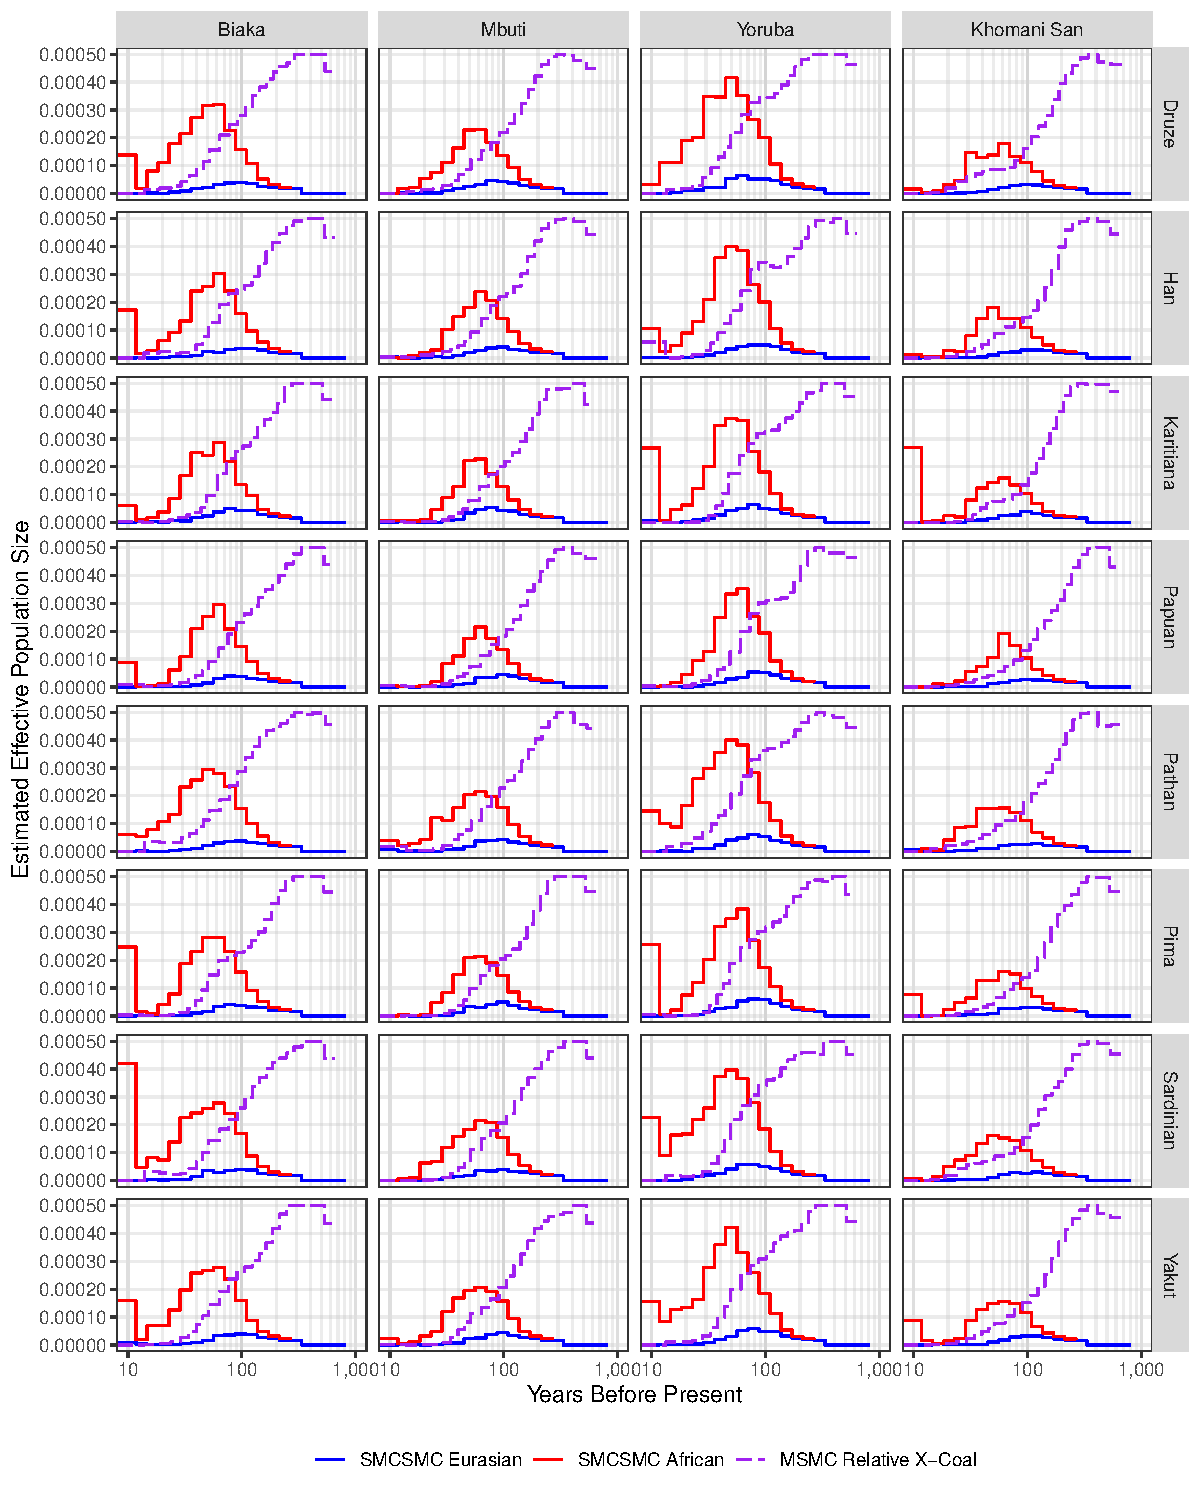
\includegraphics[width=0.9\textwidth]{../plot/sgdp_subet_mig.pdf}
	\caption{Inferred migration using {\tt smcsmc} in the Simons Genome Diversity Panel along with the scaled relative cross-coalescent rate estimated by MSMC. Samples were chosen to match, as closely as possible, those in the physically phased subset of the Human Genome Diversity Project panel. 10,000 particles and 25 iterations were used, 40 in the case for MSMC.}
	\label{fig:hgdp_sgdp_mig}
\end{figure}

\clearpage
\section{Statistical Analysis of Migrated Segments} \label{dstats_section}

We run {\tt smcsmc} with the {\tt -arg} flag to report the posterior estimate of the ancestral recombination graph. We use this to isolate segments of the African genome where predicted migration events occurred between 50 and 70kya and used these segments to calculate drift statistics. Here, Yoruba-1 is used as a representative of Western African groups, and used for ascertaining putatively migrated segments. The two Yorubans share more alleles than other groups in Africa (D(African group, Yoruba-1; Yoruba-2, Chimp) is significantly negative with $|Z|>3$), but the individual of interest is closer to Out of Africa (OoA) groups such as the Han, French, and Papauns (D(OoA, Yoruba-2; Yoruba-1, Chimp) is significantly negative with $|Z|<3$) than to its partner Yoruban (Table \ref{dstats:a1}). This implies that {\tt smcsmc} has identified segments of the African Genome which are more closely related to OoA populations than to fellow Africans.   


% latex table generated in R 3.6.2 by xtable 1.8-4 package
% Thu Jan 30 15:10:56 2020
\begin{table}[ht]
\centering
\begin{tabular}{lrr}
  \hline
Statistic & D & Z \\ 
  \hline
D(KhomaniSan-1, Yoruba-1, Yoruba-2, Chimp) & -0.181 & -28.403 \\ 
  D(Mbuti-1, Yoruba-1, Yoruba-2, Chimp) & -0.135 & -19.554 \\ 
  D(Papuan-1, Yoruba-1, Yoruba-2, Chimp) & -0.026 & -3.422 \\ 
  D(French-1, Yoruba-1, Yoruba-2, Chimp) & -0.006 & -0.866 \\ 
  D(Han-1, Yoruba-1, Yoruba-2, Chimp) & 0.001 & 0.072 \\ 
  D(KhomaniSan-1, Yoruba-2, Yoruba-1, Chimp) & -0.187 & -28.109 \\ 
  D(Mbuti-1, Yoruba-2, Yoruba-1, Chimp) & -0.130 & -19.323 \\ 
  D(Papuan-1, Yoruba-2, Yoruba-1, Chimp) & -0.008 & -1.003 \\ 
  D(French-1, Yoruba-2, Yoruba-1, Chimp) & 0.030 & 4.355 \\ 
  D(Han-1, Yoruba-2, Yoruba-1, Chimp) & 0.056 & 8.037 \\ 
   \hline
\end{tabular}
\caption{Putatively migrated segments of a Yoruban are closer to Out of Africa groups than a comparable Yoruban.} 
\label{dstats:a1}
\end{table}
% latex table generated in R 3.6.2 by xtable 1.8-4 package
% Thu Jan 30 15:10:56 2020
\begin{table}[ht]
\centering
\begin{tabular}{lrr}
  \hline
Statistic & D & Z \\ 
  \hline
D(KhomaniSan-1, Yoruba-1, French-1, Chimp) & -0.173 & -25.685 \\ 
  D(KhomaniSan-1, Yoruba-1, Han-1, Chimp) & -0.208 & -29.150 \\ 
  D(KhomaniSan-1, Yoruba-1, Papuan-1, Chimp) & -0.174 & -24.085 \\ 
  D(KhomaniSan-1, Yoruba-2, French-1, Chimp) & -0.143 & -19.523 \\ 
  D(KhomaniSan-1, Yoruba-2, Han-1, Chimp) & -0.161 & -22.327 \\ 
  D(KhomaniSan-1, Yoruba-2, Papuan-1, Chimp) & -0.160 & -21.258 \\ 
  D(Mbuti-1, Yoruba-1, French-1, Chimp) & -0.136 & -19.835 \\ 
  D(Mbuti-1, Yoruba-1, Han-1, Chimp) & -0.167 & -23.875 \\ 
  D(Mbuti-1, Yoruba-1, Papuan-1, Chimp) & -0.125 & -17.088 \\ 
  D(Mbuti-1, Yoruba-2, French-1, Chimp) & -0.103 & -14.514 \\ 
  D(Mbuti-1, Yoruba-2, Han-1, Chimp) & -0.116 & -16.935 \\ 
  D(Mbuti-1, Yoruba-2, Papuan-1, Chimp) & -0.109 & -14.459 \\ 
   \hline
\end{tabular}
\caption{Both Yorubans share more alleles with OoA populations than San or Mbuti. The individual used to ascertain segments shares more alleles than a comparable individual.} 
\label{dstats:a2}
\end{table}
% latex table generated in R 3.6.2 by xtable 1.8-4 package
% Thu Jan 30 15:10:56 2020
\begin{table}[ht]
\centering
\begin{tabular}{lrr}
  \hline
Statistic & D & Z \\ 
  \hline
D(Yoruba-2, Yoruba-1, French-1, Chimp) & -0.036 & -5.122 \\ 
  D(Yoruba-2, Yoruba-1, Han-1, Chimp) & -0.056 & -7.888 \\ 
  D(Yoruba-2, Yoruba-1, Papuan-1, Chimp) & -0.018 & -2.483 \\ 
   \hline
\end{tabular}
\caption{The Yoruban used to ascertain segment is more closely related to OoA groups than a comparable Yoruban.} 
\label{dstats:a3}
\end{table}
% latex table generated in R 3.6.2 by xtable 1.8-4 package
% Thu Jan 30 15:10:56 2020
\begin{table}[ht]
\centering
\begin{tabular}{lrr}
  \hline
Statistic & D & Z \\ 
  \hline
D(Yoruba-2, Yoruba-1, Vindija, Chimp) & 0.000 & 0.012 \\ 
   \hline
\end{tabular}
\caption{No difference in allele sharing with Vindija Neanderthal.} 
\label{dstats:a4}
\end{table}
% latex table generated in R 3.6.2 by xtable 1.8-4 package
% Thu Jan 30 15:10:56 2020
\begin{table}[ht]
\centering
\begin{tabular}{lrr}
  \hline
Statistic & D & Z \\ 
  \hline
D(Mbuti-1, Yoruba-1, Vindija, Chimp) & -0.001 & -0.141 \\ 
  D(Mbuti-1, Yoruba-2, Vindija, Chimp) & -0.003 & -0.306 \\ 
   \hline
\end{tabular}
\caption{No difference in allele sharing with Vindija Neanderthal over Mbuti baseline.} 
\label{dstats:a5}
\end{table}
% latex table generated in R 3.6.2 by xtable 1.8-4 package
% Thu Jan 30 15:10:56 2020
\begin{table}[ht]
\centering
\begin{tabular}{lrr}
  \hline
Statistic & D & Z \\ 
  \hline
D(Vindija, Altai, Yoruba-1, Chimp) & 0.024 & 1.095 \\ 
  D(Vindija, Altai, Yoruba-2, Chimp) & 0.034 & 1.526 \\ 
  D(Vindija, Altai, Mbuti-1, Chimp) & 0.002 & 0.103 \\ 
  D(Vindija, Altai, KhomaniSan-1, Chimp) & 0.023 & 1.008 \\ 
   \hline
\end{tabular}
\caption{No increased affinity to Vindija Neanderthal over Altai, as would be expected if the source of any Neanderthal ancestry was Eurasian.} 
\label{dstats:a6}
\end{table}

\begin{figure}
	\centering
	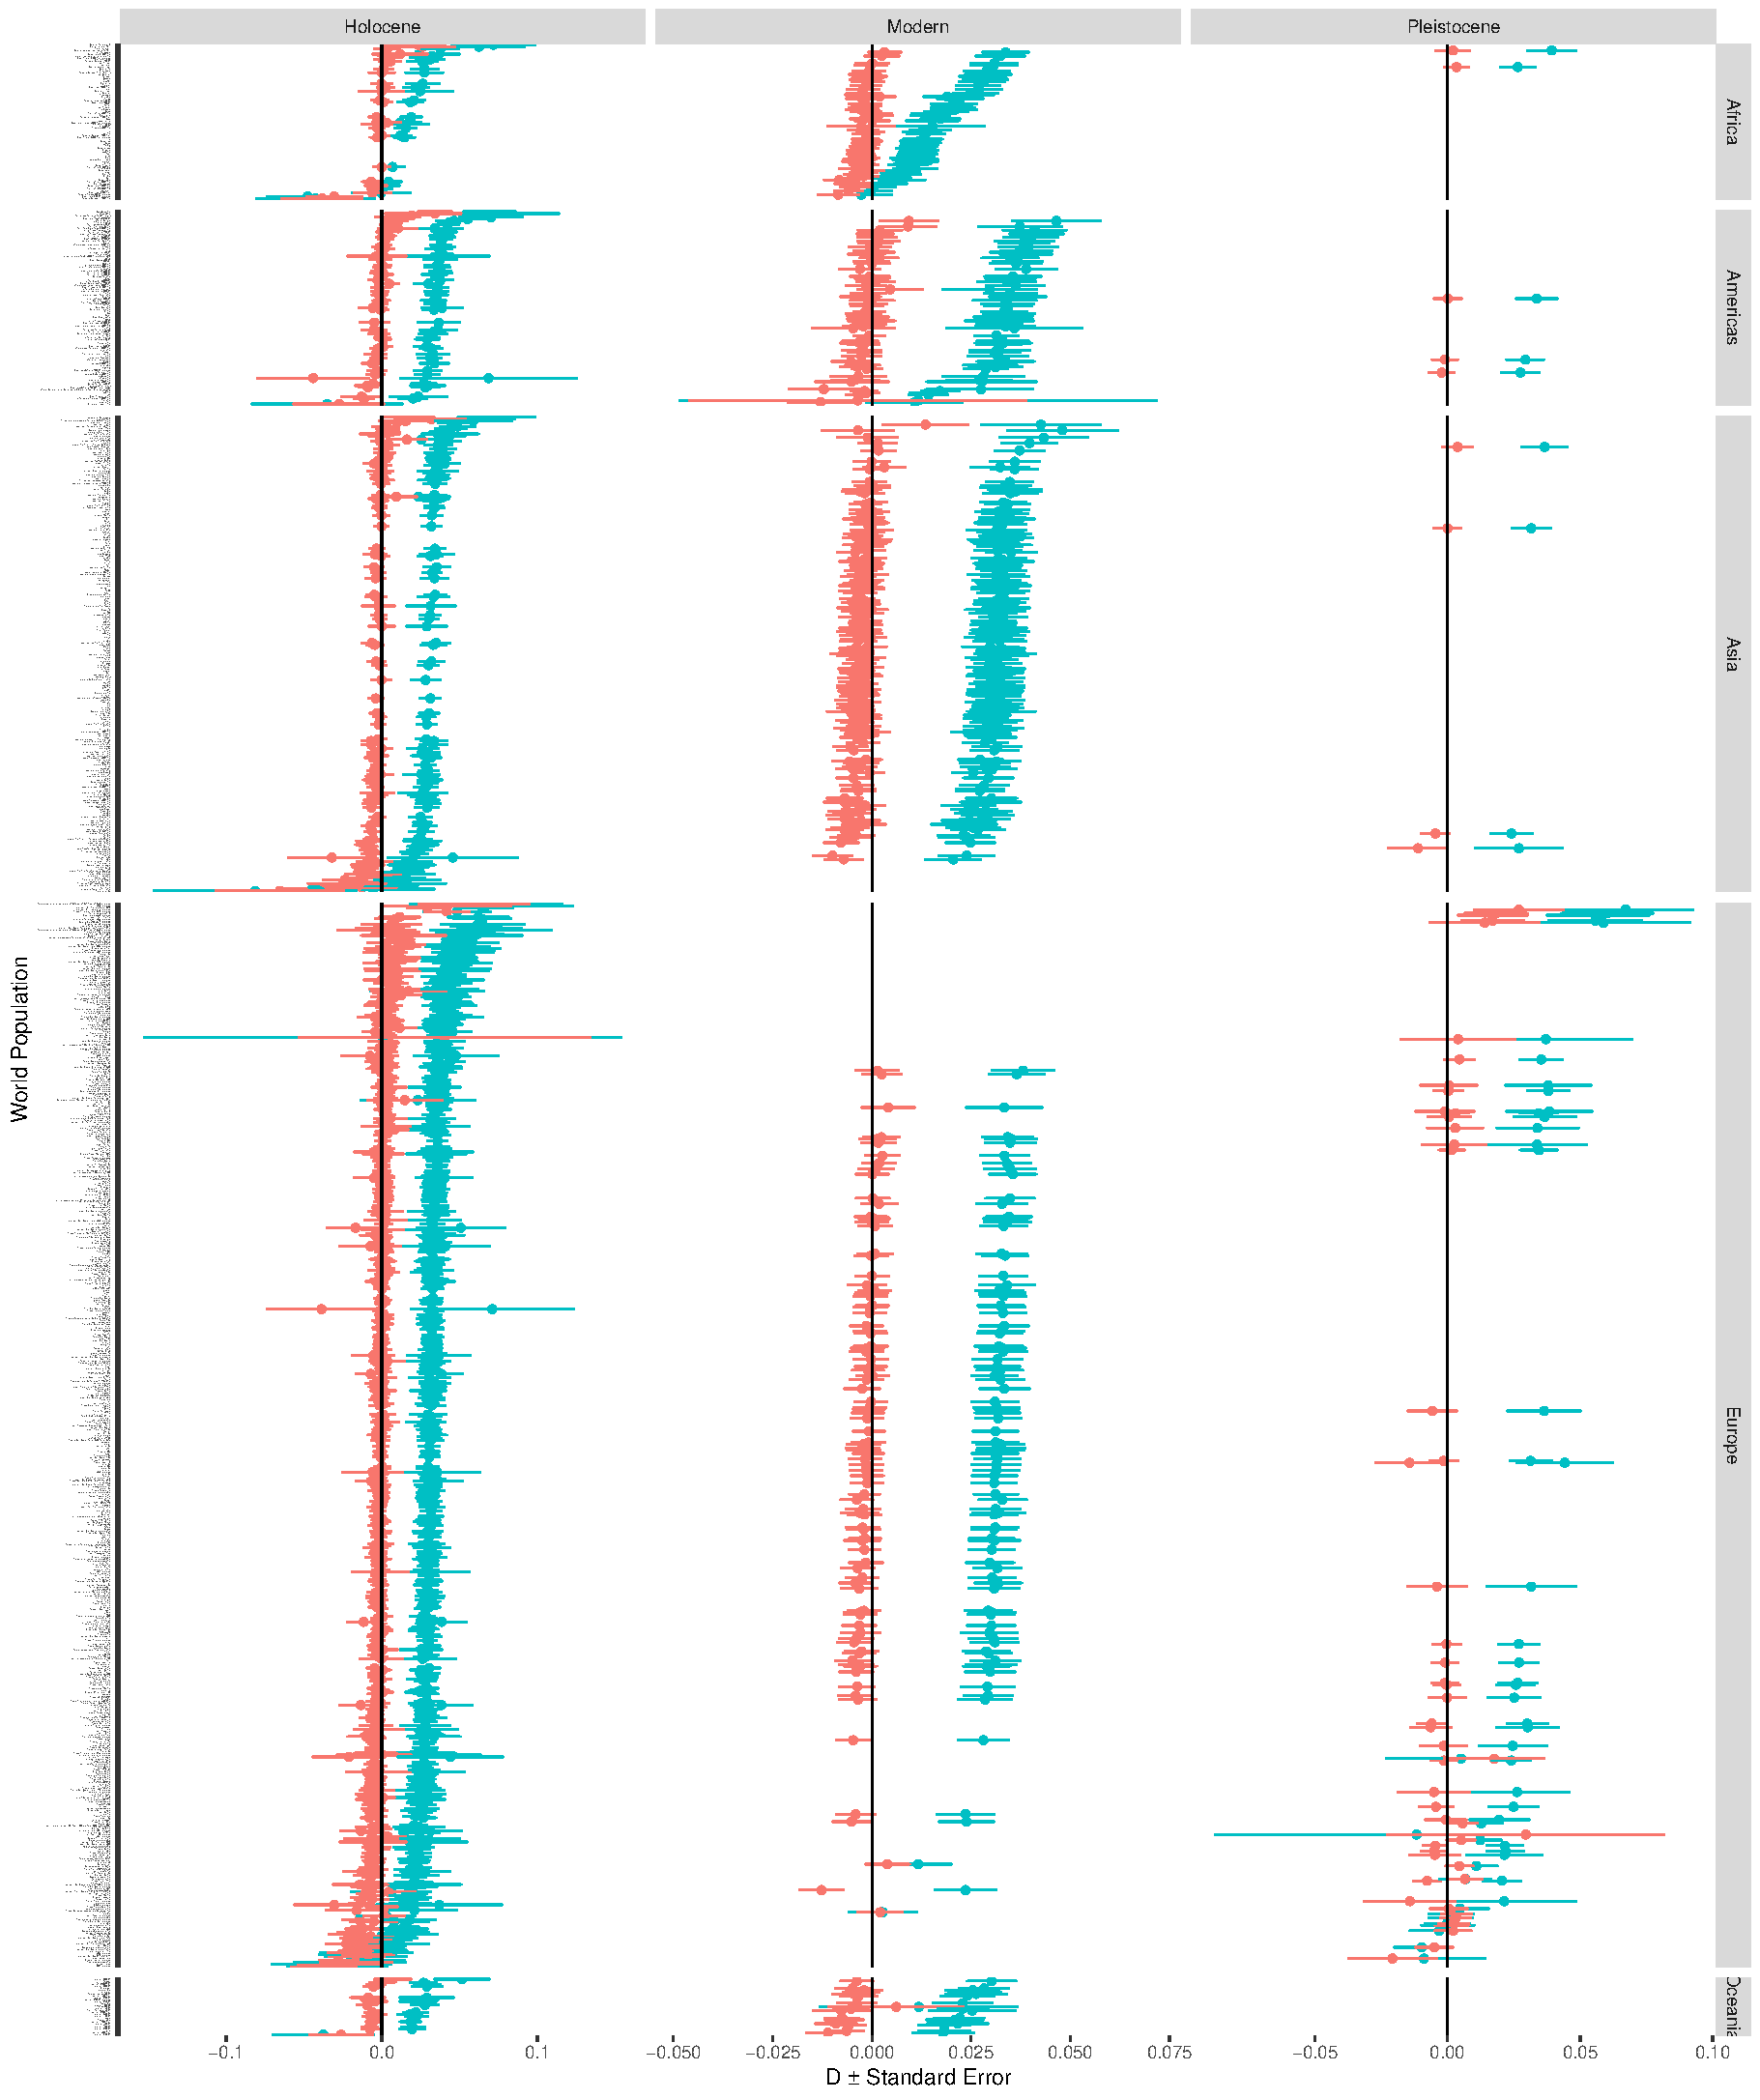
\includegraphics[width=\textwidth]{../plot/yri_d_stats.pdf}
	\caption{D statistics of the form (X, Chimp; Yoruba-1, Yoruba-2) for all global populations in the Human Origins dataset.}
	\label{fig:alld}
\end{figure}

\clearpage

\section{Simulation procedure} \label{simproc}

The ability of {\tt smcsmc} to recover a back-migration signal is evaluated through simulation. One gigabase of sequence was simulated in {\tt scrm}, and subsequently re-inferred by {\tt smcsmc}. Migration is parameterised by three factors, magnitude, midpoint, and duration. A scenario is simulated where the midpoint is the center of a block of a given duration which has uniform migration which integrates to a given total proportion replacement over the period. We use the following demographic model for population size throughout all simulations:

\begin{figure}
    \centering
    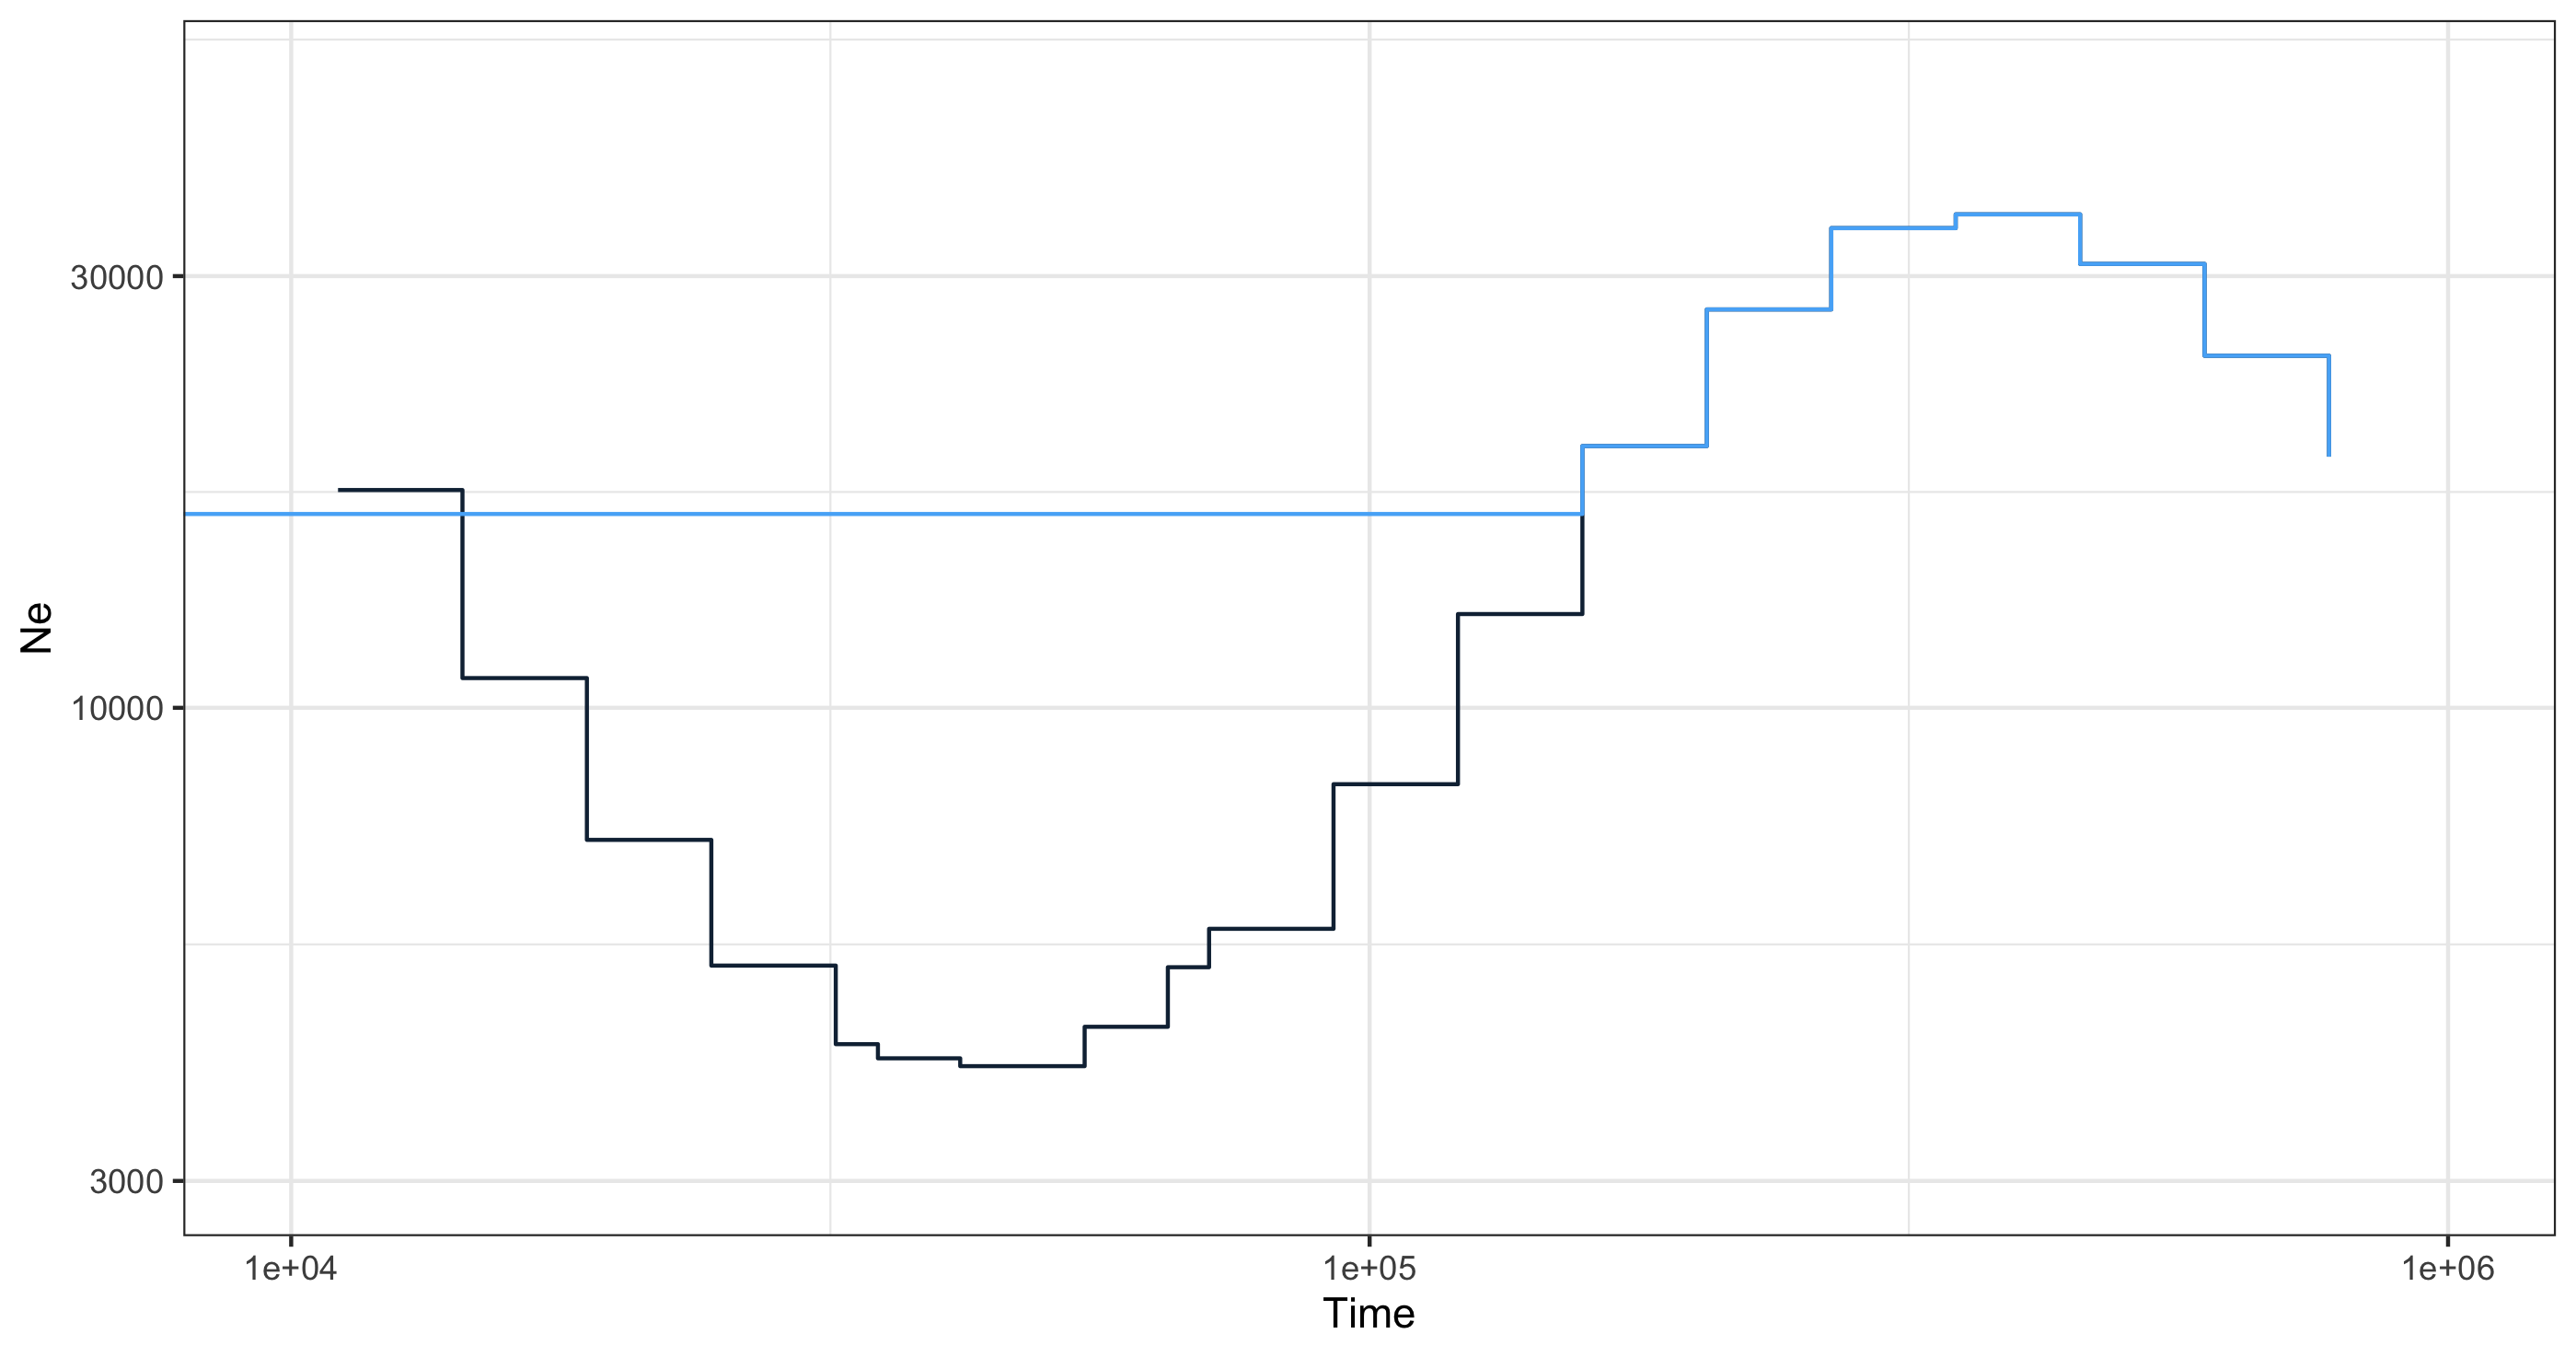
\includegraphics[width = 0.5\linewidth]{../plot/demographic_model.png}
    \caption{Population size model used for simulations.}
    \label{fig:dem}
\end{figure}



The following commands can be used in either {\tt ms} or {\tt SCRM} to specify demographic models. The African population size is given by 

\begin{verbatim}
-en 0.00000000 1 36.9124479 -en 0.00229999 1 14.8978177 -en 0.00299994 1 7.04453213 
-en 0.00391291 1 3.68961222 -en 0.00510371 1 2.06587476 -en 0.00665692 1 1.21617010
-en 0.00868280 1 0.75362392 -en 0.01132521 1 0.49927968 -en 0.01477178 1 0.36258332
-en 0.01926724 1 0.29687253 -en 0.02108190 1 0.28637149 -en 0.02513079 1 0.28071694
-en 0.03277878 1 0.31028768 -en 0.03915210 1 0.36107482 -en 0.04275426 1 0.39815181
-en 0.05576555 1 0.57528787 -en 0.07273654 1 0.88701054 -en 0.09487226 1 1.36014053
-en 0.12374449 1 1.92573639 -en 0.16140334 1 2.36832894 -en 0.21052280 1 2.45284038
-en 0.27459066 1 2.16222564 -en 0.35815613 1 1.71146032 -en 0.46715286 1 1.32388966
-en 0.60932028 1 1.09778746 -en 0.79475315 1 1.04669123 -en 1.03661833 1 1.16969768
-en 1.35208972 1 1.45788656 -en 1.76356769 1 1.80077313 -en 2.30026970 1 1.89942369
\end{verbatim}

While the European population size is given by

\begin{verbatim}
-en 0.00000000 2 1.14422216 -en 0.00229999 2 1.14422216 -en 0.00299994 2 1.14422216
-en 0.00391291 2 1.14422216 -en 0.00510371 2 1.14422216 -en 0.00665692 2 1.14422216
-en 0.00868280 2 1.14422216 -en 0.01132521 2 1.14422216 -en 0.01477178 2 1.14422216
-en 0.01926724 2 1.14422216 -en 0.02108190 2 1.14422216 -en 0.02513079 2 1.14422216
-en 0.03277878 2 1.14422216 -en 0.03915210 2 1.14422216 -en 0.04275426 2 1.14422216
-en 0.05576555 2 1.14422216 -en 0.07273654 2 1.14422216 -en 0.09487226 2 1.36014053
-en 0.12374449 2 1.92573639 -en 0.16140334 2 2.36832894 -en 0.21052280 2 2.45284038 
-en 0.27459066 2 2.16222564 -en 0.35815613 2 1.71146032 -en 0.46715286 2 1.32388966
-en 0.60932028 2 1.09778746 -en 0.79475315 2 1.04669123 -en 1.03661833 2 1.16969768
-en 1.35208972 2 1.45788656 -en 1.76356769 2 1.80077313 -en 2.30026970 2 1.89942369
\end{verbatim}

Times are in units of $4gN_0$ while population sizes are in units of $N_0$. For $g=29, N_0 = 14312$, the demographic model is as shown in Supplemental Figure \ref{fig:dem}.  

The demographic model which we have assumed for both population's effective sizes has been shown to recapitulate similar inference to real data (data not shown). The migration parameter must be initiated at a given magnitude; further back in time, the particle filter is less able to identify lineage's true populations, and the inference of migration rates becomes essential uniform. Thus, we see a ``drop-off'' effect, where in the ancient past, the inference remains at the initiation value, and as more certainty about different histories is obtained, the migration values recapitulate real information. Thus the choice of an appropriate parameter for the initial migration rate is a crucial step in {\tt smcsmc} analysis, and here we chose to arrive at this value through simulation.

We simulate back-migration scenarios of varying total migration proportions from 0 (no migration) up to 60\% population replacement.For each simulation, we initiate the particle filter at either 0, 1, or 5 4$N_0$ proportion replaced per generation (which are the units used internally by {\tt scrm} and {\tt ms} for simulation).  {\tt smcsmc} is then used to infer effective population size and migration histories in five iterations with 5000 particles. As a cautionary note, these simulations are almost certainly not fully converged, and are used as an indication of power. Their power, theoretically, approaches 1, as particle filters asymptotically exactly approach the true posterior distribution. However, these low resolution attempts are indicative of a ``quick'' overview of the abilities of the algorithm. With 600 cores available, each of the cases (forward, backward, or bidirectional) was able to run in approximately 20 hours. 

Generally, beginning with a higher migration rate seems to recover a higher proportion of the simulated migration. However, as in the case of a 60\% replacement simulated 40kya, beginning with 5 4$N_0$ rather than 1 4$N_0$ recovers similar proportions of backwards migration (0.502 vs 0.52) yet the higher migration rate finds 0.301 Eurasian migration rather than 0.195. The higher initial migration rates thus slightly reduce power (though, not in all cases, and for fully converged solutions, we would expect both proportions to be similar up to noise) while additionally finding an increased migration in the opposite direction.  Beginning with a zero rate leads to highly unstable estimates of the migration rate and effective population size, and we exclude it from our analysis.

We select a more comprehensive set of initiation parameters and particle values and use them to analyze a Yoruban and French individual from SGDP (Fig \ref{init_yri}). The effect of the initial migration rate seems relatively consistent for low values (0.5 - 2.0),while an increasingly small migration peak is seen for higher initial magnitudes 4.0 - 10.0. Again, beginning with an initial rate of zero tends to lead to highly unstable estimates of effective population size and migration rates. For the remainder of the analyses in this article, we choose to use an initial rate of 1.0. 


\begin{figure}
	\centering
	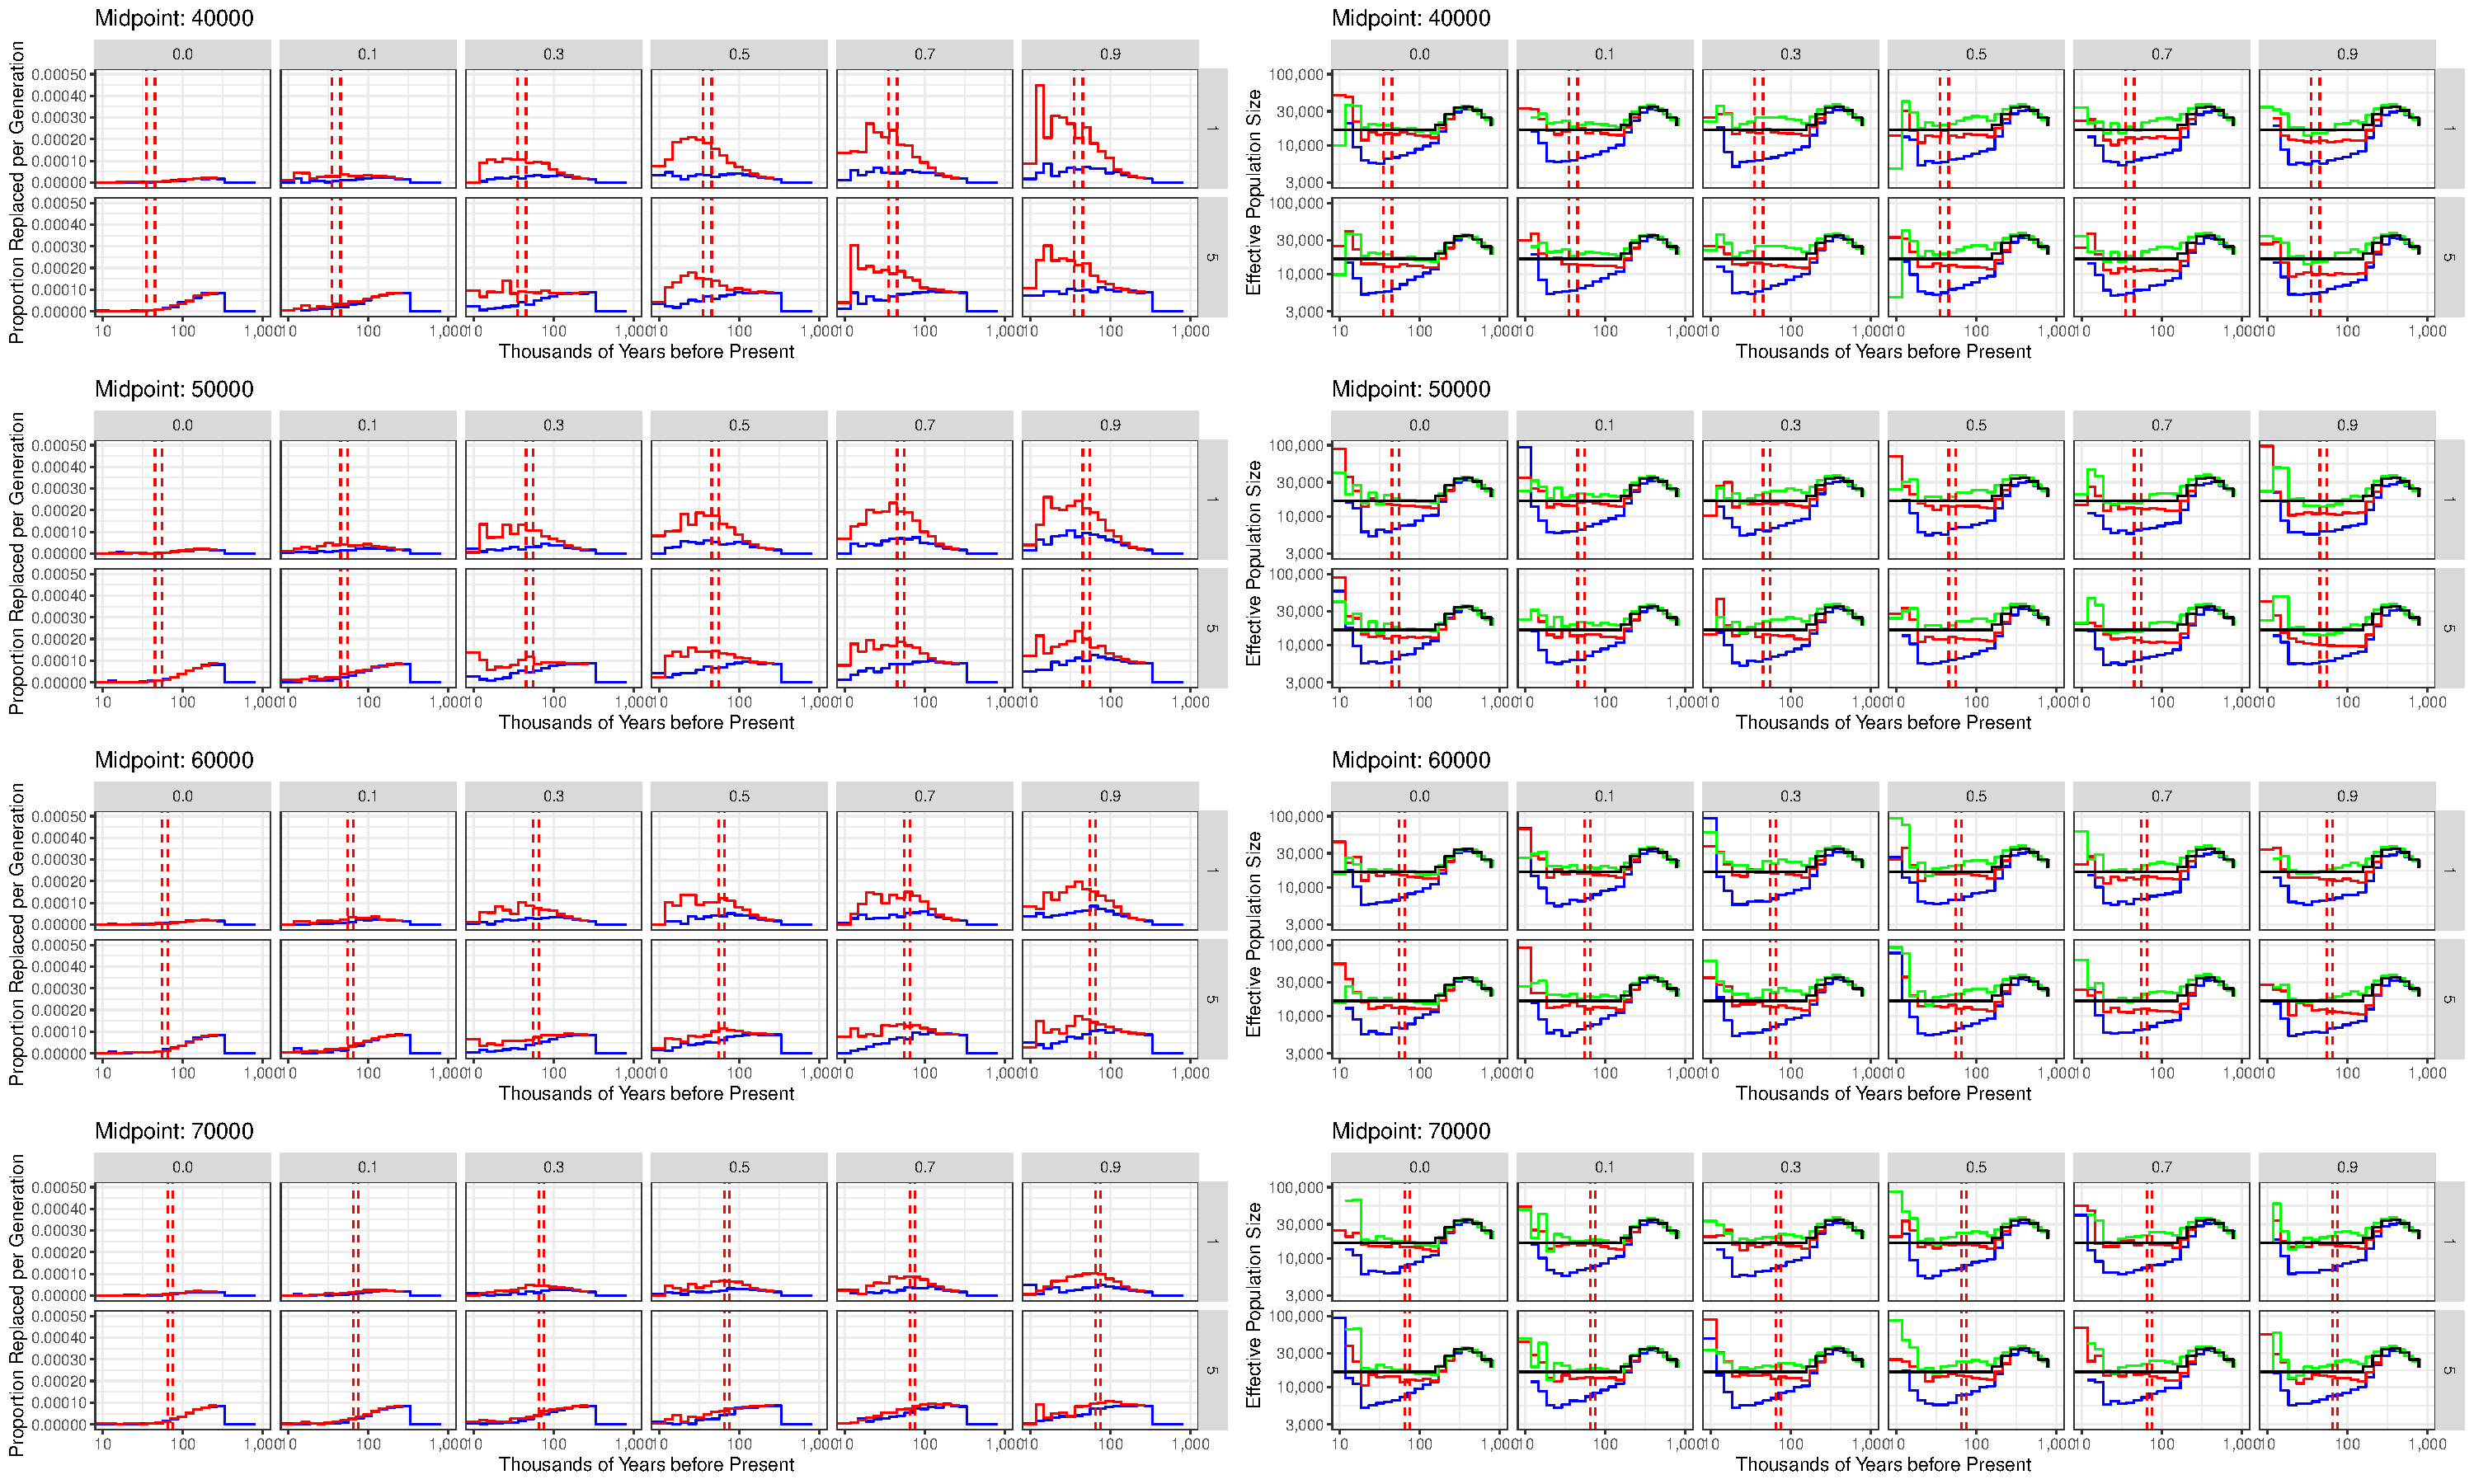
\includegraphics[width=\textwidth]{../plot/sims/backward_different_starts.pdf}
	\caption{Backwards simulation}
	\label{fig:backsim}
\end{figure}


\begin{figure}
	\centering
	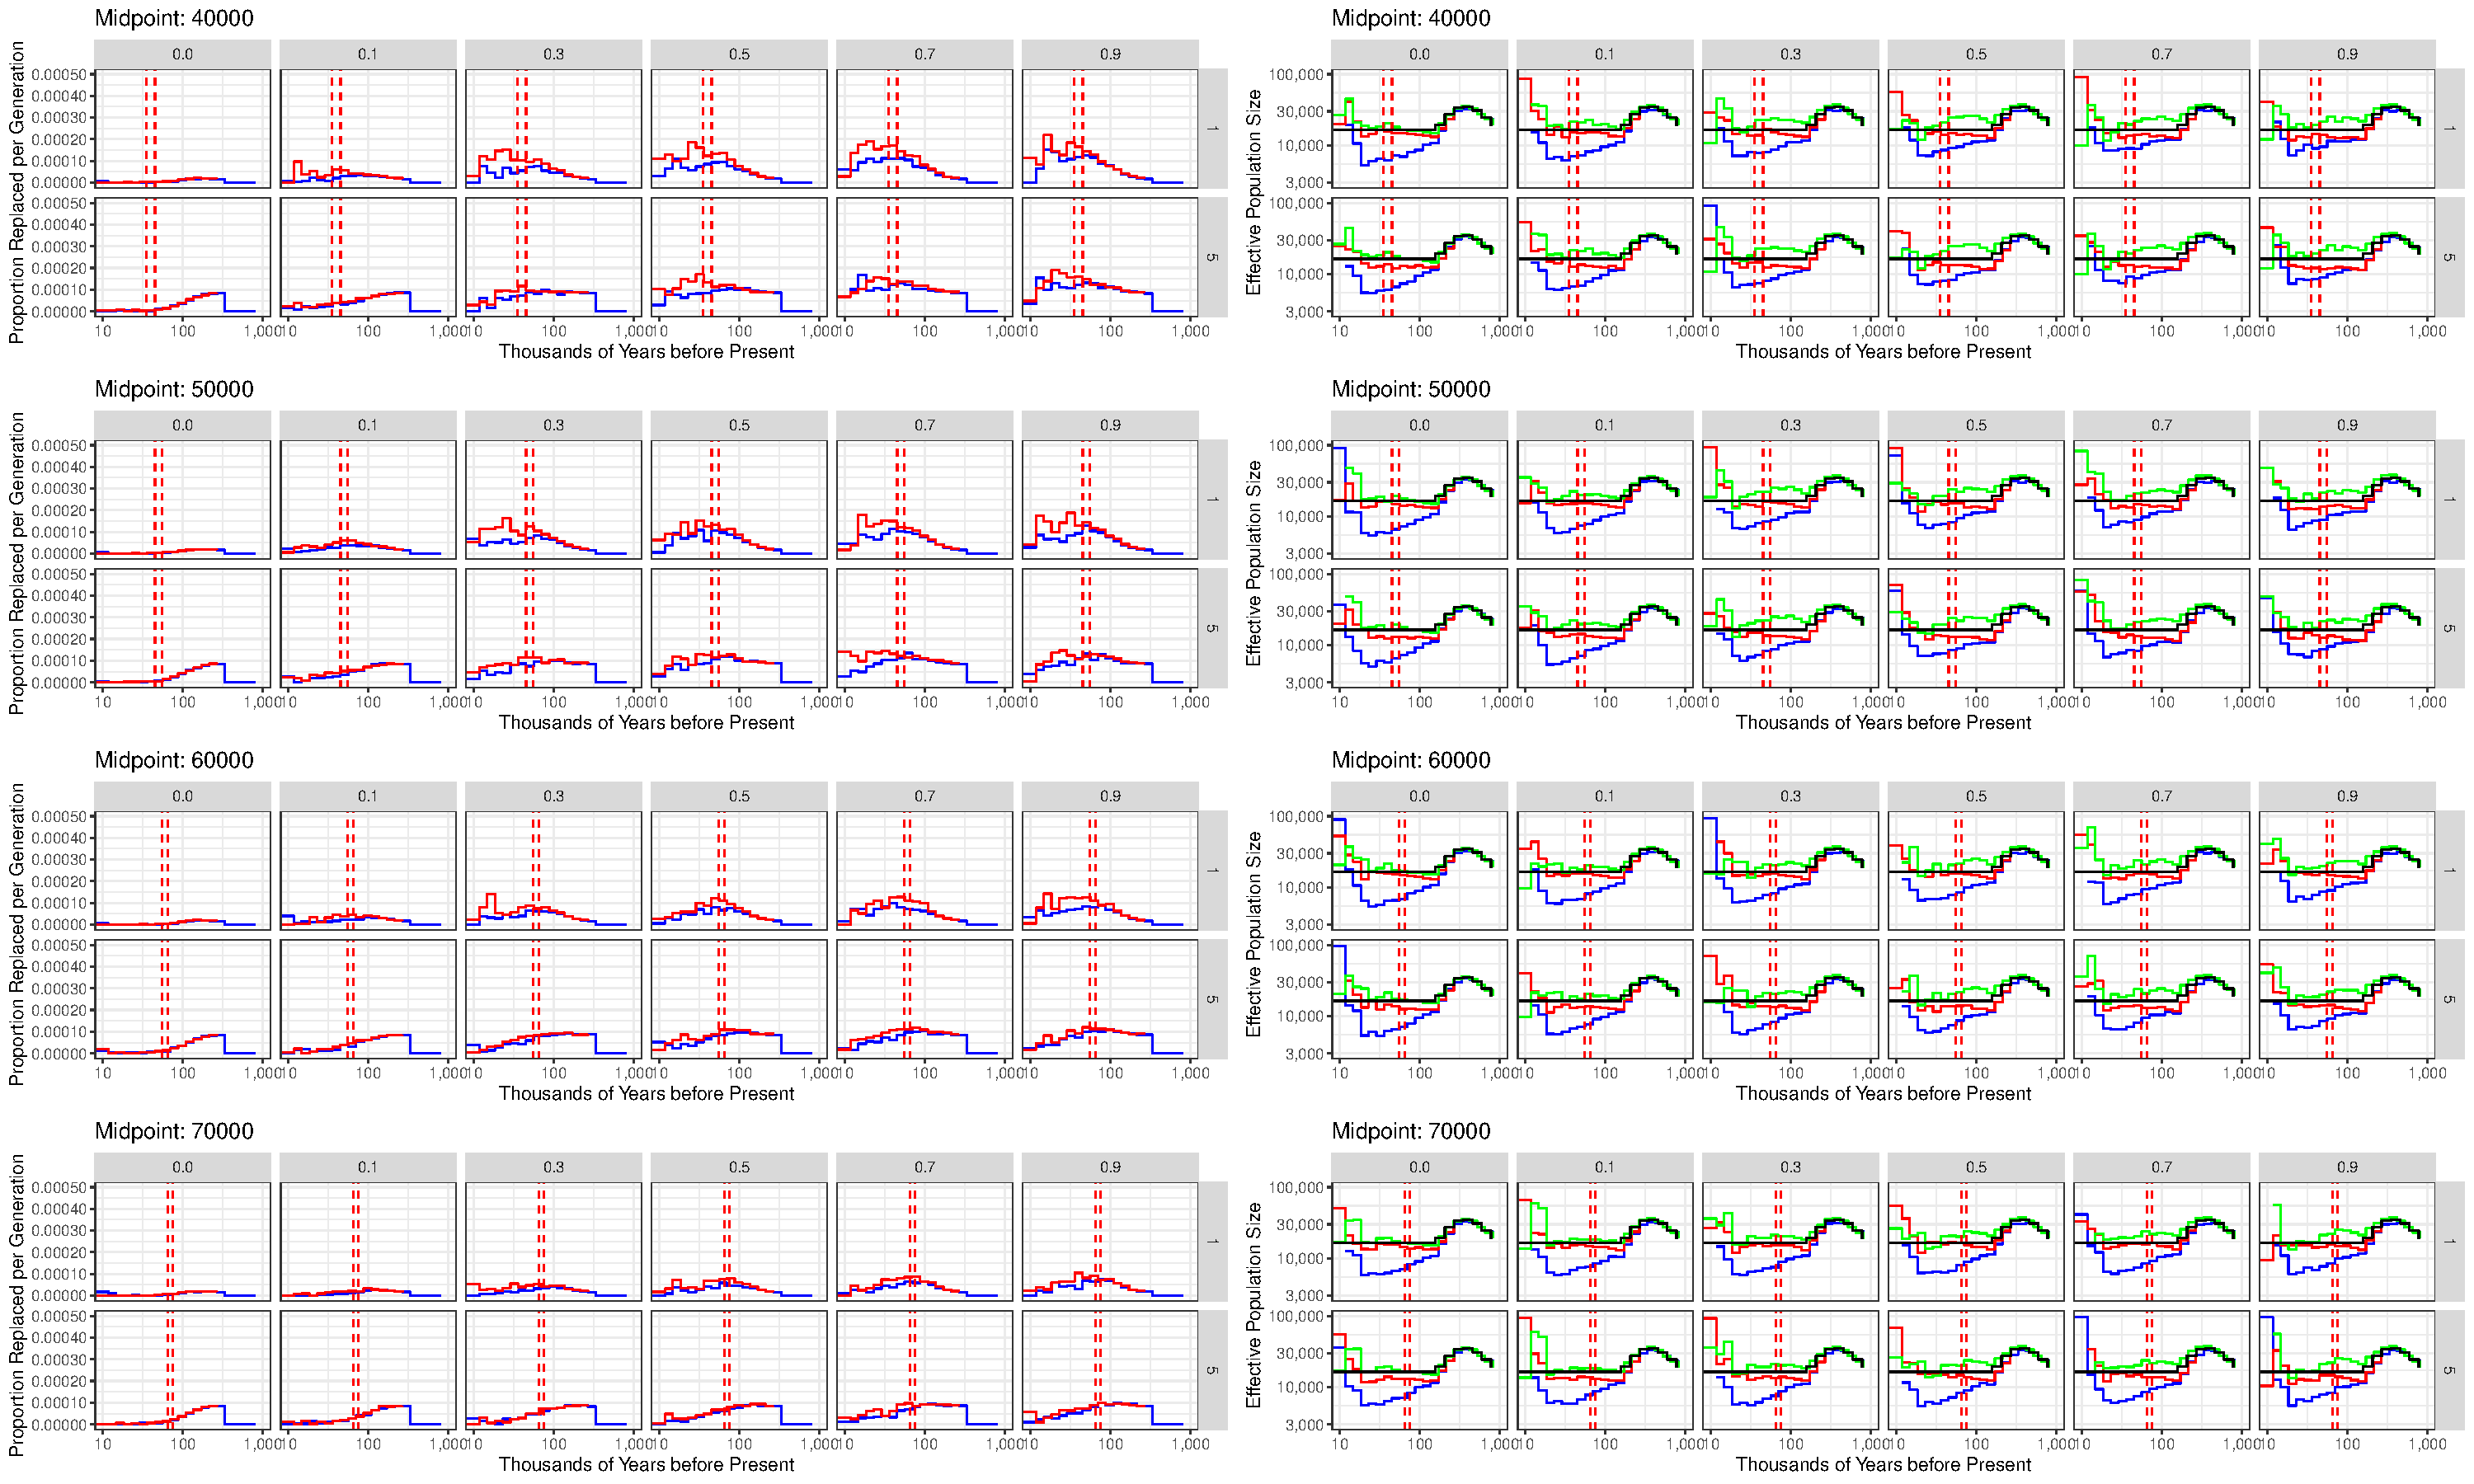
\includegraphics[width=\textwidth]{../plot/sims/bidirectional_different_starts.pdf}
	\caption{Bidirectional simulation}
	\label{fig:bisim}
\end{figure}

\begin{figure}
	\centering
	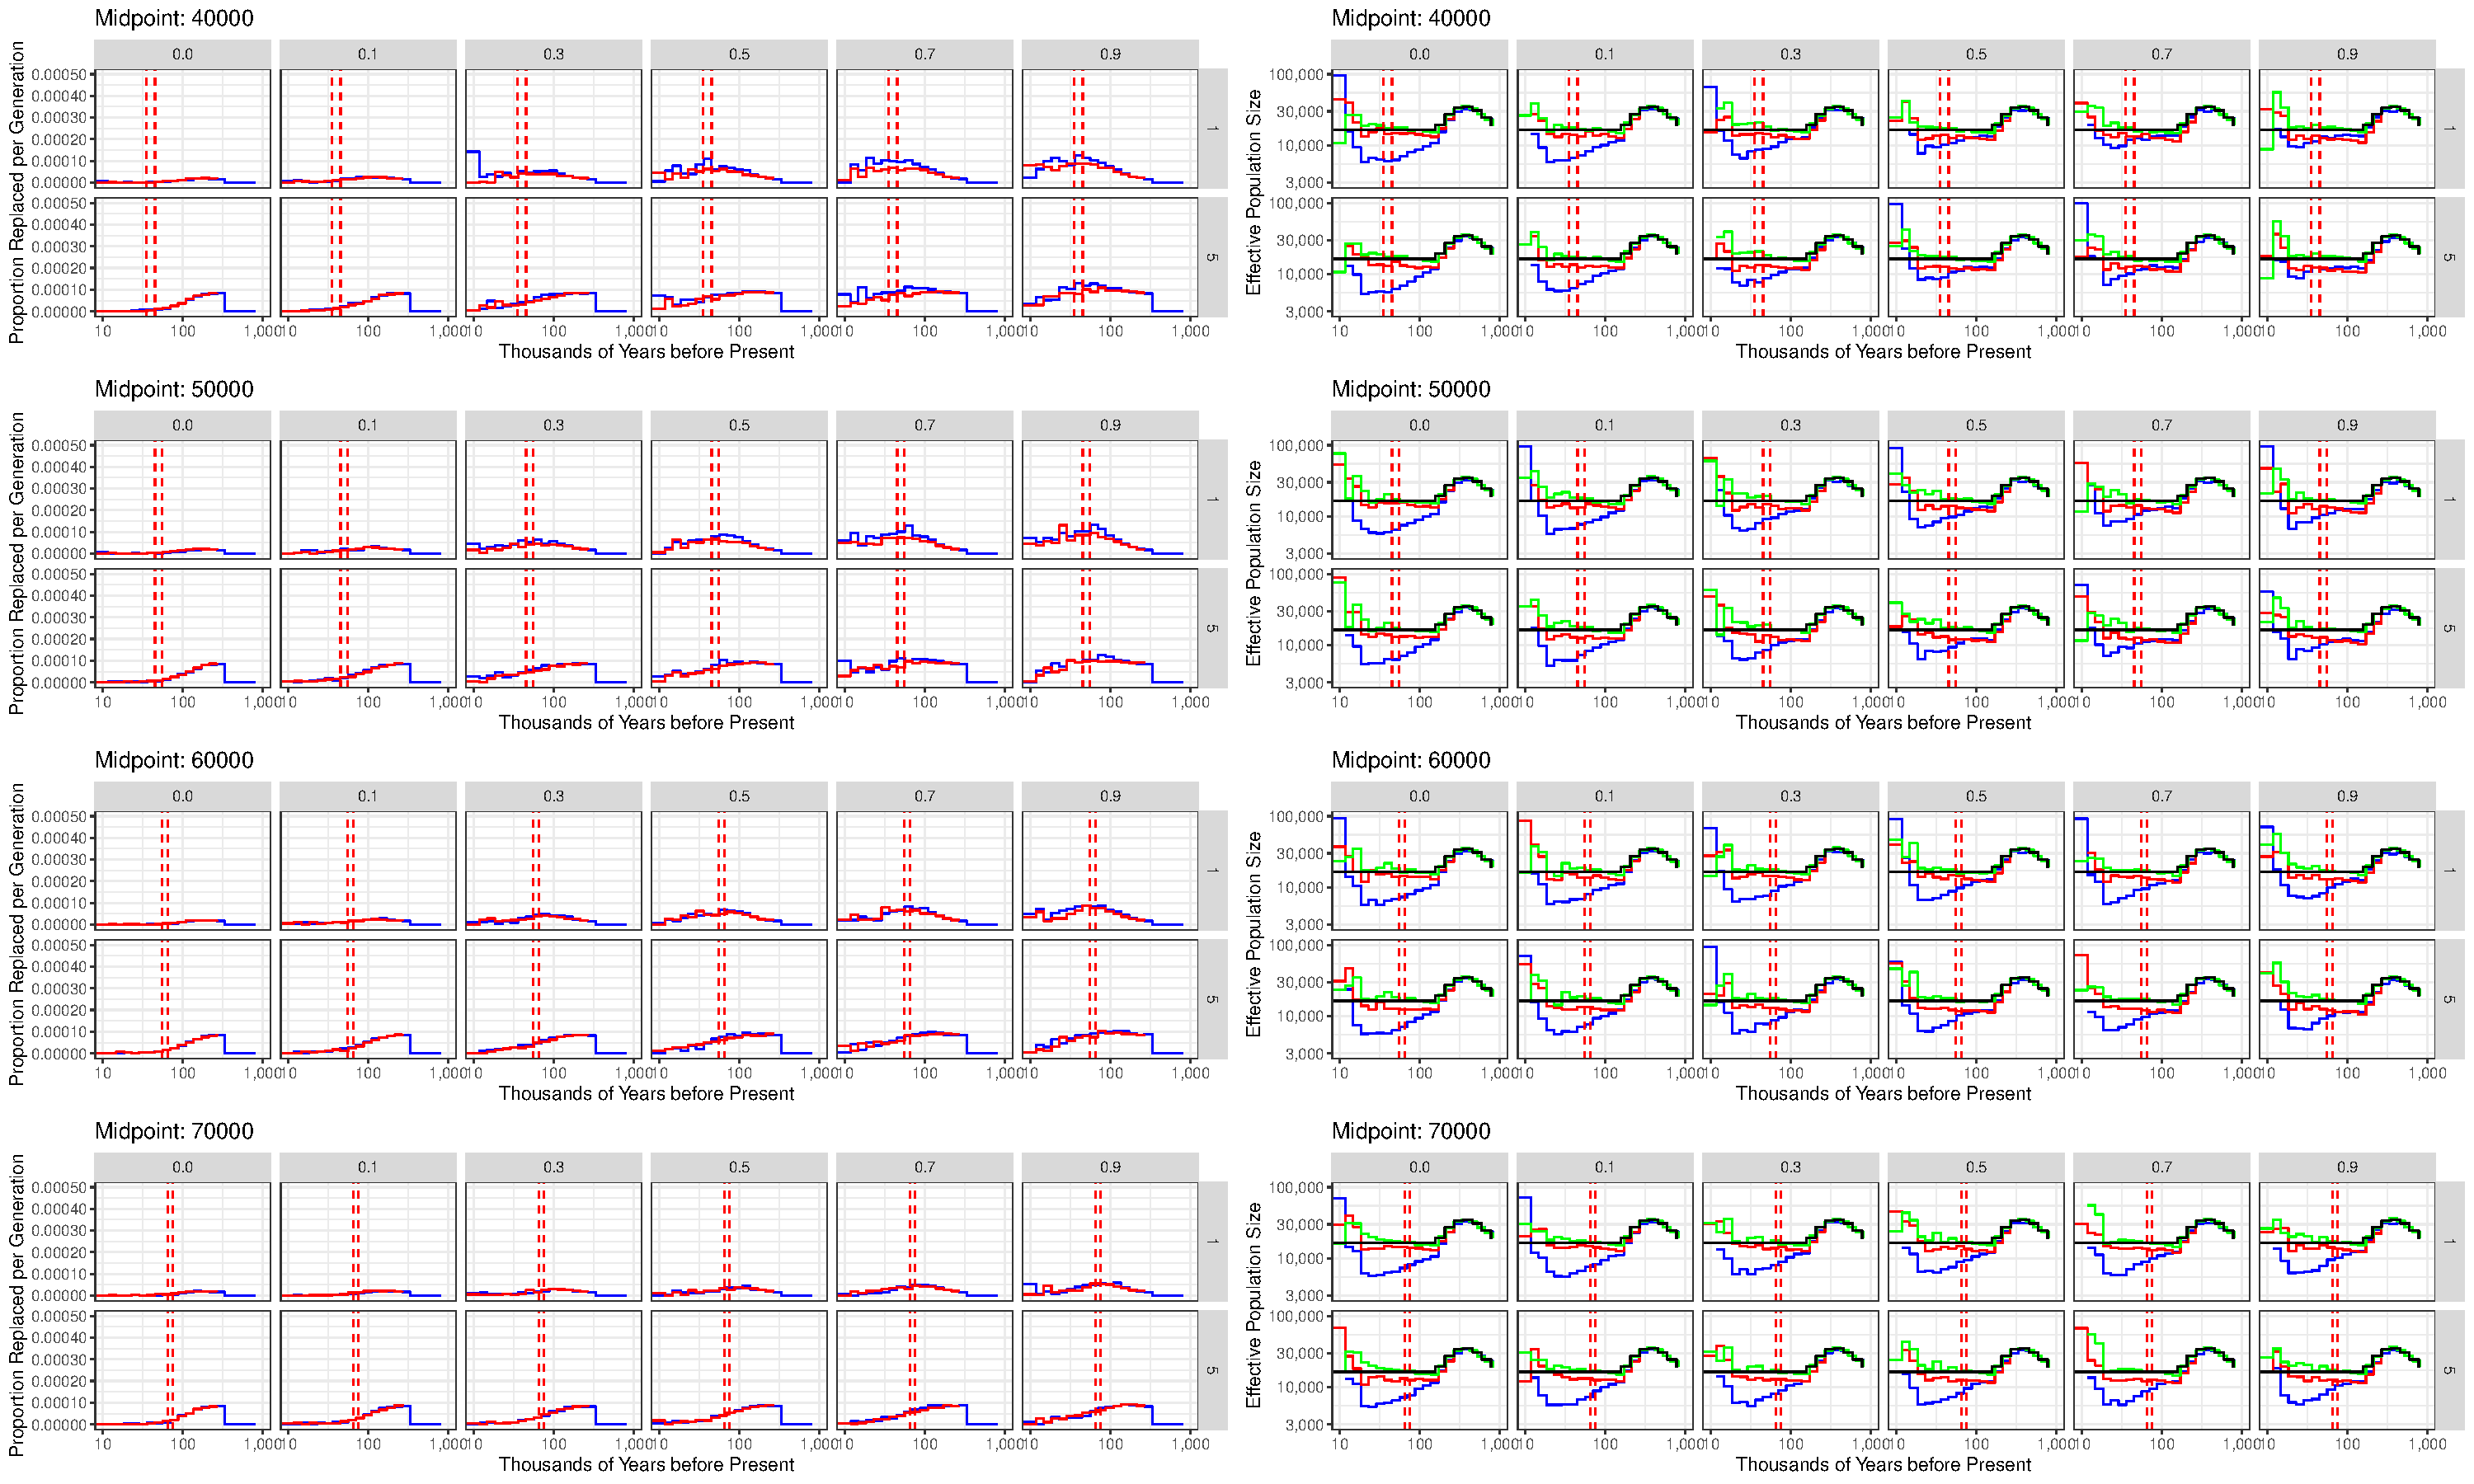
\includegraphics[width=\textwidth]{../plot/sims/forward_different_starts.pdf}
	\caption{Forward simulation}
	\label{fig:fwdsim}
\end{figure}


\begin{figure}
	\centering
	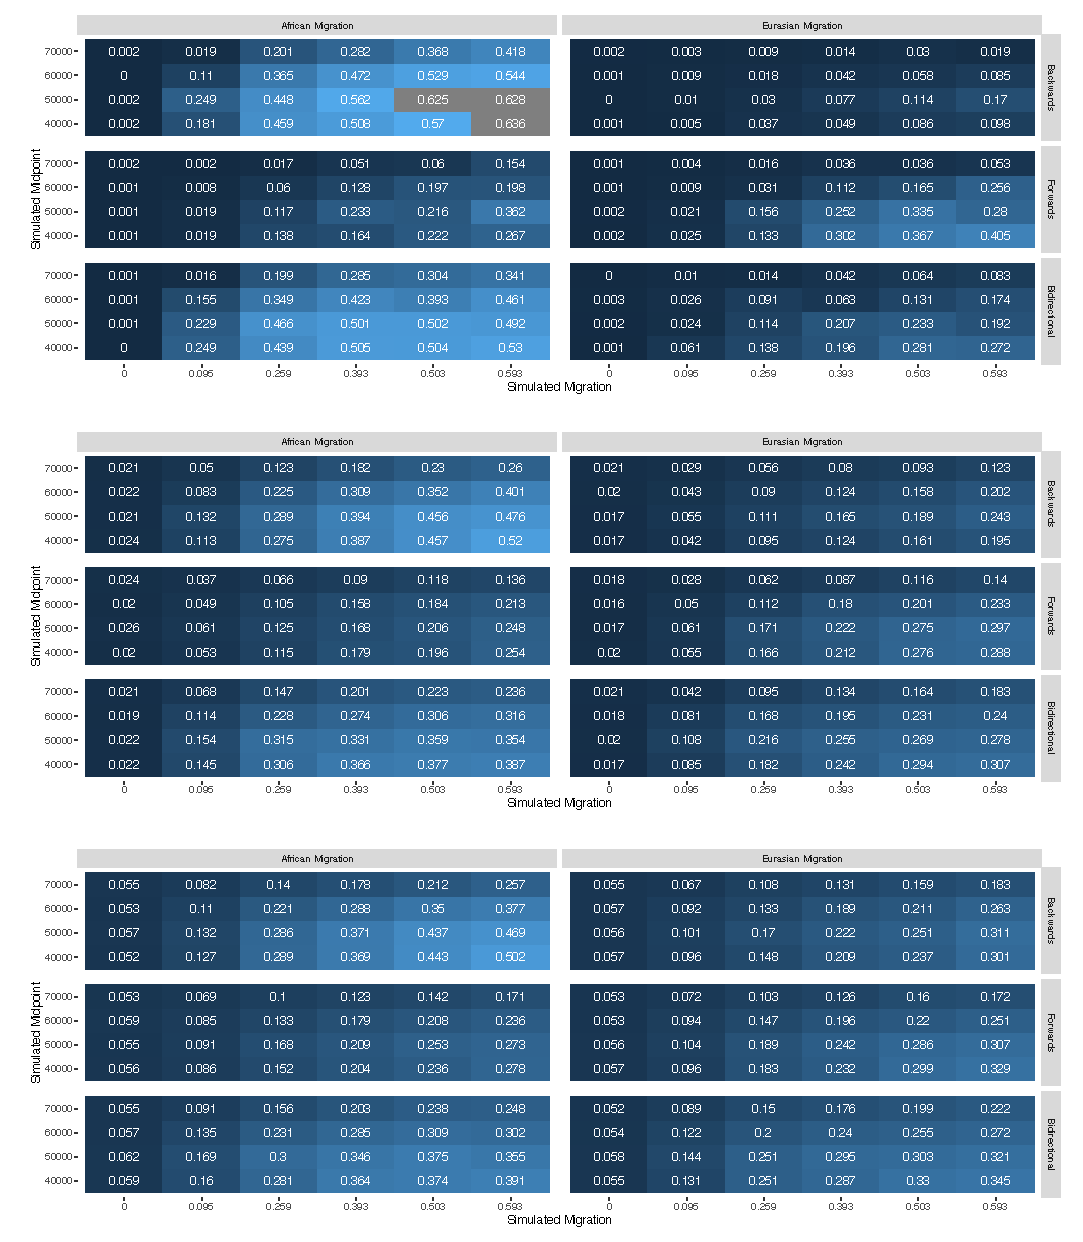
\includegraphics[width=\textwidth]{../plot/sims/all_integrated_sims.pdf}
	\caption{Area under the migration curve for three cases of simulated demography shown in Figures \ref{fig:backsim}, \ref{fig:bisim}, and \ref{fig:fwdsim}. From top to bottom, inference was initiated with 0, 1, and 5 4$N_0$ population replacement per generation.}
	\label{fig:intsim}
\end{figure}


%\begin{figure}
%	\centering
%	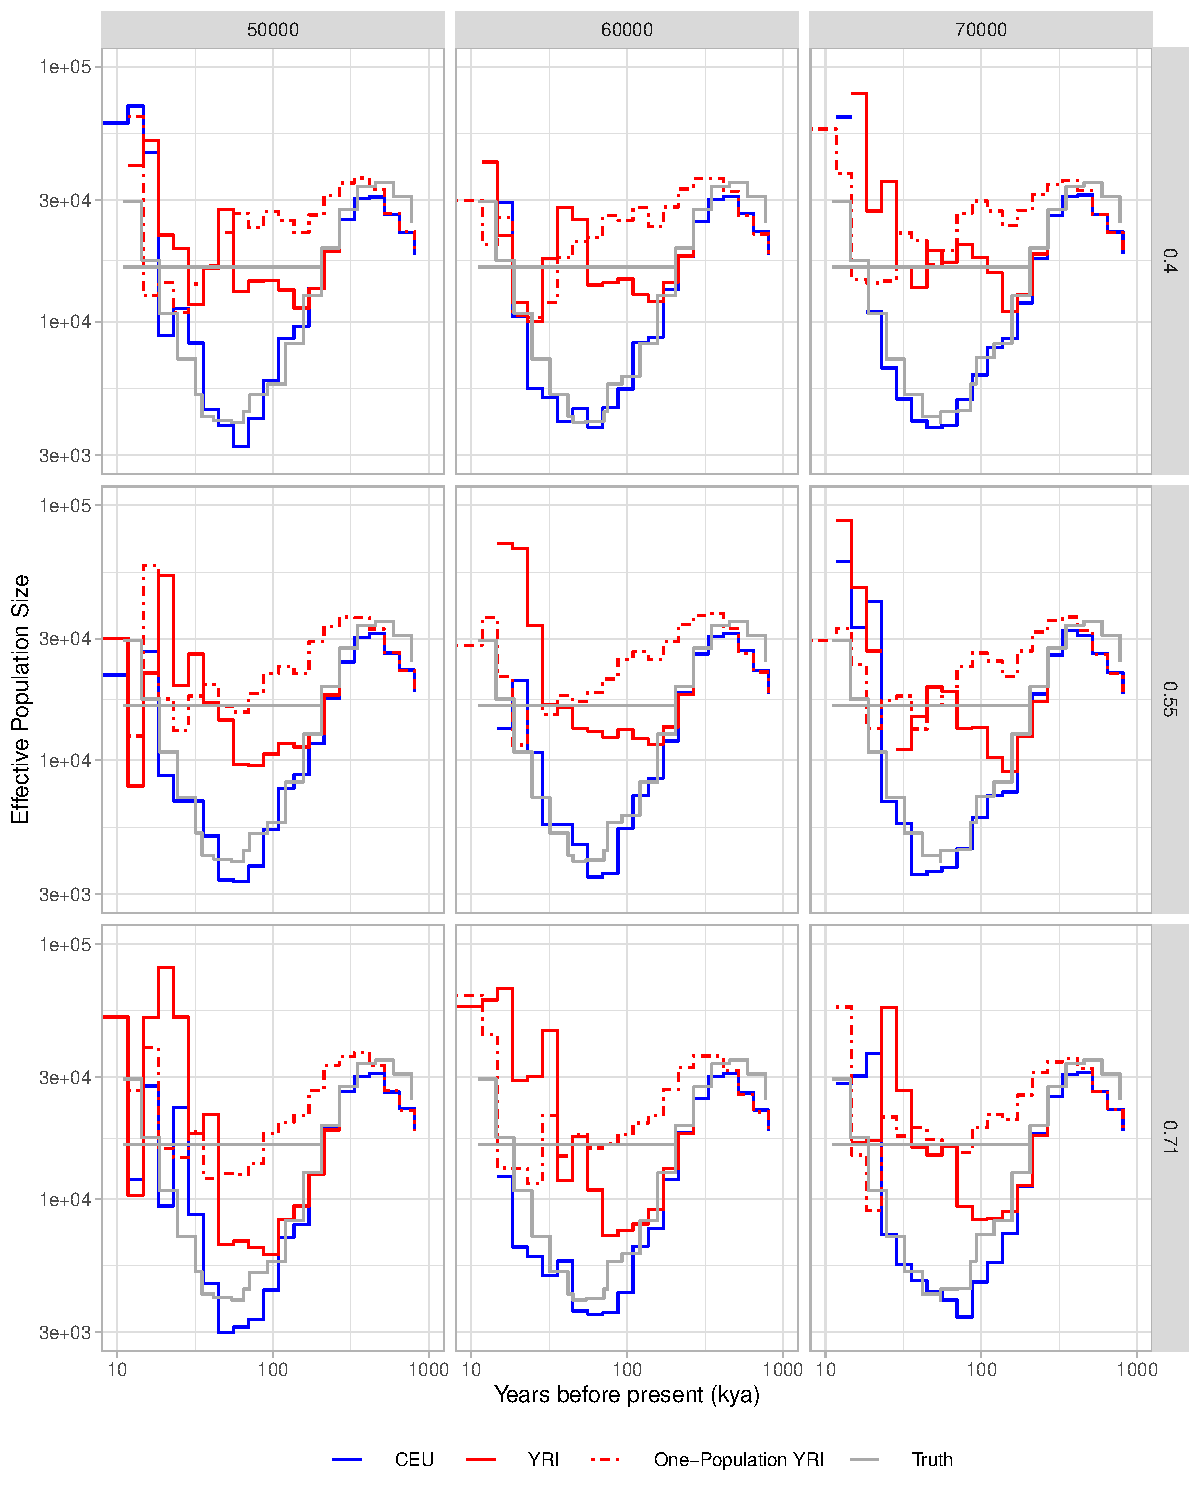
\includegraphics[width=0.5\textwidth]{../plot/old_all_li_durbin.pdf}
%	\caption{Simulated directional migration from effective ``African'' to ``Eurasian'' populations. For this figure, duration of the migration was fixed at 10ky. Simulations performed in {\tt scrm} with one gigabase of sequence. Inference performed in {\tt smcsmc} with five iterations of variational Bayes and 5000 particles.}
%	\label{nesims_10ky}
%\end{figure}

% old intro

%The early population structure of anatomically modern humans (AMHs) in Africa and their eventual migration into the Eurasian continent have shaped global patterns of genetic variation \cite{Pagani2016, Nielsen2017a}. However, little is known about population structure within Africa prior to the expansion of agriculturalists and pastoral groups \cite{Busby2016, Patin2017}. Recent evidence from the handful of successfully sequenced ancient African genomes hint at large-scale population movements and admixture from multiple highly divergent, extinct populations, with complex affinities to current groups \cite{Skoglund2018, Lipson2019, GallegoLlorente2015a}. The majority of structure in the continent is derived from events in the Holocene, including the spread of Bantu languages from Western Central Africa both East and South, as well as admixture from pastoralists its in the Near East and Western Eurasia \cite{Busby2016}. Eastern Africans are the most closely related group to the ancestral Out of Africa migrants, though they show particularly high levels of ancestry related to neolithic populations from Iran and the Levant consistent with multiple waves of back-migration in the Holocene \cite{Skoglund2017}.  Evidence for recent admixture from Eurasian sources is well established, however the lack of ancient African DNA from the Pleistocene has confounded efforts to uncover interactions between the earliest inhabitants of the continent. While the migration event associated with establishing current global population structure has been confidently dated between 60-80kya, Central and South African hunter gatherers such as the Mbuti and KhoeSan (without implying linguistic unity, defined as southern African hunter gatherers who speak non-Bantu languages which include a click consonant) may have diverged from other groups 200-250 thousand years ago (kya) \cite{Lipson2019, Schlebusch2017}. In the intervening millennia, fossils identified as AMH have been found in China about 80-120kya, Sumatra about 63-73kya, and artifacts from Australia 65kya \cite{Clarkson2017, Liu2015, Westaway2017}. Support for multiple migrations across Eurasia additionally comes from climate science, where four distinct periods of warming may have provided vegetated migration routes out of Africa (OoA) as early as 120kya \cite{Timmermann2016}. The extent of contributions to modern day populations from ``ghost'' populations is unknown, though controversially suggested in Australasia and South East Asia \cite{Malaspinas2016, Mallick2016, Pagani2016, Rasmussen2011, Skoglund2015} and Africa  \cite{Durvasula2019, Speidel2019, Lipson2019, Hammer2011, Plagnol2006, Ragsdale2019}. To a large degree, the fate of these anciently diverged populations and their contributions, if any, to modern day populations remains an open question. Here, we apply a recently developed particle filter using the sequentially Markovian approximation of the coalescent with recombination to dissect historical directional migration in Africa \cite{Henderson2018}. 

%\todo[inline]{Question: Do you think that we need a review of other methods here? Do we need to defend our choice to use smcsmc?}

%Little is known about population structure within the African continent Current evidence mostly supports an early diversification of both Central and South African hunter gatherers, though the order is not yet resolved, possibly up to 200-250kya. \cite{Lipson2019,Schlebusch2017, Skoglund2017} The divergence between African and Out of Africa (OoA) lineages has been robustly dated to between 60 and 80kya, supported by both whole genome demographic inference and mtDNA phylogeography \cite{Lipson2019,Soares2012}. In the intervening millennia, archaeological evidence supports AMHs inhabiting sites in China, Australia, and Sumatra before the main OoA event \cite{Clarkson2017, Liu2015, Westaway2017}. The fate of these earlier migrants and their contribution to modern day populations remain an open question. 

%Unsampled populations, sometimes referred to as ``ghost'' populations, have been suggested to contribute to several global populations, most notably and controversially in Australasia and South East Asia . However, recent evidence points towards large unexplained patterns of admixture from both ancient and modern populations to several groups in Africa \cite{Durvasula2019, Lipson2019, Skoglund2017, Hammer2011, Plagnol2006, Ragsdale2019}. Support for these admixture events mainly derives from inference under approximations of the coalescent with recombination, analysing the site frequency spectrum, and fitting expectations of drift statistics to observed quantities. However, to date an understanding of the magnitude and timing of these migration events has been confounded by a lack of appropriate statistical methods for inferring directional migration over a wide range of time. 

%Approximating the coalescent with recombination with a Markovian process along the genome has provided a tractable framework for the inference of effective population size \cite{McVean2005}. Recent applications have adopted the sequentially Markovian coalescent (SMC) and its derivatives for inference in up to eight haploid individuals in methods such as the pairwise and multiple SMC (PSMC and MSMC) \cite{Li2011, Schiffels2014}. MSMC additionally infers a cross-population coalescent rate, which can be scaled to reflect relative symmetrical gene flow. Both methods estimate $N_e$ as the scaled inverse of the coalescent rate, a quantity which is equivalent to effective population size in panmictic populations but not in the presence of structure \cite{Chikhi2018}. Here, we use a newly developed particle filter to simultaneously estimate both $N_e$ and directional migration in up to eight haploid individuals, and explore population structure in the ancient past. A combination of importance sampling and a resampling process guided by a novel lookahead-likelihood samples from the posterior distribution of piecewise constant geneological trees collectively called the ancestral recombination graph (ARG). Variational Bayesian inference is used to estimate, in theory any demographic parameter which admits simulation along the sequence, but in practice effective population size and directional migration rates.  



% old results
%One individual was selected from each of the African populations in the Simons Genome Diversity Panel and their effective population size was modelled along with three seperate partner populations (French, Han Chinese, and Papuan) using both {\tt smcsmc} and MSMC (Figure \ref{neplot}). Directional migration rates between the African and Eurasian populations are simultaneously estimated; the converged parameter estimates represent the most likely set of piecewise constant parameter values. We choose to infer parameter values over 31 epochs equally spaced on the log scale. The inference of population size with MSMC and {\tt smcsmc} is mostly consistent, especially for the estimation of the Eurasian $N_e$ (blue in Figure \ref{neplot}). Both algorithms identify a clear bottleneck and subsequent expansion associated with the Out of Africa event. However, the estimation of African population size differs. In the ancient past, prior to the OoA event, MSMC identifies an early split between the two populations, followed by a transient increase in the African $N_e$ up to an average of approximately 40,000 individuals before coming back down to a stable estimate (red in Figure \ref{neplot}, detail in Figure \ref{averages}). This contrasts with the inference from {\tt smcsmc}. In all populations, there is no inflation in the African $N_e$ relative to the Eurasian one prior to population divergence, and the split times are additionally delayed, bringing them more in line with current estimates. A smaller ancestral African population size is inferred in each individual averaged over Eurasian donor (Figure \ref{averages}). We suspect that the differences in population size inference may be due to {\tt smcsmc} simultaneously accounting for directional migration. To test whether systematic differences in the inference methods may be responsible, a single population model is fit to two Yoruban genomes. When no migration parameters are fit, {\tt smcsmc} and MSMC infer very similar histories (green in Figure \ref{neplot}). To verify that systematic errors in the statistical phasing of the SGDP were not confounding inference, we performed the same analysis on 32 individuals from the Human Genome Diversity Panel whose genomes have been physically phased (Supplemental Section \ref{hgdp_section}). All trends identified in the SGDP are additionally present in the physically phased HGDP.   

%\todo[inline]{I haven't made plots for the HGDP analysis yet becuase the MSMC runs haven't finished.}

%A variety of demographic scenarios were simulated in {\tt scrm} to investigate the role of migration in population size inference. The timing of the migration, its duration, as well as the total proportion of the sink population replaced are varied systematically. Population size was inferred under a two island model with migration, performed similarly to the analysis of real data above. Additionally, the ``African'' genome in the analysis is isolated and modelled alone in a one-population analysis. A skeleton of Eurasian and African population size through time, given in Supplemental \ref{simproc}, is used as the truth in the simulations. Systematic underestimation of the African $N_e$ is found in the two-population analysis, while the $N_e$ is systematically inflated during the migration event and prior to population split in the single-population analysis (Figure \ref{sim}).  

%Examining the migration rates inferred by {\tt smcsmc} supports this hypothesis. In all populations studied, migration from Eurasia to Africa is higher than the reverse (Figure \ref{migrationplot}a). The choice of Out of Africa population significantly impacts the amount of migration inferred (Figure \ref{averages_of_sgdp}). In general, and in each specific language family, Papuans significantly contributed approximately 5 percent less (individual comparisons shown in Figure \ref{averages_of_sgdp}) to the ancestral African population than did Han and French, which were statistically indistinguishable in all language groups (P $>$ 0.05, two-tailed paired $T$ test). For convenience, the following values are given for Han Chinese comparison, though all comparison averages are available in Table \ref{average_sgdp_migration_table}. Afroasiatic populations, which are known to have experienced Eurasian admixture during the Holocene, show up to a 72.1\ $\pm$ 2.9 replacement by Eurasian sources, though they contributed more to Western European (35.1 $\pm$ 9.2 percent contribution to French) than to Eastern Eurasian (24.1 $\pm$ 5.5 percent contribution to Han Chinese) populations. Nilo-Saharan and Niger-Kordofanian  populations show similar levels of migration, at 59.5 $\pm$ 7.9 and 51.4 $\pm$ 5.9 percent respectively. Khoesan show the least migration, averaging only 30.4 $\pm$ 0.5 proportion replaced over the last 100ky. MSMC inference clearly shows a different relatively cross-coalescent curve between Yoruban and San populations, which supports different migration histories for the two populations (Figure \ref{migrationplot}b,c). Compared to the MSMC inference, {\tt smcsmc} finds coalescent events across populations more recently, though a direct comparison between the magnitudes is infeasible. 

%Without an understanding of the true demography, various demographic models are explored via simulation. {\tt scrm} is once again used to simulate directional migration in either direction and bidirectionally. The timing of the migration, its duration, and its magnitude are varied systematically. We plot the full inferred migration and effective population size histories of the backward, forward, and bidirectional cases in Figures \ref{fig:backsim}, \ref{fig:bisim}, and \ref{fig:fwdsim}. Integrated migration proportions are shown in Figure \ref{fig:intsim}. The inference of population size is generally consistent, up to noise and the low resolution of the inference. African population size estimation is systematically lower for higher magnitudes of simulated migration. Given that the magnitudes being simulated are somewhat unrealistic, and the simulations involve pure migration in one direction at a constant rate over a long period, this is not unexpected. No other remarkable trends can be seen in the inference of the effective population size. Empirically, {\tt smcsmc} has more power to detect migration in the more recent past, recovering up to 99\% of the total simulated migration for a moderate event 40kya, while it can only recover 46\% of the same event 70kya (Figure \ref{fig:intsim}). {\tt smcsmc} also has less power to detect Eurasian migration than African migration, recovering 54\% and 22\% for the same events 40 and 70kya. 
 
%We use the estimate of the posterior distribution generated with the {\tt smcsmc} particle filter and isolate the individual trees which contain migration events from Eurasians to Africans between 50 and 75 kya on a sample-by-sample basis. We construct migration segments from these trees, and use these segments to calculate drift statistics. When we isolate segments in one particular Yoruban, we find that more alleles are shared with OoA populations (Han, French), than with a comparable Yoruban. In the same segment, more alleles are shared between the Yoruban populations than with other African populations. We find that both Yorubans share more alleles with OoA populations than do a Khoesan group, but the magnitude of sharing is higher in the individual used to isolate segments. In this individual, more alleles are shared with OoA populations ($D$(Yoruban-1, Yoruban-2, OoA, Chimp)). However, we find no evidence of shared alleles between this Yoruban and Neanderthals. Additionally, we do not find more shared drift with the Vindija Neanderthal than the Altai, as would be expected if introgression had occured from Euroasian sources \cite{Prufer2017}. We use the following experiment to examine if $D$ statistics are, in general, inflated in the individual from which the segments were ascertained. For each African individual $A$, we find a partner in the same population $A_p$ and calculate D(A, A$_p$, Y, Chimp) for a panel of global populations Y from the Reich Lab genotype dataset. $D$ statistics which significantly differ from zero indicate evidence for admixture, with the sign indicating the direction. We compare these ``segment statistics'' against statistics calculated for all available markers, which, up to noise, should be equal to zero. The segments of the African genomes isolated by {\tt smcsmc} show higher drift with global populations, both modern and ancient (Figure \ref{dstats}a). Overall, statistics are higher in the segments, which is consistent with our expectations, given that {\tt smcsmc} effectively isolates parts of the African genome that appear to be more Eurasian (Figure \ref{dstats}b,c). We look specifically at the samples in the Reich dataset which have been dated to the Paleolithic (>11.7kya) and find no sample which is consistently closer to all segments. However, we find that Denisovan and Neanderthal drift statistics are not inflated in the segments (Figure \ref{dstats}d). 

%\todo[inline]{I want to have an actual run with the Vindija to confirm this. Just in case the weird migration initiation was blinding us before}




\begin{figure}
	\centering
	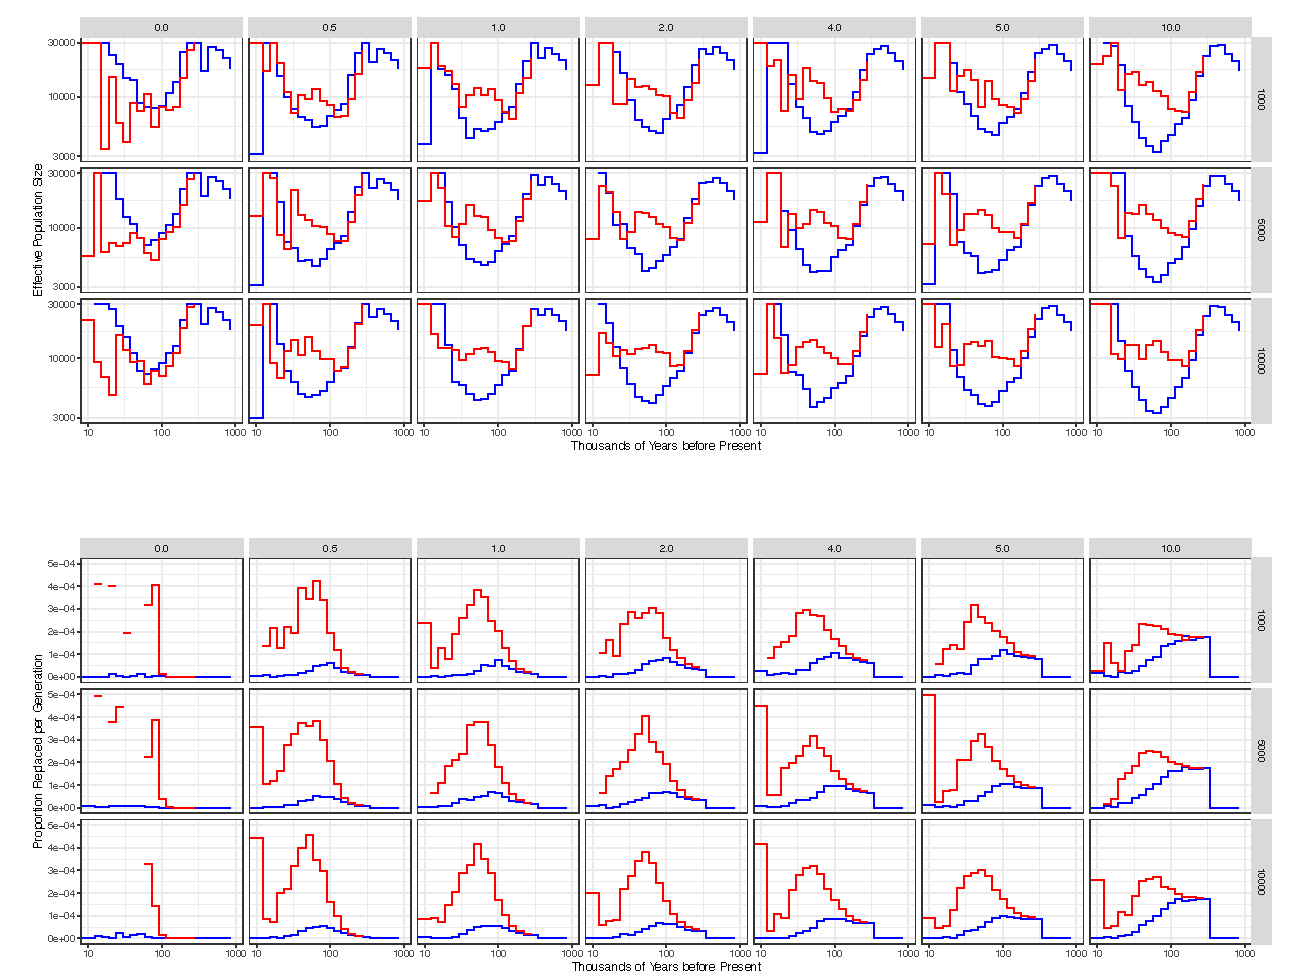
\includegraphics[width=\textwidth]{../plot/mig/yri_dif_migs.pdf}
	\caption{Effective population size and migration history of a Yoruban ({\tt S\_Yoruba-1}) and a French ({\tt S\_French-1}) individual from the Simons Genome Diversity panel. The initial migration proportion was varied along the X axis, while the number of particles is varied along the Y. 10 iterations of variational Bayes was used for parameter inference, while 5000 particles were used to sample from the posterior distribution of trees.}
	\label{init_yri}
\end{figure}

\clearpage
\section{Average $D$ Statistics Among Populations}

Here we consider the case of instantaneous admixture explored by Durand et al 2011 when a representative sample from the admixing population is available. Here, the expectation of $D$ is reduced to 
\small 
$$ \begin{aligned} E[  D(P_2, P_1, P0, O)] 
	&= \frac{\text{Pr(ABBA)} - \text{Pr(BABA)}}{\text{Pr(ABBA)} + \text{Pr(BABA)}} \\
&= \frac{3f[t_{P3} - t_{GF}]}{3f [t_{P3} - t_{GF}] + 4N(1-f) (1 - \frac{1}{2N})^{t_{P3}-  t_{P2}} + 4Nf (1 - \frac{1}{2N})^{t_{P3}-t_{GF}}} \end{aligned}$$

where $t_{P_i}$ is the expected time to coalescence of any two lineages in $P_i$, $f$ is the proportion of gene flow while $t_{GF}$ is its timing, and $N$ is the population size. We consider the case where $D$ statistics $D(A_i, A_{pi}, Y, C)$ are summed and divided by their count. In this case, both $A_i$ and $A_{pi}$ are drawn from the same population, which implies that $t_{P_3}$ is constant (with the exception of the San, who are excluded from these calculations). Since we assume that $t_{P_3}$, $f$, $t_{GF}$ are held constant, we straightforwardly rearrange the definition of the $D$ statistic to show that the expectation of averaging over the log of $D$ values for $n$ populations gives the expectation of a $D$ statistic with the average $t_{P2}$, or time to divergence of lineages within the population.  

\resizebox{.75\linewidth}{!}{
	\begin{minipage}{\linewidth}
	$$ \begin{aligned}
	\mathbb{E} [\frac{1}{n} \sum^n_i \ln D(P2, P1, P0, O)] &= \frac{1}{n} \sum^n_i \mathbb{E}[ \ln D(P2, P1, P0, O)] \\
	&= \frac{1}{n} \sum^n_i \ln \frac{3f[t_{P3} - t_{GF}]}{3f [t_{P3} - t_{GF}] + 4N(1-f) (1 - \frac{1}{2N})^{t_{P3}-  t_{P2}} + 4Nf (1 - \frac{1}{2N})^{t_{P3}-t_{GF}}} \\
	&= \frac{1}{n} \sum^n_i \ln \left( 3f[t_{P3} - t_{GF} \right) - \ln ( 3f [t_{P3} - t_{GF}] + 4N(1-f) (1 - \frac{1}{2N})^{t_{P3}-  t_{P2}} \\  &+ 4Nf (1 - \frac{1}{2N})^{t_{P3}-t_{GF}}) \\
	&= \frac{1}{n} \sum^n_i \ln \left( 3f[t_{P3} - t_{GF} \right) - \ln \left( 3f [t_{P3} - t_{GF}] \right) + \ln \left( 4N(1-f) (1 - \frac{1}{2N})^{t_{P3}-  t_{P2}} \right) \\  &- \ln \left( 4Nf (1 - \frac{1}{2N})^{t_{P3}-t_{GF}} \right) \\
	&= \frac{1}{n} \left( n \left( \ln \left( 3f[t_{P3} - t_{GF} \right) + \ln \left( 3f [t_{P3} - t_{GF}] \right) +  + \ln \left( 4Nf (1 - \frac{1}{2N})^{t_{P3}-t_{GF}} \right) \right) \right) \\ &+ \sum^n_i \ln \left( 4N(1-f) (1 - \frac{1}{2N})^{t_{P3}-  t_{P2}} \right) \\
	&= \ldots \sum^n_i (t_{P3}-  t_{P2} ) \ln \left( 4N(1-f) (1 - \frac{1}{2N}) \right) \\
	&= \ldots n \ln \left( 4N(1-f) (1 - \frac{1}{2N}) \right) \sum^n_i (t_{P3}-  t_{P2} ) \\
	&= \ldots n \ln \left( 4N(1-f) (1 - \frac{1}{2N}) \right) \left( \sum^n_i t_{P3} - \sum^n_i t_{P2} \right) \\
	&= \ldots n t_{P3}\ln \left( 4N(1-f) (1 - \frac{1}{2N}) \right) \left(- \sum^n_i t_{P2} \right) \\
	& \text{multiply through the } \frac{1}{n} \ldots \\
	&= \ln \left( 3f[t_{P3} - t_{GF} \right) + \ln \left( 3f [t_{P3} - t_{GF}] \right) +  \ln \left( 4Nf (1 - \frac{1}{2N})^{t_{P3}-t_{GF}} \right) \\ &+ t_{P3} \ln \left( 4N(1-f) (1 - \frac{1}{2N}) \right) \left(- \frac{1}{n} \sum^n_i t_{P2} \right) \\
	&= \ln \left( 3f[t_{P3} - t_{GF} \right) + \ln \left( 3f [t_{P3} - t_{GF}] \right) +  \ln \left( 4Nf (1 - \frac{1}{2N})^{t_{P3}-t_{GF}} \right) \\ &+ \ln \left( 4N(1-f) (1 - \frac{1}{2N})^{t_{P3} - \frac{1}{n} \sum^n_i t_{P2}} \right) \\
	&= \ln \frac{3f[t_{P3} - t_{GF}]}{3f [t_{P3} - t_{GF}] + 4N(1-f) (1 - \frac{1}{2N})^{t_{P3}-  \frac{1}{n} \sum^n_i t_{P2}} + 4Nf (1 - \frac{1}{2N})^{t_{P3}-t_{GF}}} \\
	&= \ln D(\bar{P2}, \bar{P1}, P0, O)
	\end{aligned} $$
\end{minipage}
}

Therefore, the expectation of average $D$ statistics where both $P_1$ and $P_2$ are drawn from the same population produces the expectation of the $D$ statistic with the average within-population coalescent rate. 

\end{document}
